%&preformat-disser
\RequirePackage[l2tabu,orthodox]{nag} % Раскомментировав, можно в логе получать рекомендации относительно правильного использования пакетов и предупреждения об устаревших и нерекомендуемых пакетах
% Формат А4, 14pt (ГОСТ Р 7.0.11-2011, 5.3.6)
\documentclass[a4paper,14pt,oneside,openany]{memoir}

\input{common/setup}               % общие настройки шаблона
%%% Проверка используемого TeX-движка %%%
\usepackage{iftex}[2013/04/04]
\newif\ifxetexorluatex   % определяем новый условный оператор (http://tex.stackexchange.com/a/47579/79756)
\ifXeTeX
    \xetexorluatextrue
\else
    \ifLuaTeX
        \xetexorluatextrue
    \else
        \xetexorluatexfalse
    \fi
\fi

\RequirePackage{etoolbox}[2015/08/02]               % Для продвинутой проверки разных условий

%%% Поля и разметка страницы %%%
\usepackage{pdflscape}                              % Для включения альбомных страниц
\usepackage{geometry}                               % Для последующего задания полей

%%% Математические пакеты %%%
\usepackage{amsthm,amsfonts,amsmath,amssymb,amscd}  % Математические дополнения от AMS
\usepackage{mathtools}                              % Добавляет окружение multlined

%%%% Установки для размера шрифта 14 pt %%%%
%% Формирование переменных и констант для сравнения (один раз для всех подключаемых файлов)%%
%% должно располагаться до вызова пакета fontspec или polyglossia, потому что они сбивают его работу
\newlength{\curtextsize}
\newlength{\bigtextsize}
\setlength{\bigtextsize}{13.9pt}

\makeatletter
%\show\f@size                                       % неплохо для отслеживания, но вызывает стопорение процесса, если документ компилируется без команды  -interaction=nonstopmode 
\setlength{\curtextsize}{\f@size pt}
\makeatother

%%% Кодировки и шрифты %%%
\ifxetexorluatex
    \usepackage{csquotes}
    \usepackage{polyglossia}[2014/05/21]            % Поддержка многоязычности (fontspec подгружается автоматически)
\else
    \RequirePDFTeX                                  % tests for PDFTEX use and throws an error if a different engine is being used
   %%% Решение проблемы копирования текста в буфер кракозябрами
%    \input glyphtounicode.tex
%    \input glyphtounicode-cmr.tex %from pdfx package
%    \pdfgentounicode=1
    \usepackage{cmap}                               % Улучшенный поиск русских слов в полученном pdf-файле
    \defaulthyphenchar=127                          % Если стоит до fontenc, то переносы не впишутся в выделяемый текст при копировании его в буфер обмена
    \usepackage[T2A]{fontenc}                       % Поддержка русских букв
    \usepackage[utf8]{inputenc}[2014/04/30]         % Кодировка utf8
    \usepackage[english, russian]{babel}[2014/03/24]% Языки: русский, английский
    \IfFileExists{pscyr.sty}{\usepackage{pscyr}}{}  % Красивые русские шрифты
\fi

%%% Оформление абзацев %%%
\usepackage{indentfirst}                            % Красная строка

%%% Цвета %%%
\usepackage[dvipsnames,usenames]{color}
\usepackage{colortbl}
%\usepackage[dvipsnames, table, hyperref, cmyk]{xcolor} % Вероятно, более новый вариант, вместо предыдущих двух строк. Конвертация всех цветов в cmyk заложена как удовлетворение возможного требования типографий. Возможно конвертирование и в rgb.

%%% Таблицы %%%
\usepackage{longtable}                              % Длинные таблицы
\usepackage{multirow,makecell}                      % Улучшенное форматирование таблиц

%%% Общее форматирование
\usepackage{soulutf8}                               % Поддержка переносоустойчивых подчёркиваний и зачёркиваний
\usepackage{icomma}                                 % Запятая в десятичных дробях


%%% Гиперссылки %%%
\usepackage{hyperref}[2012/11/06]

%%% Изображения %%%
\usepackage{graphicx}[2014/04/25]                   % Подключаем пакет работы с графикой

%%% Списки %%%
\usepackage{enumitem}

%%% Подписи %%%
\usepackage{caption}[2013/05/02]                    % Для управления подписями (рисунков и таблиц) % Может управлять номерами рисунков и таблиц с caption %Иногда может управлять заголовками в списках рисунков и таблиц
\usepackage{subcaption}[2013/02/03]                 % Работа с подрисунками и подобным

%%% Счётчики %%%
\usepackage[figure,table]{totalcount}               % Счётчик рисунков и таблиц
\usepackage{totcount}                               % Пакет создания счётчиков на основе последнего номера подсчитываемого элемента (может требовать дважды компилировать документ)
\usepackage{totpages}                               % Счётчик страниц, совместимый с hyperref (ссылается на номер последней страницы). Желательно ставить последним пакетом в преамбуле

%%% Продвинутое управление групповыми ссылками (пока только формулами) %%%
\ifxetexorluatex
    \usepackage{cleveref}                           % cleveref корректно считывает язык из настроек polyglossia
\else
    \usepackage[russian]{cleveref}                  % cleveref имеет сложности со считыванием языка из babel. Такое решение русификации вывода выбрано вместо определения в documentclass из опасности что-то лишнее передать во все остальные пакеты, включая библиографию.
\fi
\creflabelformat{equation}{#2#1#3}                  % Формат по умолчанию ставил круглые скобки вокруг каждого номера ссылки, теперь просто номера ссылок без какого-либо дополнительного оформления


\ifnumequal{\value{draft}}{1}{% Черновик
    \usepackage[firstpage]{draftwatermark}
    \SetWatermarkText{DRAFT}
    \SetWatermarkFontSize{14pt}
    \SetWatermarkScale{15}
    \SetWatermarkAngle{45}
}{}

  % Пакеты общие для диссертации и автореферата
%%% Прикладные пакеты %%% 
%\usepackage{calc}               % Пакет для расчётов параметров, например длины

%%% Для добавления Стр. над номерами страниц в оглавлении
%%% http://tex.stackexchange.com/a/306950
\usepackage{afterpage}
         % Пакеты для диссертации
%%% Микротипографика %%%
%\ifnumequal{\value{draft}}{0}{% Только если у нас режим чистовика
%    \usepackage[final]{microtype}[2016/05/14] % улучшает представление букв и слов в строках, может помочь при наличии отдельно висящих слов
%}{}
\usepackage{amsmath}
\usepackage{tikz}
        % Пакеты для специфических пользовательских задач

\input{Dissertation/setup}               % Упрощённые настройки шаблона

\input{Dissertation/preamblenames}       % Переопределение именований, чтобы можно было и в преамбуле использовать
\input{common/newnames}  % Новые переменные, которые могут использоваться во всём проекте

%%% Основные сведения %%%
\newcommand{\thesisAuthor}             % Диссертация, ФИО автора
{%
    \texorpdfstring{% \texorpdfstring takes two arguments and uses the first for (La)TeX and the second for pdf
        Быков Евгений Михайлович% так будет отображаться на титульном листе или в тексте, где будет использоваться переменная
    }{%
        Быков, Евгений, Михайлович% эта запись для свойств pdf-файла. В таком виде, если pdf будет обработан программами для сбора библиографических сведений, будет правильно представлена фамилия.
    }%
}

\newcommand{\thesisAuthorShort}        % Диссертация, ФИО автора инициалами
{\todo{Е.М.~Быков}}

\newcommand{\thesisUdk}                % Диссертация, УДК
{\todo{xxx.xxx}}
\newcommand{\thesisTitle}              % Диссертация, название
{\texorpdfstring{\MakeUppercase{Анализ и разработка современных интеллектуальных механизмов управления критической инфраструктурой  с применением методов машинного обучения}}{Название диссертационной работы}}
\newcommand{\thesisSpecialtyNumber}    % Диссертация, специальность, номер
{\texorpdfstring{05.13.01 }}
\newcommand{\thesisSpecialtyTitle}     % Диссертация, специальность, название
{\texorpdfstring{Системный анализ, управление и обработка информации (по отраслям)}{Название специальности}}
\newcommand{\thesisDegree}             % Диссертация, ученая степень
{кандидата технических наук}
\newcommand{\thesisDegreeShort}        % Диссертация, ученая степень, краткая запись
{канд. техн. наук}
\newcommand{\thesisCity}               % Диссертация, город защиты
{Москва}
\newcommand{\thesisYear}               % Диссертация, год защиты
{2018}
\newcommand{\thesisOrganization}       % Диссертация, организация
{Московский Физико-Технический Институт}
\newcommand{\thesisOrganizationShort}  % Диссертация, краткое название организации для доклада
{\todo{НазУчДисРаб}}

\newcommand{\thesisInOrganization}     % Диссертация, организация в предложном падеже: Работа выполнена в ...
{\todo{ автономной некоммерческой образовательной организации высшего профессионального образований \enquote{Сколковский институт науки и технологий}}}

\newcommand{\supervisorFio}            % Научный руководитель, ФИО
{Кулешов Александр Петрович}
\newcommand{\supervisorRegalia}        % Научный руководитель, регалии
{доктор технических наук, академик РАН}
\newcommand{\supervisorFioShort}       % Научный руководитель, ФИО
{\todo{А.П.~Кулешов}}
\newcommand{\supervisorRegaliaShort}   % Научный руководитель, регалии
{\todo{д.т.н., академик}}


\newcommand{\opponentOneFio}           % Оппонент 1, ФИО
{\todo{Фамилия Имя Отчество}}
\newcommand{\opponentOneRegalia}       % Оппонент 1, регалии
{\todo{доктор физико-математических наук, профессор}}
\newcommand{\opponentOneJobPlace}      % Оппонент 1, место работы
{\todo{Не очень длинное название для места работы}}
\newcommand{\opponentOneJobPost}       % Оппонент 1, должность
{\todo{старший научный сотрудник}}

\newcommand{\opponentTwoFio}           % Оппонент 2, ФИО
{\todo{Фамилия Имя Отчество}}
\newcommand{\opponentTwoRegalia}       % Оппонент 2, регалии
{\todo{кандидат физико-математических наук}}
\newcommand{\opponentTwoJobPlace}      % Оппонент 2, место работы
{\todo{Основное место работы c длинным длинным длинным длинным названием}}
\newcommand{\opponentTwoJobPost}       % Оппонент 2, должность
{\todo{старший научный сотрудник}}

\newcommand{\leadingOrganizationTitle} % Ведущая организация, дополнительные строки
{\todo{Федеральное государственное бюджетное образовательное учреждение высшего профессионального образования с~длинным длинным длинным длинным названием}}

\newcommand{\defenseDate}              % Защита, дата
{\todo{DD июля 2018 г.~в~XX часов}}
\newcommand{\defenseCouncilNumber}     % Защита, номер диссертационного совета
{\todo{Д\,212.156.0..}}
\newcommand{\defenseCouncilTitle}      % Защита, учреждение диссертационного совета
{\todo{Название учреждения}}
\newcommand{\defenseCouncilAddress}    % Защита, адрес учреждение диссертационного совета
{\todo{Адрес}}
\newcommand{\defenseCouncilPhone}      % Телефон для справок
{\todo{+7~(985)~128-37-08}}

\newcommand{\defenseSecretaryFio}      % Секретарь диссертационного совета, ФИО
{\todo{Фамилия Имя Отчество}}
\newcommand{\defenseSecretaryRegalia}  % Секретарь диссертационного совета, регалии
{\todo{д-р~физ.-мат. наук}}            % Для сокращений есть ГОСТы, например: ГОСТ Р 7.0.12-2011 + http://base.garant.ru/179724/#block_30000

\newcommand{\synopsisLibrary}          % Автореферат, название библиотеки
{\todo{Название библиотеки}}
\newcommand{\synopsisDate}             % Автореферат, дата рассылки
{\todo{DD mmmmmmmm YYYY года}}

% To avoid conflict with beamer class use \providecommand
\providecommand{\keywords}%            % Ключевые слова для метаданных PDF диссертации и автореферата
{}
      % Основные сведения
%%% Кодировки и шрифты %%%
\ifxetexorluatex
    \setmainlanguage[babelshorthands=true]{russian}  % Язык по-умолчанию русский с поддержкой приятных команд пакета babel
    \setotherlanguage{english}                       % Дополнительный язык = английский (в американской вариации по-умолчанию)
    \setmonofont{Courier New}
    \newfontfamily\cyrillicfonttt{Courier New}
    \ifXeTeX
        \defaultfontfeatures{Ligatures=TeX,Mapping=tex-text}
    \else
        \defaultfontfeatures{Ligatures=TeX}
    \fi
    \setmainfont{Times New Roman}
    \newfontfamily\cyrillicfont{Times New Roman}
    \setsansfont{Arial}
    \newfontfamily\cyrillicfontsf{Arial}
\else
    \IfFileExists{pscyr.sty}{\renewcommand{\rmdefault}{ftm}}{}
\fi

%%% Подписи %%%
\captionsetup{%
singlelinecheck=off,                % Многострочные подписи, например у таблиц
skip=2pt,                           % Вертикальная отбивка между подписью и содержимым рисунка или таблицы определяется ключом
justification=centering,            % Центрирование подписей, заданных командой \caption
}

%%% Рисунки %%%
\DeclareCaptionLabelSeparator*{emdash}{~--- }             % (ГОСТ 2.105, 4.3.1)
\captionsetup[figure]{labelsep=emdash,position=bottom}

%%% Таблицы %%%
\ifnumequal{\value{tabcap}}{0}{%
    \newcommand{\tabcapalign}{\raggedright}  % по левому краю страницы или аналога parbox

    \DeclareCaptionFormat{tablecaption}{\tabcapalign #1#2#3}
    \captionsetup[table]{labelsep=emdash}                       % тире как разделитель идентификатора с номером от наименования
}{%
    \ifnumequal{\value{tablaba}}{0}{%
        \newcommand{\tabcapalign}{\raggedright}  % по левому краю страницы или аналога parbox
    }{}

    \ifnumequal{\value{tablaba}}{1}{%
        \newcommand{\tabcapalign}{\centering}    % по центру страницы или аналога parbox
    }{}

    \ifnumequal{\value{tablaba}}{2}{%
        \newcommand{\tabcapalign}{\raggedleft}   % по правому краю страницы или аналога parbox
    }{}

    \ifnumequal{\value{tabtita}}{0}{%
        \newcommand{\tabtitalign}{\raggedright}  % по левому краю страницы или аналога parbox
    }{}

    \ifnumequal{\value{tabtita}}{1}{%
        \newcommand{\tabtitalign}{\centering}    % по центру страницы или аналога parbox
    }{}

    \ifnumequal{\value{tabtita}}{2}{%
        \newcommand{\tabtitalign}{\raggedleft}   % по правому краю страницы или аналога parbox
    }{}

    \DeclareCaptionFormat{tablecaption}{\tabcapalign #1#2\par%  % Идентификатор таблицы на отдельной строке
        \tabtitalign{#3}}                                       % Наименование таблицы строкой ниже
    \captionsetup[table]{labelsep=space}                        % пробельный разделитель идентификатора с номером от наименования
}
\DeclareCaptionFormat{tablenocaption}{\tabcapalign #1\strut}    % Наименование таблицы отсутствует

\captionsetup[table]{format=tablecaption,singlelinecheck=off,position=top,skip=0pt}  % многострочные наименования и прочее
\DeclareCaptionLabelFormat{continued}{Продолжение таблицы~#2}

%%% Подписи подрисунков %%%
\renewcommand{\thesubfigure}{\asbuk{subfigure}}           % Буквенные номера подрисунков
\captionsetup[subfigure]{font={normalsize},               % Шрифт подписи названий подрисунков (не отличается от основного)
    labelformat=brace,                                    % Формат обозначения подрисунка
    justification=centering,                              % Выключка подписей (форматирование), один из вариантов            
}
%\DeclareCaptionFont{font12pt}{\fontsize{12pt}{13pt}\selectfont} % объявляем шрифт 12pt для использования в подписях, тут же надо интерлиньяж объявлять, если не наследуется
%\captionsetup[subfigure]{font={font12pt}}                 % Шрифт подписи названий подрисунков (всегда 12pt)

%%% Настройки гиперссылок %%%
\ifLuaTeX
    \hypersetup{
        unicode,                % Unicode encoded PDF strings
    }
\fi

\hypersetup{
    linktocpage=true,           % ссылки с номера страницы в оглавлении, списке таблиц и списке рисунков
%    linktoc=all,                % both the section and page part are links
%    pdfpagelabels=false,        % set PDF page labels (true|false)
    plainpages=false,           % Forces page anchors to be named by the Arabic form  of the page number, rather than the formatted form
    colorlinks,                 % ссылки отображаются раскрашенным текстом, а не раскрашенным прямоугольником, вокруг текста
    linkcolor={linkcolor},      % цвет ссылок типа ref, eqref и подобных
    citecolor={citecolor},      % цвет ссылок-цитат
    urlcolor={urlcolor},        % цвет гиперссылок
%    hidelinks,                  % Hide links (removing color and border)
    pdftitle={\thesisTitle},    % Заголовок
    pdfauthor={\thesisAuthor},  % Автор
    pdfsubject={\thesisSpecialtyNumber\ \thesisSpecialtyTitle},      % Тема
%    pdfcreator={Создатель},     % Создатель, Приложение
%    pdfproducer={Производитель},% Производитель, Производитель PDF
    pdfkeywords={\keywords},    % Ключевые слова
    pdflang={ru},
}
\ifnumequal{\value{draft}}{1}{% Черновик
    \hypersetup{
        draft,
    }
}{}

%%% Шаблон %%%
\DeclareRobustCommand{\todo}{\textcolor{red}}       % решаем проблему превращения названия цвета в результате \MakeUppercase, http://tex.stackexchange.com/a/187930/79756 , \DeclareRobustCommand protects \todo from expanding inside \MakeUppercase
\AtBeginDocument{%
    \setlength{\parindent}{2.5em}                   % Абзацный отступ. Должен быть одинаковым по всему тексту и равен пяти знакам (ГОСТ Р 7.0.11-2011, 5.3.7).
}

%%% Списки %%%
% Используем короткое тире (endash) для ненумерованных списков (ГОСТ 2.105-95, пункт 4.1.7, требует дефиса, но так лучше смотрится)
\renewcommand{\labelitemi}{\normalfont\bfseries{--}}

% Перечисление строчными буквами латинского алфавита (ГОСТ 2.105-95, 4.1.7)
%\renewcommand{\theenumi}{\alph{enumi}}
%\renewcommand{\labelenumi}{\theenumi)} 

% Перечисление строчными буквами русского алфавита (ГОСТ 2.105-95, 4.1.7)
\makeatletter
\AddEnumerateCounter{\asbuk}{\russian@alph}{щ}      % Управляем списками/перечислениями через пакет enumitem, а он 'не знает' про asbuk, потому 'учим' его
\makeatother
%\renewcommand{\theenumi}{\asbuk{enumi}} %первый уровень нумерации
%\renewcommand{\labelenumi}{\theenumi)} %первый уровень нумерации 
\renewcommand{\theenumii}{\asbuk{enumii}} %второй уровень нумерации
\renewcommand{\labelenumii}{\theenumii)} %второй уровень нумерации 
\renewcommand{\theenumiii}{\arabic{enumiii}} %третий уровень нумерации
\renewcommand{\labelenumiii}{\theenumiii)} %третий уровень нумерации 

\setlist{nosep,%                                    % Единый стиль для всех списков (пакет enumitem), без дополнительных интервалов.
    labelindent=\parindent,leftmargin=*%            % Каждый пункт, подпункт и перечисление записывают с абзацного отступа (ГОСТ 2.105-95, 4.1.8)
}
    % Стили общие для диссертации и автореферата
%%% Изображения %%%
\graphicspath{{images/}{Dissertation/images/}}         % Пути к изображениям

%%% Макет страницы %%%
% Выставляем значения полей (ГОСТ 7.0.11-2011, 5.3.7)
\geometry{a4paper,top=2cm,bottom=2cm,left=2.5cm,right=1cm,nofoot,nomarginpar} %,showframe
\setlength{\topskip}{0pt}   %размер дополнительного верхнего поля

%%% Интервалы %%%
%% По ГОСТ Р 7.0.11-2011, пункту 5.3.6 требуется полуторный интервал
%% Реализация средствами класса (на основе setspace) ближе к типографской классике.
%% И правит сразу и в таблицах (если со звёздочкой) 
%\DoubleSpacing*     % Двойной интервал
\OnehalfSpacing*    % Полуторный интервал
%\setSpacing{1.42}   % Полуторный интервал, подобный Ворду (возможно, стоит включать вместе с предыдущей строкой)

%%% Выравнивание и переносы %%%
%% http://tex.stackexchange.com/questions/241343/what-is-the-meaning-of-fussy-sloppy-emergencystretch-tolerance-hbadness
%% http://www.latex-community.org/forum/viewtopic.php?p=70342#p70342
\tolerance 1414
\hbadness 1414
\emergencystretch 1.5em % В случае проблем регулировать в первую очередь
\hfuzz 0.3pt
\vfuzz \hfuzz
%\raggedbottom
%\sloppy                 % Избавляемся от переполнений
\clubpenalty=10000      % Запрещаем разрыв страницы после первой строки абзаца
\widowpenalty=10000     % Запрещаем разрыв страницы после последней строки абзаца

%%% Блок управления параметрами для выравнивания заголовков в тексте %%%
\newlength{\otstuplen}
\setlength{\otstuplen}{\theotstup\parindent}
\ifnumequal{\value{headingalign}}{0}{% выравнивание заголовков в тексте
    \newcommand{\hdngalign}{\centering}                % по центру
    \newcommand{\hdngaligni}{}% по центру
    \setlength{\otstuplen}{0pt}
}{%
    \newcommand{\hdngalign}{}                 % по левому краю
    \newcommand{\hdngaligni}{\hspace{\otstuplen}}      % по левому краю
} % В обоих случаях вроде бы без переноса, как и надо (ГОСТ Р 7.0.11-2011, 5.3.5)

%%% Оглавление %%%
\renewcommand{\cftchapterdotsep}{\cftdotsep}                % отбивка точками до номера страницы начала главы/раздела

%% Переносить слова в заголовке не допускается (ГОСТ Р 7.0.11-2011, 5.3.5). Заголовки в оглавлении должны точно повторять заголовки в тексте (ГОСТ Р 7.0.11-2011, 5.2.3). Прямого указания на запрет переносов в оглавлении нет, но по той же логике невнесения искажений в смысл, лучше в оглавлении не переносить:
\setrmarg{2.55em plus1fil}                             %To have the (sectional) titles in the ToC, etc., typeset ragged right with no hyphenation
\renewcommand{\cftchapterpagefont}{\normalfont}        % нежирные номера страниц у глав в оглавлении
\renewcommand{\cftchapterleader}{\cftdotfill{\cftchapterdotsep}}% нежирные точки до номеров страниц у глав в оглавлении
%\renewcommand{\cftchapterfont}{}                       % нежирные названия глав в оглавлении

\ifnumgreater{\value{headingdelim}}{0}{%
    \renewcommand\cftchapteraftersnum{.\space}       % добавляет точку с пробелом после номера раздела в оглавлении
}{}
\ifnumgreater{\value{headingdelim}}{1}{%
    \renewcommand\cftsectionaftersnum{.\space}       % добавляет точку с пробелом после номера подраздела в оглавлении
    \renewcommand\cftsubsectionaftersnum{.\space}    % добавляет точку с пробелом после номера подподраздела в оглавлении
    \renewcommand\cftsubsubsectionaftersnum{.\space} % добавляет точку с пробелом после номера подподподраздела в оглавлении
    \AtBeginDocument{% без этого polyglossia сама всё переопределяет
        \setsecnumformat{\csname the#1\endcsname.\space}
    }
}{%
    \AtBeginDocument{% без этого polyglossia сама всё переопределяет
        \setsecnumformat{\csname the#1\endcsname\quad}
    }
}

\renewcommand*{\cftappendixname}{\appendixname\space} % Слово Приложение в оглавлении

%%% Колонтитулы %%%
% Порядковый номер страницы печатают на середине верхнего поля страницы (ГОСТ Р 7.0.11-2011, 5.3.8)
\makeevenhead{plain}{}{\thepage}{}
\makeoddhead{plain}{}{\thepage}{}
\makeevenfoot{plain}{}{}{}
\makeoddfoot{plain}{}{}{}
\pagestyle{plain}

%%% добавить Стр. над номерами страниц в оглавлении
%%% http://tex.stackexchange.com/a/306950
\newif\ifendTOC

\newcommand*{\tocheader}{
\ifnumequal{\value{pgnum}}{1}{%
    \ifendTOC\else\hbox to \linewidth%
      {\noindent{}~\hfill{Стр.}}\par%
      \ifnumless{\value{page}}{3}{}{%
        \vspace{0.5\onelineskip}
      }
      \afterpage{\tocheader}
    \fi%
}{}%
}%

%%% Оформление заголовков глав, разделов, подразделов %%%
%% Работа должна быть выполнена ... размером шрифта 12-14 пунктов (ГОСТ Р 7.0.11-2011, 5.3.8). То есть не должно быть надписей шрифтом более 14. Так и поставим.
%% Эти установки будут давать одинаковый результат независимо от выбора базовым шрифтом 12 пт или 14 пт
\newcommand{\basegostsectionfont}{\fontsize{14pt}{16pt}\selectfont\bfseries}

\makechapterstyle{thesisgost}{%
    \chapterstyle{default}
    \setlength{\beforechapskip}{0pt}
    \setlength{\midchapskip}{0pt}
    \setlength{\afterchapskip}{\theintvl\curtextsize}
    \renewcommand*{\chapnamefont}{\basegostsectionfont}
    \renewcommand*{\chapnumfont}{\basegostsectionfont}
    \renewcommand*{\chaptitlefont}{\basegostsectionfont}
    \renewcommand*{\chapterheadstart}{}
    \ifnumgreater{\value{headingdelim}}{0}{%
        \renewcommand*{\afterchapternum}{.\space}   % добавляет точку с пробелом после номера раздела
    }{%
        \renewcommand*{\afterchapternum}{\quad}     % добавляет \quad после номера раздела
    }
    \renewcommand*{\printchapternum}{\hdngaligni\hdngalign\chapnumfont \thechapter}
    \renewcommand*{\printchaptername}{}
    \renewcommand*{\printchapternonum}{\hdngaligni\hdngalign}
}

\makeatletter
\makechapterstyle{thesisgostchapname}{%
    \chapterstyle{thesisgost}
    \renewcommand*{\printchapternum}{\chapnumfont \thechapter}
    \renewcommand*{\printchaptername}{\hdngaligni\hdngalign\chapnamefont \@chapapp} %
}
\makeatother

\chapterstyle{thesisgost}

\setsecheadstyle{\basegostsectionfont\hdngalign}
\setsecindent{\otstuplen}

\setsubsecheadstyle{\basegostsectionfont\hdngalign}
\setsubsecindent{\otstuplen}

\setsubsubsecheadstyle{\basegostsectionfont\hdngalign}
\setsubsubsecindent{\otstuplen}

\sethangfrom{\noindent #1} %все заголовки подразделов центрируются с учетом номера, как block 

\ifnumequal{\value{chapstyle}}{1}{%
    \chapterstyle{thesisgostchapname}
    \renewcommand*{\cftchaptername}{\chaptername\space} % будет вписано слово Глава перед каждым номером раздела в оглавлении
}{}%

%%% Интервалы между заголовками
\setbeforesecskip{\theintvl\curtextsize}% Заголовки отделяют от текста сверху и снизу тремя интервалами (ГОСТ Р 7.0.11-2011, 5.3.5).
\setaftersecskip{\theintvl\curtextsize}
\setbeforesubsecskip{\theintvl\curtextsize}
\setaftersubsecskip{\theintvl\curtextsize}
\setbeforesubsubsecskip{\theintvl\curtextsize}
\setaftersubsubsecskip{\theintvl\curtextsize}

%%% Блок дополнительного управления размерами заголовков
\ifnumequal{\value{headingsize}}{1}{% Пропорциональные заголовки и базовый шрифт 14 пт
    \renewcommand{\basegostsectionfont}{\large\bfseries}
    \renewcommand*{\chapnamefont}{\Large\bfseries}
    \renewcommand*{\chapnumfont}{\Large\bfseries}
    \renewcommand*{\chaptitlefont}{\Large\bfseries}
}{}

%%% Счётчики %%%

%% Упрощённые настройки шаблона диссертации: нумерация формул, таблиц, рисунков
\ifnumequal{\value{contnumeq}}{1}{%
    \counterwithout{equation}{chapter} % Убираем связанность номера формулы с номером главы/раздела
}{}
\ifnumequal{\value{contnumfig}}{1}{%
    \counterwithout{figure}{chapter}   % Убираем связанность номера рисунка с номером главы/раздела
}{}
\ifnumequal{\value{contnumtab}}{1}{%
    \counterwithout{table}{chapter}    % Убираем связанность номера таблицы с номером главы/раздела
}{}


%%http://www.linux.org.ru/forum/general/6993203#comment-6994589 (используется totcount)
\makeatletter
\def\formbytotal#1#2#3#4#5{%
    \newcount\@c
    \@c\totvalue{#1}\relax
    \newcount\@last
    \newcount\@pnul
    \@last\@c\relax
    \divide\@last 10
    \@pnul\@last\relax
    \divide\@pnul 10
    \multiply\@pnul-10
    \advance\@pnul\@last
    \multiply\@last-10
    \advance\@last\@c
    \total{#1}~#2%
    \ifnum\@pnul=1#5\else%
    \ifcase\@last#5\or#3\or#4\or#4\or#4\else#5\fi
    \fi
}
\makeatother

\AtBeginDocument{
%% регистрируем счётчики в системе totcounter
    \regtotcounter{totalcount@figure}
    \regtotcounter{totalcount@table}       % Если иным способом поставить в преамбуле то ошибка в числе таблиц
    \regtotcounter{TotPages}               % Если иным способом поставить в преамбуле то ошибка в числе страниц
}

%%% Правильная нумерация приложений %%%
%% По ГОСТ 2.105, п. 4.3.8 Приложения обозначают заглавными буквами русского алфавита,
%% начиная с А, за исключением букв Ё, З, Й, О, Ч, Ь, Ы, Ъ.
%% Здесь также переделаны все нумерации русскими буквами.
\ifxetexorluatex
    \makeatletter
    \def\russian@Alph#1{\ifcase#1\or
       А\or Б\or В\or Г\or Д\or Е\or Ж\or
       И\or К\or Л\or М\or Н\or
       П\or Р\or С\or Т\or У\or Ф\or Х\or
       Ц\or Ш\or Щ\or Э\or Ю\or Я\else\xpg@ill@value{#1}{russian@Alph}\fi}
    \def\russian@alph#1{\ifcase#1\or
       а\or б\or в\or г\or д\or е\or ж\or
       и\or к\or л\or м\or н\or
       п\or р\or с\or т\or у\or ф\or х\or
       ц\or ш\or щ\or э\or ю\or я\else\xpg@ill@value{#1}{russian@alph}\fi}
    \makeatother
\else
    \makeatletter
    \if@uni@ode
      \def\russian@Alph#1{\ifcase#1\or
        А\or Б\or В\or Г\or Д\or Е\or Ж\or
        И\or К\or Л\or М\or Н\or
        П\or Р\or С\or Т\or У\or Ф\or Х\or
        Ц\or Ш\or Щ\or Э\or Ю\or Я\else\@ctrerr\fi}
    \else
      \def\russian@Alph#1{\ifcase#1\or
        \CYRA\or\CYRB\or\CYRV\or\CYRG\or\CYRD\or\CYRE\or\CYRZH\or
        \CYRI\or\CYRK\or\CYRL\or\CYRM\or\CYRN\or
        \CYRP\or\CYRR\or\CYRS\or\CYRT\or\CYRU\or\CYRF\or\CYRH\or
        \CYRC\or\CYRSH\or\CYRSHCH\or\CYREREV\or\CYRYU\or
        \CYRYA\else\@ctrerr\fi}
    \fi
    \if@uni@ode
      \def\russian@alph#1{\ifcase#1\or
        а\or б\or в\or г\or д\or е\or ж\or
        и\or к\or л\or м\or н\or
        п\or р\or с\or т\or у\or ф\or х\or
        ц\or ш\or щ\or э\or ю\or я\else\@ctrerr\fi}
    \else
      \def\russian@alph#1{\ifcase#1\or
        \cyra\or\cyrb\or\cyrv\or\cyrg\or\cyrd\or\cyre\or\cyrzh\or
        \cyri\or\cyrk\or\cyrl\or\cyrm\or\cyrn\or
        \cyrp\or\cyrr\or\cyrs\or\cyrt\or\cyru\or\cyrf\or\cyrh\or
        \cyrc\or\cyrsh\or\cyrshch\or\cyrerev\or\cyryu\or
        \cyrya\else\@ctrerr\fi}
    \fi
    \makeatother
\fi           % Стили для диссертации
% для вертикального центрирования ячеек в tabulary
\def\zz{\ifx\[$\else\aftergroup\zzz\fi}
%$ \] % <-- чиним подсветку синтаксиса в некоторых редакторах
\def\zzz{\setbox0\lastbox
\dimen0\dimexpr\extrarowheight + \ht0-\dp0\relax
\setbox0\hbox{\raise-.5\dimen0\box0}%
\ht0=\dimexpr\ht0+\extrarowheight\relax
\dp0=\dimexpr\dp0+\extrarowheight\relax 
\box0
}



\lstdefinelanguage{Renhanced}%
{keywords={abbreviate,abline,abs,acos,acosh,action,add1,add,%
        aggregate,alias,Alias,alist,all,anova,any,aov,aperm,append,apply,%
        approx,approxfun,apropos,Arg,args,array,arrows,as,asin,asinh,%
        atan,atan2,atanh,attach,attr,attributes,autoload,autoloader,ave,%
        axis,backsolve,barplot,basename,besselI,besselJ,besselK,besselY,%
        beta,binomial,body,box,boxplot,break,browser,bug,builtins,bxp,by,%
        c,C,call,Call,case,cat,category,cbind,ceiling,character,char,%
        charmatch,check,chol,chol2inv,choose,chull,class,close,cm,codes,%
        coef,coefficients,co,col,colnames,colors,colours,commandArgs,%
        comment,complete,complex,conflicts,Conj,contents,contour,%
        contrasts,contr,control,helmert,contrib,convolve,cooks,coords,%
        distance,coplot,cor,cos,cosh,count,fields,cov,covratio,wt,CRAN,%
        create,crossprod,cummax,cummin,cumprod,cumsum,curve,cut,cycle,D,%
        data,dataentry,date,dbeta,dbinom,dcauchy,dchisq,de,debug,%
        debugger,Defunct,default,delay,delete,deltat,demo,de,density,%
        deparse,dependencies,Deprecated,deriv,description,detach,%
        dev2bitmap,dev,cur,deviance,off,prev,,dexp,df,dfbetas,dffits,%
        dgamma,dgeom,dget,dhyper,diag,diff,digamma,dim,dimnames,dir,%
        dirname,dlnorm,dlogis,dnbinom,dnchisq,dnorm,do,dotplot,double,%
        download,dpois,dput,drop,drop1,dsignrank,dt,dummy,dump,dunif,%
        duplicated,dweibull,dwilcox,dyn,edit,eff,effects,eigen,else,%
        emacs,end,environment,env,erase,eval,equal,evalq,example,exists,%
        exit,exp,expand,expression,External,extract,extractAIC,factor,%
        fail,family,fft,file,filled,find,fitted,fivenum,fix,floor,for,%
        For,formals,format,formatC,formula,Fortran,forwardsolve,frame,%
        frequency,ftable,ftable2table,function,gamma,Gamma,gammaCody,%
        gaussian,gc,gcinfo,gctorture,get,getenv,geterrmessage,getOption,%
        getwd,gl,glm,globalenv,gnome,GNOME,graphics,gray,grep,grey,grid,%
        gsub,hasTsp,hat,heat,help,hist,home,hsv,httpclient,I,identify,if,%
        ifelse,Im,image,\%in\%,index,influence,measures,inherits,install,%
        installed,integer,interaction,interactive,Internal,intersect,%
        inverse,invisible,IQR,is,jitter,kappa,kronecker,labels,lapply,%
        layout,lbeta,lchoose,lcm,legend,length,levels,lgamma,library,%
        licence,license,lines,list,lm,load,local,locator,log,log10,log1p,%
        log2,logical,loglin,lower,lowess,ls,lsfit,lsf,ls,machine,Machine,%
        mad,mahalanobis,make,link,margin,match,Math,matlines,mat,matplot,%
        matpoints,matrix,max,mean,median,memory,menu,merge,methods,min,%
        missing,Mod,mode,model,response,mosaicplot,mtext,mvfft,na,nan,%
        names,omit,nargs,nchar,ncol,NCOL,new,next,NextMethod,nextn,%
        nlevels,nlm,noquote,NotYetImplemented,NotYetUsed,nrow,NROW,null,%
        numeric,\%o\%,objects,offset,old,on,Ops,optim,optimise,optimize,%
        options,or,order,ordered,outer,package,packages,page,pairlist,%
        pairs,palette,panel,par,parent,parse,paste,path,pbeta,pbinom,%
        pcauchy,pchisq,pentagamma,persp,pexp,pf,pgamma,pgeom,phyper,pico,%
        pictex,piechart,Platform,plnorm,plogis,plot,pmatch,pmax,pmin,%
        pnbinom,pnchisq,pnorm,points,poisson,poly,polygon,polyroot,pos,%
        postscript,power,ppoints,ppois,predict,preplot,pretty,Primitive,%
        print,prmatrix,proc,prod,profile,proj,prompt,prop,provide,%
        psignrank,ps,pt,ptukey,punif,pweibull,pwilcox,q,qbeta,qbinom,%
        qcauchy,qchisq,qexp,qf,qgamma,qgeom,qhyper,qlnorm,qlogis,qnbinom,%
        qnchisq,qnorm,qpois,qqline,qqnorm,qqplot,qr,Q,qty,qy,qsignrank,%
        qt,qtukey,quantile,quasi,quit,qunif,quote,qweibull,qwilcox,%
        rainbow,range,rank,rbeta,rbind,rbinom,rcauchy,rchisq,Re,read,csv,%
        csv2,fwf,readline,socket,real,Recall,rect,reformulate,regexpr,%
        relevel,remove,rep,repeat,replace,replications,report,require,%
        resid,residuals,restart,return,rev,rexp,rf,rgamma,rgb,rgeom,R,%
        rhyper,rle,rlnorm,rlogis,rm,rnbinom,RNGkind,rnorm,round,row,%
        rownames,rowsum,rpois,rsignrank,rstandard,rstudent,rt,rug,runif,%
        rweibull,rwilcox,sample,sapply,save,scale,scan,scan,screen,sd,se,%
        search,searchpaths,segments,seq,sequence,setdiff,setequal,set,%
        setwd,show,sign,signif,sin,single,sinh,sink,solve,sort,source,%
        spline,splinefun,split,sqrt,stars,start,stat,stem,step,stop,%
        storage,strstrheight,stripplot,strsplit,structure,strwidth,sub,%
        subset,substitute,substr,substring,sum,summary,sunflowerplot,svd,%
        sweep,switch,symbol,symbols,symnum,sys,status,system,t,table,%
        tabulate,tan,tanh,tapply,tempfile,terms,terrain,tetragamma,text,%
        time,title,topo,trace,traceback,transform,tri,trigamma,trunc,try,%
        ts,tsp,typeof,unclass,undebug,undoc,union,unique,uniroot,unix,%
        unlink,unlist,unname,untrace,update,upper,url,UseMethod,var,%
        variable,vector,Version,vi,warning,warnings,weighted,weights,%
        which,while,window,write,\%x\%,x11,X11,xedit,xemacs,xinch,xor,%
        xpdrows,xy,xyinch,yinch,zapsmall,zip},%
    otherkeywords={!,!=,~,$,*,\%,\&,\%/\%,\%*\%,\%\%,<-,<<-},%$
    alsoother={._$},%$
    sensitive,%
    morecomment=[l]\#,%
    morestring=[d]",%
    morestring=[d]'% 2001 Robert Denham
}%

%решаем проблему с кириллицей в комментариях (в pdflatex) https://tex.stackexchange.com/a/103712/79756
\lstset{extendedchars=true,literate={Ö}{{\"O}}1
    {Ä}{{\"A}}1
    {Ü}{{\"U}}1
    {ß}{{\ss}}1
    {ü}{{\"u}}1
    {ä}{{\"a}}1
    {ö}{{\"o}}1
    {~}{{\textasciitilde}}1
    {а}{{\selectfont\char224}}1
    {б}{{\selectfont\char225}}1
    {в}{{\selectfont\char226}}1
    {г}{{\selectfont\char227}}1
    {д}{{\selectfont\char228}}1
    {е}{{\selectfont\char229}}1
    {ё}{{\"e}}1
    {ж}{{\selectfont\char230}}1
    {з}{{\selectfont\char231}}1
    {и}{{\selectfont\char232}}1
    {й}{{\selectfont\char233}}1
    {к}{{\selectfont\char234}}1
    {л}{{\selectfont\char235}}1
    {м}{{\selectfont\char236}}1
    {н}{{\selectfont\char237}}1
    {о}{{\selectfont\char238}}1
    {п}{{\selectfont\char239}}1
    {р}{{\selectfont\char240}}1
    {с}{{\selectfont\char241}}1
    {т}{{\selectfont\char242}}1
    {у}{{\selectfont\char243}}1
    {ф}{{\selectfont\char244}}1
    {х}{{\selectfont\char245}}1
    {ц}{{\selectfont\char246}}1
    {ч}{{\selectfont\char247}}1
    {ш}{{\selectfont\char248}}1
    {щ}{{\selectfont\char249}}1
    {ъ}{{\selectfont\char250}}1
    {ы}{{\selectfont\char251}}1
    {ь}{{\selectfont\char252}}1
    {э}{{\selectfont\char253}}1
    {ю}{{\selectfont\char254}}1
    {я}{{\selectfont\char255}}1
    {А}{{\selectfont\char192}}1
    {Б}{{\selectfont\char193}}1
    {В}{{\selectfont\char194}}1
    {Г}{{\selectfont\char195}}1
    {Д}{{\selectfont\char196}}1
    {Е}{{\selectfont\char197}}1
    {Ё}{{\"E}}1
    {Ж}{{\selectfont\char198}}1
    {З}{{\selectfont\char199}}1
    {И}{{\selectfont\char200}}1
    {Й}{{\selectfont\char201}}1
    {К}{{\selectfont\char202}}1
    {Л}{{\selectfont\char203}}1
    {М}{{\selectfont\char204}}1
    {Н}{{\selectfont\char205}}1
    {О}{{\selectfont\char206}}1
    {П}{{\selectfont\char207}}1
    {Р}{{\selectfont\char208}}1
    {С}{{\selectfont\char209}}1
    {Т}{{\selectfont\char210}}1
    {У}{{\selectfont\char211}}1
    {Ф}{{\selectfont\char212}}1
    {Х}{{\selectfont\char213}}1
    {Ц}{{\selectfont\char214}}1
    {Ч}{{\selectfont\char215}}1
    {Ш}{{\selectfont\char216}}1
    {Щ}{{\selectfont\char217}}1
    {Ъ}{{\selectfont\char218}}1
    {Ы}{{\selectfont\char219}}1
    {Ь}{{\selectfont\char220}}1
    {Э}{{\selectfont\char221}}1
    {Ю}{{\selectfont\char222}}1
    {Я}{{\selectfont\char223}}1
    {і}{{\selectfont\char105}}1
    {ї}{{\selectfont\char168}}1
    {є}{{\selectfont\char185}}1
    {ґ}{{\selectfont\char160}}1
    {І}{{\selectfont\char73}}1
    {Ї}{{\selectfont\char136}}1
    {Є}{{\selectfont\char153}}1
    {Ґ}{{\selectfont\char128}}1
}

% Ширина текста минус ширина надписи 999
\newlength{\twless}
\newlength{\lmarg}
\setlength{\lmarg}{\widthof{999}}   % ширина надписи 999
\setlength{\twless}{\textwidth-\lmarg}


\lstset{ %
%    language=R,                     %  Язык указать здесь, если во всех листингах преимущественно один язык, в результате часть настроек может пойти только для этого языка
    numbers=left,                   % where to put the line-numbers
    numberstyle=\fontsize{12pt}{14pt}\selectfont\color{Gray},  % the style that is used for the line-numbers
    firstnumber=2,                  % в этой и следующей строках задаётся поведение нумерации 5, 10, 15...
    stepnumber=5,                   % the step between two line-numbers. If it's 1, each line will be numbered
    numbersep=5pt,                  % how far the line-numbers are from the code
    backgroundcolor=\color{white},  % choose the background color. You must add \usepackage{color}
    showspaces=false,               % show spaces adding particular underscores
    showstringspaces=false,         % underline spaces within strings
    showtabs=false,                 % show tabs within strings adding particular underscores
    frame=leftline,                 % adds a frame of different types around the code
    rulecolor=\color{black},        % if not set, the frame-color may be changed on line-breaks within not-black text (e.g. commens (green here))
    tabsize=2,                      % sets default tabsize to 2 spaces
    captionpos=t,                   % sets the caption-position to top
    breaklines=true,                % sets automatic line breaking
    breakatwhitespace=false,        % sets if automatic breaks should only happen at whitespace
%    title=\lstname,                 % show the filename of files included with \lstinputlisting;
    % also try caption instead of title
    basicstyle=\fontsize{12pt}{14pt}\selectfont\ttfamily,% the size of the fonts that are used for the code
%    keywordstyle=\color{blue},      % keyword style
    commentstyle=\color{ForestGreen}\emph,% comment style
    stringstyle=\color{Mahogany},   % string literal style
    escapeinside={\%*}{*)},         % if you want to add a comment within your code
    morekeywords={*,...},           % if you want to add more keywords to the set
    inputencoding=utf8,             % кодировка кода
    xleftmargin={\lmarg},           % Чтобы весь код и полоска с номерами строк была смещена влево, так чтобы цифры не вылезали за пределы текста слева
} 

%http://tex.stackexchange.com/questions/26872/smaller-frame-with-listings
% Окружение, чтобы листинг был компактнее обведен рамкой, если она задается, а не на всю ширину текста
\makeatletter
\newenvironment{SmallListing}[1][]
{\lstset{#1}\VerbatimEnvironment\begin{VerbatimOut}{VerbEnv.tmp}}
{\end{VerbatimOut}\settowidth\@tempdima{%
        \lstinputlisting{VerbEnv.tmp}}
    \minipage{\@tempdima}\lstinputlisting{VerbEnv.tmp}\endminipage}    
\makeatother


\DefineVerbatimEnvironment% с шрифтом 12 пт
{Verb}{Verbatim}
{fontsize=\fontsize{12pt}{14pt}\selectfont}

\newfloat[chapter]{ListingEnv}{lol}{Листинг}

\captionsetup[ListingEnv]{
    format=tablecaption,
    labelsep=space,                 % Точка после номера листинга задается значением period
    singlelinecheck=off,
    position=top
}

\captionsetup[lstlisting]{
    format=tablecaption,
    labelsep=space,                 % Точка после номера листинга задается значением period
    singlelinecheck=off,
    position=top
}

\renewcommand{\lstlistingname}{Листинг}

%Общие счётчики окружений листингов
%http://tex.stackexchange.com/questions/145546/how-to-make-figure-and-listing-share-their-counter
% Если смешивать плавающие и не плавающие окружения, то могут быть проблемы с нумерацией
\makeatletter
\AtBeginDocument{%
    \let\c@ListingEnv\c@lstlisting
    \let\theListingEnv\thelstlisting
    \let\ftype@lstlisting\ftype@ListingEnv % give the floats the same precedence
}
\makeatother

% значок С++ — используйте команду \cpp
\newcommand{\cpp}{%
    C\nolinebreak\hspace{-.05em}%
    \raisebox{.2ex}{+}\nolinebreak\hspace{-.10em}%
    \raisebox{.2ex}{+}%
}

%%%  Чересстрочное форматирование таблиц
%% http://tex.stackexchange.com/questions/278362/apply-italic-formatting-to-every-other-row
\newcounter{rowcnt}
\newcommand\altshape{\ifnumodd{\value{rowcnt}}{\color{red}}{\vspace*{-1ex}\itshape}}
% \AtBeginEnvironment{tabular}{\setcounter{rowcnt}{1}}
% \AtEndEnvironment{tabular}{\setcounter{rowcnt}{0}}


%%% Русская традиция начертания математических знаков
%\renewcommand{\le}{\ensuremath{\leqslant}}
%\renewcommand{\leq}{\ensuremath{\leqslant}}
%\renewcommand{\ge}{\ensuremath{\geqslant}}
%\renewcommand{\geq}{\ensuremath{\geqslant}}
%\renewcommand{\emptyset}{\varnothing}

%%% Русская традиция начертания греческих букв (греческие буквы вертикальные, через пакет upgreek)
%\renewcommand{\epsilon}{\ensuremath{\upvarepsilon}}   %  русская традиция записи
%\renewcommand{\phi}{\ensuremath{\upvarphi}}
%%\renewcommand{\kappa}{\ensuremath{\varkappa}}
%\renewcommand{\alpha}{\upalpha}
%\renewcommand{\beta}{\upbeta}
%\renewcommand{\gamma}{\upgamma}
%\renewcommand{\delta}{\updelta}
%\renewcommand{\varepsilon}{\upvarepsilon}
%\renewcommand{\zeta}{\upzeta}
%\renewcommand{\eta}{\upeta}
%\renewcommand{\theta}{\uptheta}
%\renewcommand{\vartheta}{\upvartheta}
%\renewcommand{\iota}{\upiota}
%\renewcommand{\kappa}{\upkappa}
%\renewcommand{\lambda}{\uplambda}
%\renewcommand{\mu}{\upmu}
%\renewcommand{\nu}{\upnu}
%\renewcommand{\xi}{\upxi}
%\renewcommand{\pi}{\uppi}
%\renewcommand{\varpi}{\upvarpi}
%\renewcommand{\rho}{\uprho}
%%\renewcommand{\varrho}{\upvarrho}
%\renewcommand{\sigma}{\upsigma}
%%\renewcommand{\varsigma}{\upvarsigma}
%\renewcommand{\tau}{\uptau}
%\renewcommand{\upsilon}{\upupsilon}
%\renewcommand{\varphi}{\upvarphi}
%\renewcommand{\chi}{\upchi}
%\renewcommand{\psi}{\uppsi}
%\renewcommand{\omega}{\upomega}
          % Стили для специфических пользовательских задач
\input{biblio/bibliopreamble}% Настройки библиографии из внешнего файла (там же выбор: встроенная или на основе biblatex)

\input{Dissertation/inclusioncontrol}    % Управление компиляцией отдельных частей диссертации

\begin{document}

\input{common/renames}                   % Переопределение именований

% Структура диссертации (ГОСТ Р 7.0.11-2011, 4)
\thispagestyle{empty}

\vspace{0pt plus1fill} %число перед fill = кратность относительно некоторого расстояния fill, кусками которого заполнены пустые места
\begin{flushright}
  \large{На правах рукописи}
  
\includegraphics[height=1.5cm]{personal-signature} 
\end{flushright}

\vspace{0pt plus3fill} %число перед fill = кратность относительно некоторого расстояния fill, кусками которого заполнены пустые места
\begin{center}
\textbf {\large \thesisAuthor}
\end{center}

\vspace{0pt plus3fill} %число перед fill = кратность относительно некоторого расстояния fill, кусками которого заполнены пустые места
\begin{center}
\textbf {\Large \thesisTitle}

\vspace{0pt plus3fill} %число перед fill = кратность относительно некоторого расстояния fill, кусками которого заполнены пустые места
{\large Специальность \thesisSpecialtyNumber\ "---\par <<\thesisSpecialtyTitle>>}

\vspace{0pt plus1.5fill} %число перед fill = кратность относительно некоторого расстояния fill, кусками которого заполнены пустые места
\Large{Автореферат}\par
\large{диссертации на соискание учёной степени\par \thesisDegree}
\end{center}

\vspace{0pt plus4fill} %число перед fill = кратность относительно некоторого расстояния fill, кусками которого заполнены пустые места
\begin{center}
{\large{\thesisCity\ "--- \thesisYear}}
\end{center}

\newpage
% оборотная сторона обложки
\thispagestyle{empty}
\noindent Работа выполнена в \thesisInOrganization

\par\bigskip
\noindent%
\begin{tabularx}{\textwidth}{@{}lX@{}}
    Научный руководитель:   & \supervisorRegalia\par
                              \textbf{\supervisorFio}
    \vspace{0.013\paperheight}\\
    Официальные оппоненты:  &
        \textbf{\opponentOneFio,}\par
        \opponentOneRegalia,\par
        \opponentOneJobPlace,\par
        \opponentOneJobPost\par
            \vspace{0.01\paperheight}
        \textbf{\opponentTwoFio,}\par
        \opponentTwoRegalia,\par
        \opponentTwoJobPlace,\par
        \opponentTwoJobPost
    \vspace{0.013\paperheight} \\
    Ведущая организация:    & \leadingOrganizationTitle
\end{tabularx}
\par\bigskip

\noindent Защита состоится \defenseDate~на~заседании диссертационного совета \defenseCouncilNumber~при \defenseCouncilTitle~по адресу: \defenseCouncilAddress.

\vspace{0.017\paperheight}
\noindent С диссертацией можно ознакомиться в библиотеке \synopsisLibrary.

\vspace{0.017\paperheight}
\noindent Отзывы на автореферат в двух экземплярах, заверенные печатью учреждения, просьба направлять по адресу: \defenseCouncilAddress, ученому секретарю диссертационного совета~\defenseCouncilNumber.

\vspace{0.017\paperheight}
\noindent{Автореферат разослан \synopsisDate.}

\noindent Телефон для справок: \defenseCouncilPhone.

\vspace{0.017\paperheight}
\par\bigskip
\noindent%
\begin{tabularx}{\textwidth}{@{}%
>{\raggedright\arraybackslash}b{18em}
>{\centering\arraybackslash}X
r
@{}}
    Ученый секретарь\par
    диссертационного совета\par
    \defenseCouncilNumber,\par
    \defenseSecretaryRegalia
    &
    
\includegraphics[width=2cm]{secretary-signature}
    &
    \defenseSecretaryFio
\end{tabularx}
           % Титульный лист
% Оглавление (ГОСТ Р 7.0.11-2011, 5.2)
\ifdefmacro{\microtypesetup}{\microtypesetup{protrusion=false}}{} % не рекомендуется применять пакет микротипографики к автоматически генерируемому оглавлению
\tableofcontents*
\addtocontents{toc}{\protect\tocheader}
\endTOCtrue
\ifdefmacro{\microtypesetup}{\microtypesetup{protrusion=true}}{}        % Оглавление
\include{Dissertation/introduction}    % Введение
\chapter{Применение методов машинного обучения к задачам управления инфраструктурой} \label{chapt1}

\section{Обзор задач и подходов в России} \label{sect1_1}

% Мы можем сделать \textbf{жирный текст} и \textit{курсив}.

%\newpage
%============================================================================================================================

% \section{\todo{Обзор литературы}} \label{sect1_2}
% Сошлёмся на библиографию. Одна ссылка: \cite[с.~54]{Sokolov}\cite[с.~36]{Gaidaenko}. Две ссылки: \cite{Sokolov,Gaidaenko}. Много ссылок:  \cite[с.~54]{Lermontov,Management,Borozda} \cite{Lermontov,Management,Borozda,Marketing,Constitution,FamilyCode,Gost.7.0.53,Razumovski,Lagkueva,Pokrovski,Sirotko,Lukina,Methodology,Encyclopedia,Nasirova,Berestova,Kriger}. И ещё немного ссылок: \cite{Article,Book,Booklet,Conference,Inbook,Incollection,Manual,Mastersthesis,Misc,Phdthesis,Proceedings,Techreport,Unpublished}. \cite{medvedev2006jelektronnye, CEAT:CEAT581, doi:10.1080/01932691.2010.513279,Gosele1999161,Li2007StressAnalysis, Shoji199895,test:eisner-sample,AB_patent_Pomerantz_1968,iofis_patent1960}

%Попытка реализовать несколько ссылок на конкретные страницы для стандартной реализации:[\citenum{Sokolov}, с.~54; \citenum{Gaidaenko}, с.~36].

%Несколько источников мультицитата \cites[vii--x, 5, 7]{Sokolov}[v--x, 25, 526]{Gaidaenko} поехали дальше

Ссылки на собственные работы:~\cite{vakbib1, confbib1}

% Сошлёмся на приложения: Приложение \ref{AppendixA}, Приложение \ref{AppendixB2}.

% Сошлёмся на формулу: формула \eqref{eq:equation1}.

% Сошлёмся на изображение: рисунок \ref{img:knuth}.

\subsection{\todo{Где вообще используется ML для решения практических задач}}
Теория обучения машин (machine learning, машинное обучение) находится на стыке прикладной статистики, численных методов оптимизации, дискретного анализа, и за последние 50 лет оформилась в самостоятельную математическую дисциплину. Методы машинного обучения составляют основу ещё более молодой дисциплины — интеллектуального анализа данных (data mining).  \cite{воронцов2009машинное} \cite{marsland2015machine} \cite{conway2012machine}
\todo{Перевести введения из источников}
Использование машинного обучения в медицине \todo{(написать)}: \cite{shipp2002diffuse} \cite{ye2003predicting}

\subsection{\todo{ML в телекоме, Q-learning, reinforcement learning}}

\cite{лаптев2011применение} \cite{Magnusson:2012:SCW:2351316.2351327} \cite{hung2006applying} \cite{nelson2008exploiting} \cite{arisholm2007data} \cite{nguyen2012timely} 
Reinforcement learning is the learning of a mapping from situations to actions so as to maximize a scalar reward or reinforcement signal. The learner is not told which action to take, as in most forms of machine learning, but instead must discover which actions yield the highest reward by trying them. In the most interesting and challenging cases, actions may affect not only the immediate's reward, but also the next situation, and through that all subsequent rewards. These two characteristics-trial-and-error search and delayed reward-are the two most important distinguishing features of reinforcement learning. \cite{book:963927} \cite{sutton1998introduction}



\subsection{\todo{ML, ранжирование, решающие леса, xgboost, boosting}}
Tree boosting is a highly effective and widely used machine learning method. A scalable end-to-end tree boosting system called XGBoost is used widely by data scientists to achieve state-of-the-art results on many machine learning challenges. \cite{DBLP:journals/corr/ChenG16} 

Логические модели широко используются для решения задач распознавания и прогнозирования. Это объясняется хорошей интерпретируемостью моделей, имеющих вид логических закономерностей, высокой прогнозирующей способностью, возможностью обрабатывать разнотипные переменные, выделять наиболее важные факторы. Логическую модель можно строить после группировки объектов некоторым алгоритмом, то есть решать задачу распознавания образов в классе логических решающих функций, где под образами понимаются номера кластеров, приписанные объектам. Существуют и алгоритмы, в которых группировка осуществляется непосредственно в ходе построения логической модели. \cite{бериков2008современные}

\todo{Написать своими словами введение}Machine learning: An artificial intelligence approach\cite{michalski2013machine}

Recently there has been a lot of interest in “ensemble learning” — methods that generate many classifiers and aggregate their results. Two well-known methods are boosting (see, e.g., Shapire et al., 1998) and bagging Breiman (1996) of classification trees. In boosting, successive trees give extra weight to points incorrectly predicted by earlier predictors. In the end, a weighted vote is taken for prediction. In bagging, successive trees do not depend on earlier trees — each is independently constructed using a bootstrap sample of the data set. In the end, a simple majority vote is taken for prediction. Breiman (2001) proposed random forests, which add an additional layer of randomness to bagging. In addition to constructing each tree using a different bootstrap sample of the data, random forests change how the classification or regression trees are constructed. In standard trees, each node is split using the best split among all variables. In a random forest, each node is split using the best among a subset of predictors randomly chosen at that node. This somewhat counterintuitive strategy turns out to perform very well compared to many other classifiers, including discriminant analysis, support vector machines and neural networks, and is robust against overfitting (Breiman, 2001). In addition, it is very user-friendly in the sense that it has only two parameters (the number of variables in the random subset at each node and the number of trees in the forest), and is usually not very sensitive to their values. \cite{liaw2002classification}

%\newpage
%============================================================================================================================

\subsection{Системы диагностирования технических устройств}
\cite{prishepa}

\subsection{Обзор литературы} \label{sect1_2_1}
Попытаюсь скопировать информацию о литературе и сослаться на нее. 

There has recently been some interest in applying machine learning techniques to support the acquisition and adaptation of workflow models. The different learning algorithms, that have been proposed, share some restrictions, which may prevent them from being used in practice. Approaches applying techniques from grammatical inference are restricted to sequential workflows. Other algorithms allowing concurrency require unique activity nodes. This contribution shows how the basic principle of our previous approach to sequential workflow induction can be generalized, so that it is able to deal with concurrency. It does not require unique activity nodes. The presented approach uses a log-likelihood guided search in the space of workflow models, that starts with a most general workflow model containing unique activity nodes. Two split operators are available for specialization. \cite{Herbst2000}



%\newpage
%============================================================================================================================



           % Глава 1
\DeclareRobustCommand{\nomenclature}[2]{%
}

\DeclareRobustCommand{\cyrins}[1]{%
 #1
}

\chapter{Применение машинного обучения к ранжированию инцидентов на Московской железной дороге} \label{chapt2}

\section{Введение}
Московская железная дорога (МЖД) \nomenclature{МЖД}{Московская железная дорога} является крупной железнодорожной сетью, включающей в себя 8.8 тыс. км путей и 549 станций. МЖД оснащена несколькими десятками тысяч устройств автоматической регистрации отказов и предотказных состояний оборудования, сигналы которых обрабатываются операторами Центра управления содержанием инфраструктуры. Поток сигналов о возможных инцидентах очень интенсивен и создает большую нагрузку на операторов Центра, причем около 97\% сигналов оказываются ложными тревогами, связанными с недостатками диагностики и техническим обслуживанием оборудования. С целью оптимизации работы Центра нами была разработана основанная на машинном обучении система предварительного автоматического ранжирования инцидентов. Система представляет собой предсказательную модель, оценивающую вероятность наличия реального предотказного состояния по имеющимся признакам сигнала (типа, места, времени,  продолжительности, повторяемости и др.). Предсказательная модель имеет вид ансамбля решающих деревьев, построенного с помощью алгоритма XGBoost по базе данных из 5 миллионов инцидентов. Предсказательная модель внедрена в ПО Центра и используется в повседневной работе операторов~\cite{bulletin-rzd},~\cite{itivs-2017},~\cite{icmla-2017}.

\section{Cтруктура системы диагностирования и мониторинга устройств ЖАТ}
\subsection{Схема работы Центра управления содержанием инфраструктуры}
Московская железная дорога (МЖД) \nomenclature{МЖД}{Московская железная дорога} является крупной железнодорожной сетью, включающей в себя 8.8 тыс. км путей и 549 станций. МЖД оснащена несколькими десятками тысяч устройств ЖАТ (железнодорожная автоматика и телемеханика), производящих автоматическую регистрацию инцидентов -- отказов и предотказных состояний оборудования. Центр управления содержанием инфраструктуры \nomenclature{ЦУСИ}{Центр управления содержанием инфраструктуры} Московской железной дороги (ЦУСИ МЖД) осуществляет непрерывный мониторинг инцидентов на всех участках железной дороги. 
\nomenclature{ЖАТ}{Железнодорожная автоматика и телемеханика}

Инцидент представляет собой совокупность ситуаций, несущих признаки предотказного состояния (например, кратковременное превышение максимально допустимого напряжения оборудования). Наиболее распространенные типы ситуаций, приводящие к предотказам, показаны на рис \ref{fig:histblue}; всего выделяют около 600 различных типов ситуаций. %(уменьшенное время перекрытия стрелки, понижение сопротивления изоляции, пониженное напряжение на путевом реле и т.п.).  

\begin{figure*}
\centering
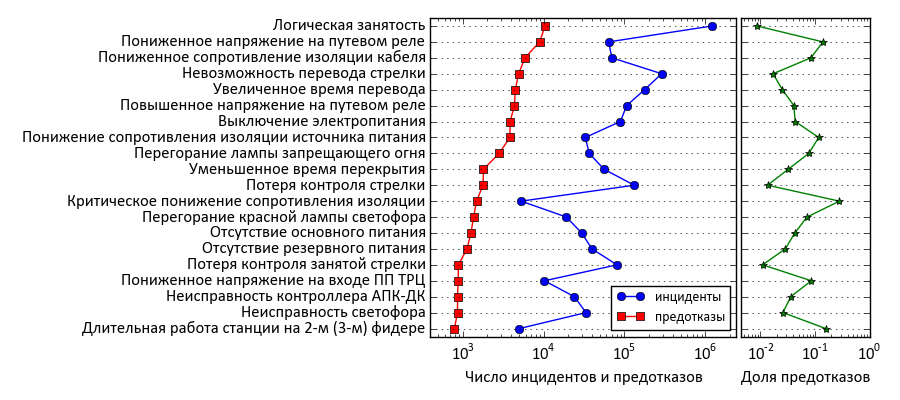
\includegraphics[width=16cm]{incidentsvsfaults-lines.png}
% 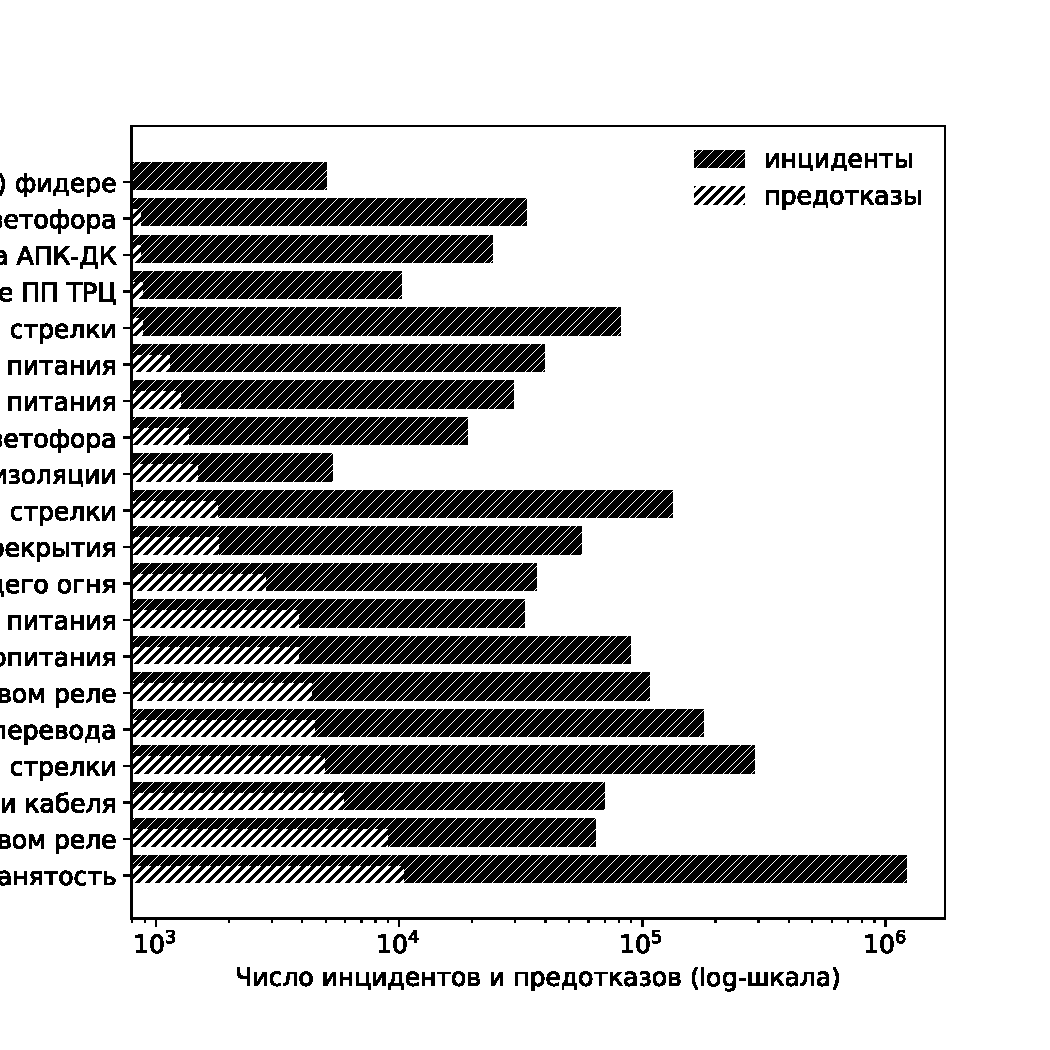
\includegraphics[width=14cm]{incidentsvsfaults-2}
\caption{Наиболее распространённые типы ситуаций, приводящих к предотказу}
\centering
\label{fig:histblue}
\end{figure*}

\begin{figure*}[t]
\centering
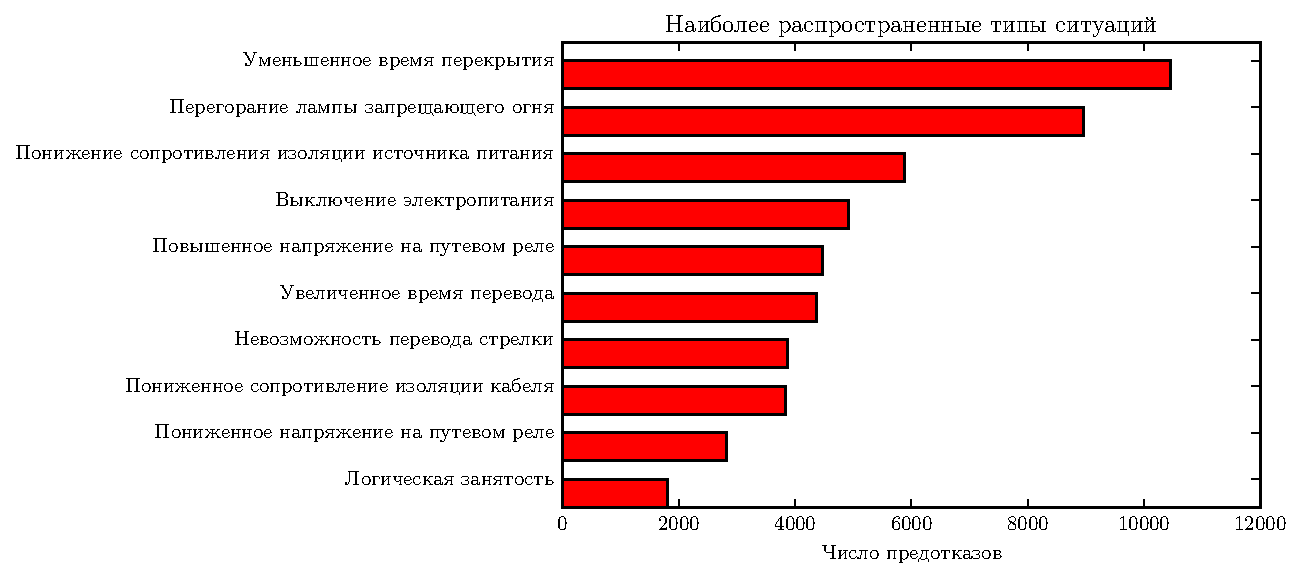
\includegraphics[width=16cm]{redhist}
\caption{Наиболее распространённые типы ситуаций устройств телемеханики, приводящие к предотказу}
\centering
\label{fig:histred}
\end{figure*}

\begin{figure}[t]
\centering
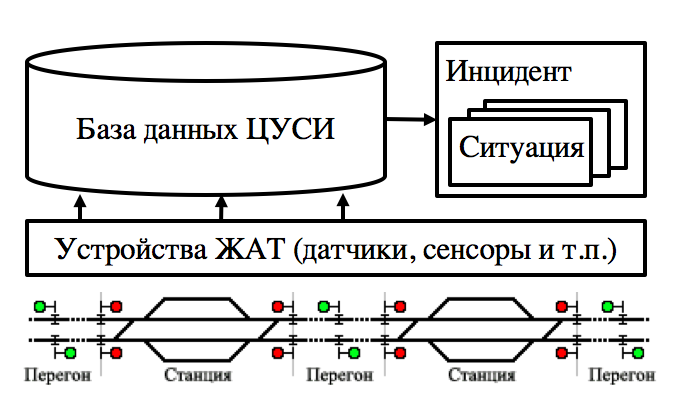
\includegraphics[width=12cm]{arch}
\caption{Последовательность формирования инцидентов: архитектура системы мониторинга}
\centering
\label{fig:arch}
\end{figure}

Ситуации автоматически объединяются в инциденты в базе данных ЦУСИ (см. рис \ref{fig:arch}). Текущие инциденты обрабатываются операторами ЦУСИ, которые выявляют их причины, классифицируют как относящиеся к одному из нескольких типов и принимают необходимые меры. 

Выделяют следующие типы инцидентов (по причине возникновения): предотказное состояние, техническое обслуживание и ремонт, недостатки диагностики и технологическая ситуация. Предотказные состояния образуют наиболее важный тип инцидентов, требующий оперативного реагирования, однако его доля среди всех инцидентов сравнительно невелика (2-3\%). При этом, благодаря достигнутой в последние годы высокой степени обеспечения систем МЖД средствами сбора данных, приходящий в ЦУСИ для обработки операторами поток инцидентов является крайне интенсивным: как правило, новые инциденты могут появляться с интервалом в несколько секунд; общее число инцидентов за 2015 год составило около 1.3 миллионов. 
Таким образом, с точки зрения снижения нагрузки на операторов и повышения эффективности их работы крайне актуальной является задача предварительного автоматического ранжирования инцидентов по степени их важности. В настоящей заметке мы описываем решение этой задачи, полученное нами с помощью методов машинного обучения и внедренное в систему принятия решений ЦУСИ МЖД. 

\subsection{Постановка задачи}
\textbf{Задача} состоит в том, чтобы автоматически классифицировать инциденты, регистрируемые устройствами железнодорожной автоматики и телемеханики,  по их признакам на неисправности, ТОиР и т.п. В качестве \textbf{входных данных} могут использоваться все известные на текущий момент параметры инцидента (признаки места, времени, типа события, показания датчиков и т.п.) и его контекст (например, погода, прошлые инциденты и т.п.). \textbf{Выходные данные}: вероятность того, что инцидент связан с предотказом контролируемого объекта (число от 0 до 1).

\subsection{Описание комплекса АПК-ДК}
Программный комплекс АПК-ДК (Аппаратно-программный комплекс диспетчерского контроля, см. \cite{apk-dk-volkov}, \cite{apk-dk-piter}) разработан ООО «Компьютерные информационные технологии» и научно-исследовательской лабораторией ПГУПС (Петербургский государственный университет путей сообщения).  Система предназначена для контроля и диагностики технического состояния устройств ЖАТ (устройства железнодорожной автоматики и телемеханики).  Комплекс позволяет автоматизировать процессы технического обслуживания устройств и устранения выявленных отказов, а также используется для организации управления движением поездов.

АПК-ДК представляет собой \cite{prishepa}:
\begin{itemize}
	\item аппаратный комплекс контроля и диагностики перегонных и станционных объектов ЖАТ, расположенный на линейных пунктах, включающий в себя АРМ-ШНС (рабочее место старшего электромеханика);
	\item технологический комплекс контроля, диагностики и устранения отказов, расположенный в ШЧ и Ш (включая АРМ-ШЧД, рабочее место диспетчера дистанции);
	\item технологический комплекс центра управления перевозками (включая АРМ-ДНЦ, рабочее место поездного yчастковый диспетчеpа);
	\item подсистема обмена информацией с АОС-ШЧ и АСУ-Ш (включая передачу данных телеконтроля пользователям ПЧ, ЭЧ, ТЧ и другим).
\end{itemize}
АПК-ДК обеспечивает \cite{apk-dk-nesterov}:
\begin{itemize}
	\item просмотр поездного положения:
	\subitem контроль поездного положения и текущего состояния устройств;
	\subitem мониторинг отказов и предотказных состояний;
	\subitem анализ состояния и положения поездных составов за некоторый промежуток времени (до года);
	\subitem контроль движения поездов на основе модели движения с выявлением логических отказов.
	\item просмотр отказов:
	\subitem контроль выявленных ситуаций: с отказами, предотказными состояниями, технологическими ситуациями, проведением ТО, диагностика АПК-ДК;
	\subitem анализ выявленных нарушений (фильтры и группировки);
	\subitem автоматизированная фиксация нарушений в АСУ-Ш.
	\item просмотр параметров:
	\subitem контроль параметров устройств: напряжений, токов, сопротивлений и временных значений;
	\subitem анализ параметров по количественным и качественным критериям на временных графиках за последний год;
	\subitem выявление критичных параметров и сигнализация о них;
	\subitem прогноз времени выхода параметров за норму и другие статистические показатели.
\end{itemize}

Применение в дистанции СЦБ систем АПК-ДК в сопряжении с АСУ-Ш-2 (см. \cite{asu-sh-2}) позволяет автоматизировать учет отказов устройств СЦБ и корректировать план техобслуживания по фактическому состоянию устройств в режиме рельного времени.

\section{Постановка задачи и методика решения}
\subsection{Статистический характер задачи}\label{sec:stat}
Отметим, что важность инцидента можно считать определяемой двумя факторами: вероятностью того, что данный инцидент является реальным предотказным состоянием, и последствиями (в частности, экономическим эффектом) данного отказа. Эти два фактора имеют совершенно разный характер и в значительной степени независимы друг от друга. В то время как вероятность предотказного состояния является предметом статистического анализа на основе лишь сохраненных оперативных данных об инцидентах, оценка последствий отказа предполагает привлечение дополнительных стоимостных моделей отказов и других соображений. В настоящей работе мы акцентируем внимание лишь на первом, вероятностном факторе важности; второй фактор учитывается ЦУСИ МЖД отдельно, с помощью нескольких альтернативных моделей.  
С учетом сделанного замечания цель данной работы можно сформулировать как построение прогнозной модели, которая предсказывает вероятность предотказного состояния для данного инцидента на основе автоматически сформированных данных об этом инциденте.


\subsection{Исходные данные}
Каждый \cyrins{\textit{инцидент}} в базе данных ЦУСИ представляет собой набор \cyrins{\textit{ситуаций}} -- единичных событий, несущих признаки предотказного состояния (например, повышение напряжения, понижение сопротивления и т.п.), см. рис. \ref{fig:arch}. Ситуации автоматически объединяются в инциденты на этапе предварительной обработки сигналов датчиков. В простейшем случае инцидент содержит несколько последовательных однотипных ситуаций (например, несколько случаев кратковременного повышения напряжения на одном и том же приборе), но может содержать и разнотипные ситуации, затрагивающие разное оборудование (например, увеличенное время перевода стрелки и некорректные параметры тока перевода). Количество ситуаций в инциденте может варьироваться от одного до нескольких сотен и может увеличиваться со временем, пока инцидент не рассмотрен и не закрыт оператором ЦУСИ. В общей сложности база данных ЦУСИ содержит около 5 млн. инцидентов, включающих 100 млн. ситуаций.  

Описание каждой ситуации содержит ее тип, время начала и окончания, 
ID места (станции или перегона), ID объекта измерения (прибора) и некоторые другие, менее существенные элементы. Большинство свойств (кроме времени) являются категориальными, причем количество их значений может быть достаточно большим: данные охватывают несколько сот типов ситуаций и мест и около 65000 приборов.

При закрытии инцидента оператором ставится пометка о выявленном типе инцидента, в частности являлся ли он предотказом. 

Таким образом, исторические данные содержат достаточно богатую и хорошо структурированную информацию для построения сложных прогностических моделей вероятности предотказа.    

\subsection{Линейная модель, простое решающее правило}\label{sec:ref_model} 

В качестве примера простой предсказательной модели можно привести прогноз вероятности предотказного состояния исключительно на основе типа первой ситуации инцидента, а именно как долю предотказных инцидентов среди всех наблюдавшихся ранее инцидентов с первой ситуацией данного типа. Это доля сильно зависит от типа ситуации, например, из рис. \ref{fig:histblue} видно, что для ситуации «Критическое понижение сопротивления изоляции» она значительно выше, чем для «Потери контроля занятой стрелки». Поскольку различных типов ситуаций несколько сотен и операторы, очевидно, не в состоянии помнить характеристики каждой из них, даже эта простейшая автоматическая модель ранжирования оказывается практически полезной. В дальнейшем мы будем называть эту модель ``референсной''.  

\subsection{Машинное обучение}
Машинное обучение (МО) \nomenclature{МО}{Машинное обучение} на основе имеющихся исторических данных об инцидентах позволяет строить гораздо более точные предсказательные модели. Стандартная практика машинного обучения \cite{hastie01statisticallearning, Mitchell:1997:ML:541177, scikit-learn} предполагает построение модели в два этапа:
\begin{enumerate}
\item извлечение признаков и формирование обучающей матрицы;
\item применение к полученной обучающей матрице некоторого общего МО-алгоритма.
\end{enumerate}
В ходе первого этапа информация о каждом инциденте приводится к унифицированному виду числового вектора фиксированной размерности, компоненты которого (признаки) отражают потенциально существенные для прогноза характеристики инцидента. Мы описываем этот этап в разделе \ref{sec:feature_extraction}.

В ходе второго этапа к полученной обучающей матрице обычно применяется один из стандартных МО-алгоритмов: логистическая регрессия, нейронные сети, ансамбли решающих деревьев и т.п. Нами использовался алгоритм XGBoost построения ансамбля решающих деревьев с помощью градиентного бустинга \cite{chen2016xgboost}. Мы описываем этот этап в разделе \ref{sec:xgboost}.  

\subsection{Извлечение признаков}\label{sec:feature_extraction}
Извлечение признаков являлось наиболее творческой и трудоемкой частью решения задачи. Оно было связано со следующими трудностями:
\begin{itemize}
\item В общем случае, признаки необходимо агрегировать из всех ситуаций данного инцидента, учитывая, что ситуаций может быть произвольное число. Нами были рассмотрены различные стратегии агрегации, например: ограничиться первой или последней ситуацией в инциденте; в случае числовых признаков взять максимум, минимум или среднее значение по всем ситуациям; в случае категориальных признаков отметить все категории, встреченные в ситуациях инцидентах или сосчитать количество различных встреченных категорий. Конечно, некоторые признаки естественным образом связаны с инцидентом в целом (например, полная продолжительность или место инцидента).
\item Естественным способом преобразования категориального признака с $N$ возможными значениями в числовую форму является его кодирование в виде вектора длины $N$ с единственным ненулевым элементом (one-hot-encoding). Ввиду того, что в рассматриваемой задаче $N$ достигает нескольких сотен или даже тысяч,  обучающие матрицы реализовывались нами в виде разреженных матриц.    
\end{itemize}
С учетом этих обстоятельств, мы рассмотрели несколько десятков различных признаков, описывающих пространственно-временные и прочие характеристики инцидентов. 

Важную роль при создании и отборе признаков играла оценка их значимости, которая осуществлялась нами с помощью двух методов. 
\begin{itemize}
\item
Во-первых, мы оценивали важность признака по общему числу соответствующих ветвлений в итоговой предсказательной модели -- лесе решающих деревьев. Для ``сильно ветвящихся'' признаков мы производили попытку самостоятельно разбить признак на несколько вспомогательных. 
\item Во-вторых, мы реализовали жадный переборный алгоритм последовательного добавления в модель новых признаков, дающих наибольших прирост точности. Этот способ требует многократного обучения модели на различных наборах признаков и поэтому сравнительно долог, однако он позволяет понять, несут ли новые признаки какую-то существенную новую информацию по отношению к уже имеющимся, и какой минимальный набор признаков обеспечивает приемлемую точность модели. Мы подробно описываем результаты этого исследования в разделе \ref{sec:greedy}.
\end{itemize}
Отметим, что помимо признаков, извлекаемых из базы инцидентов, нами была сделана попытка сформировать дополнительные признаки на основе метеоданных, поскольку погодные условия, очевидно, должны оказывать сильное влияние на возникновение некоторых предотказных состояний. Мы действительно обнаружили наличие корреляций между погодными признаками и количеством инцидентов, однако добавление этих признаков в нашу модель не дало заметного улучшения. Иными словами, информация о погоде позволяет улучшить прогноз возникновения инцидента при отсутствии иной информации, но не позволяет заметно улучшить прогноз предотказа при наличии уже имеющейся в базе данных информации об инциденте.


Отметим следующие наблюдения:
\begin{itemize}
\item Как обсуждается далее в разделе \ref{sec:efficiency}, включение в обучающую выборку признаков, родственных уже имеющимся, не дает прироста точности прогноза.
При этом оказалось довольно эффективным сформировать несколько различных признаков, зависящих лишь от времени (полная продолжительность инцидента, время суток и день недели, максимальная продолжительность ситуаций и др.).
\item Погодные условия, очевидно, должны оказывать сильное влияние на возникновение некоторых инцидентов. Нами была сделана попытка привлечь метеоданные для улучшения точности предсказательной модели, однако добавление соответствующих признаков не привело к заметному улучшению. С другой стороны, мы действительно наблюдали наличие корреляций между погодными признаками и количеством инцидентов. Иными словами, информация о погоде позволяет улучшить прогноз возникновения инцидента при отсутствии иной информации, но не позволяет заметно улучшить прогноз предотказа при наличии уже имеющейся в базе данных информации об инциденте.  
\end{itemize}

\subsection{Ансамбль решающих деревьев}\label{sec:xgboost}
Предсказательная модель строилась нами с помощью библиотеки XGboost \cite{chen2016xgboost}. Эта открытая библиотека, хорошо зарекомендовавшая себя в большом числе задач анализа данных\cite{chen2016xgboost}. За последнее время XGBoost неоднократно использовался для решения индустриальных задач, таких как предсказание потребления топлива \cite{horituchi2017predicting}, сбоев технологических процессов (\cite{bosch,DBLP:conf/bigdataconf/Hebert16}), и различных свойств химических составов(\cite{sheridan2016extreme,babajide2016bioactive}). XGboost содержит эффективную реализацию градиентного бустинга \cite{friedman2001greedy}, поддерживающую большие выборки и разреженные матрицы, что было важно в данном проекте. Предсказательная модель представляется в виде суммы ансамбля  бинарных решающих деревьев, последовательно добавляемых в ходе обучения. 

Заметим, что референсная модель из раздела  \ref{sec:ref_model} также естественным образом реализуется в виде ансамбля решающих деревьев, построенных по одному категориальному признаку -- типу первого инцидента. А именно, она состоит из тривиальных деревьев глубины 1 (``решающих пней''), по одному на каждую из компонент бинарного вектора, кодирующего этот категориальный признак. Таким образом, наша основная модель является естественным обобщением референсной модели на случай произвольного набора признаков, числа деревьев и их глубины.

Основная модель была обучена по 3 годам исторических данных (около 5.3 млн. инцидентов) и включала в себя 4000 деревьев глубины 10. Подбор параметров модели осуществлялся стандартным образом с помощью тестирования на контрольной части обучающей выборки.

\subsection{Признаки инцидентов}\label{sec:feature_extraction}
Как уже упоминалось, каждый инцидент представляется как набор ситуаций; каждая ситуация характеризуется своим типом, временем и местом проявления, прибором, на котором она наблюдалась, и некоторыми другими сведениями. Ниже приведены основные признаки инцидентов, получаемые на вход при ранжировании. Перед применением алгоритмов машинного обучения, на основании указанных признаков, порождается расширенный набор признаков, описывающие более сложные свойства. 
Например, 

Признаки типа и количества ситуаций:
\begin{enumerate}
\item Типы всех ситуаций в инциденте
\item Типы всех отказавших объектов
\item Тип первой ситуации 
\item Тип первого отказавшего объекта
\item Общее количество ситуаций
\item Количество различных объектов
\item Количество различных типов ситуаций
\end{enumerate}

Признаки времени:
\begin{enumerate}
\item Время наступления каждой ситуации инцидента
\item Время завершения: аналогично
\item Продолжительность инцидента
\item Время между первой и второй ситуацией
\item Время последнего обновления
\end{enumerate}

Признаки места:

\begin{enumerate}
\item Принадлежность инцидента станции или перегону
\item Принадлежность дистанции
\end{enumerate}
Прочие признаки:

\begin{enumerate}
\item «Тревожность» инцидента (экспертная эвристическая оценка)
\end{enumerate}


\subsection{Предлагаемый подход на основе машинного обучения}
Современные методы машинного обучения позволяют, добиться гораздо большей точности прогноза путем учета большого числа признаков предотказного состояния в рамках сложной логической структуры, массива всех исторических наблюдений. В рамках предложенного подхода была предложена следующая стратегия порождения решающего правила.

\subsubsection{Подготовка исходных данных}
Ниже описывается процедура предварительной обработки исходных данных, содержащихся в базе инцидентов.
\begin{itemize}
\item Исправление пропусков и некорректных значений. На этом этапе для каждого признака порождается дополнительный признак – индикатор некорректного значения. Для численных признаков значение заменяется средним значением, для категориальных – индикатором пропуска.
\item Нормализация распределений численных переменных. На этом этапе подбирается трансформация, преобразующая множество значений величины в отрезок [0;1]. 
\item Текстовые и категориальные признаки бинаризуются, категориальный признак с множеством значений размера N заменяется разреженной матрицей с N+1 столбцами. На практике встречающиеся редко величины признаков принято объединять в один признак. В данной работе такой подход не использовался. Вместо этого производился анализ значимости каждого признака с последующим выбором наиболее важных.
\end{itemize}

Параметры соответствующих преобразований над множеством признаков сохраняются индивидуально для каждого признака. Эти преобразования далее применяются повторно при обработке инцидентов в реальном времени.

\subsubsection{Порождение сложных признаков}
Самый трудоемкий этап подготовки массива данных – порождение сложных признаков из множества простых, хранящихся в базе данных. При порождении такого рода признаков требуется следить за тем, что аналогичные признаки могли бы быть посчитаны не только по историческому массиву данных, но и в оперативном режиме работы классификатора. 

\begin{itemize}
\item Из исходного признака времени порождаются признаки выходных и праздничных дней, времени суток. В качестве независимых признаков выделяются также номера дня в году, месяце и неделе, номер месяца, час, минута и секунда начала инцидента.
\item Признаки времени и места также дополнялись признаками погодных условий – давление, температура, влажность и скорость ветра.
\item Признаки территориальной принадлежности (номер дистанции, номер объекта) дополняются кластеризующими признаками. В нашем случае для кластеризации удалось воспользоваться номером объекта в базе данных (объекты в базе нумеруются последовательно с внедрением и неявно несут информацию о времени и месте установки).
\item Признаки, характеризующие частоту поступления инцидентов для того или иного типа объекта ЖАТ (стрелки, светофоры, рельсовые цепи) для разных временных промежутков (от 1 минуты до месяца). Аналогичные составные признаки были выделены для различных мест обнаружения инцидентов (станция, перегон и т.д.).
\end{itemize}

\subsubsection{Исследование важности порожденных признаков}
Заключительный этап подготовки данных заключается в проверке статистической значимости переменных в модели. Этот шаг выполняется, чтобы отбросить шумящие переменные. Для оценки значимости признаков в данной работе использовалось два подхода.

Первый подход заключается в исследовании поведения показателя AUC при добавлении нового признака на вход обучаемого классификатора. В этом случае для ускорения расчетов мы используем заниженное значение количества раундов обучения и жадный алгоритм выбора очередного признака. Более важным признаком будем считать такой признак, при добавлении которого достигается максимальное увеличение площади под операционной характеристикой классификатора. Эффективность каждого отдельного признака показана на \ref{fig:initialFeatureScores}. На рисунке \ref{fig:adaptiveAdditionScores} можно увидеть последовательное изменение величины показателя AUC при добавлении новых признаков. На рисунке \ref{fig:featureHeatmap} показано насколько больший прирост дает добавляемый признак по сравнению с еще не добавленными.

Второй подход заключается в изучении количественных характеристик итогового решающего правила (леса решающих деревьев) на всем множестве признаков после прохода раундов обучения. В этом случае более важным признаком будем считать такой признак, которому соответствует большее суммарное количество разветвлений в итоговом решающем правиле. Для "сильно ветвящийся" признаков мы производили попытку самостоятельно разбить признак на несколько вспомогательных.

\begin{figure*}
\centering
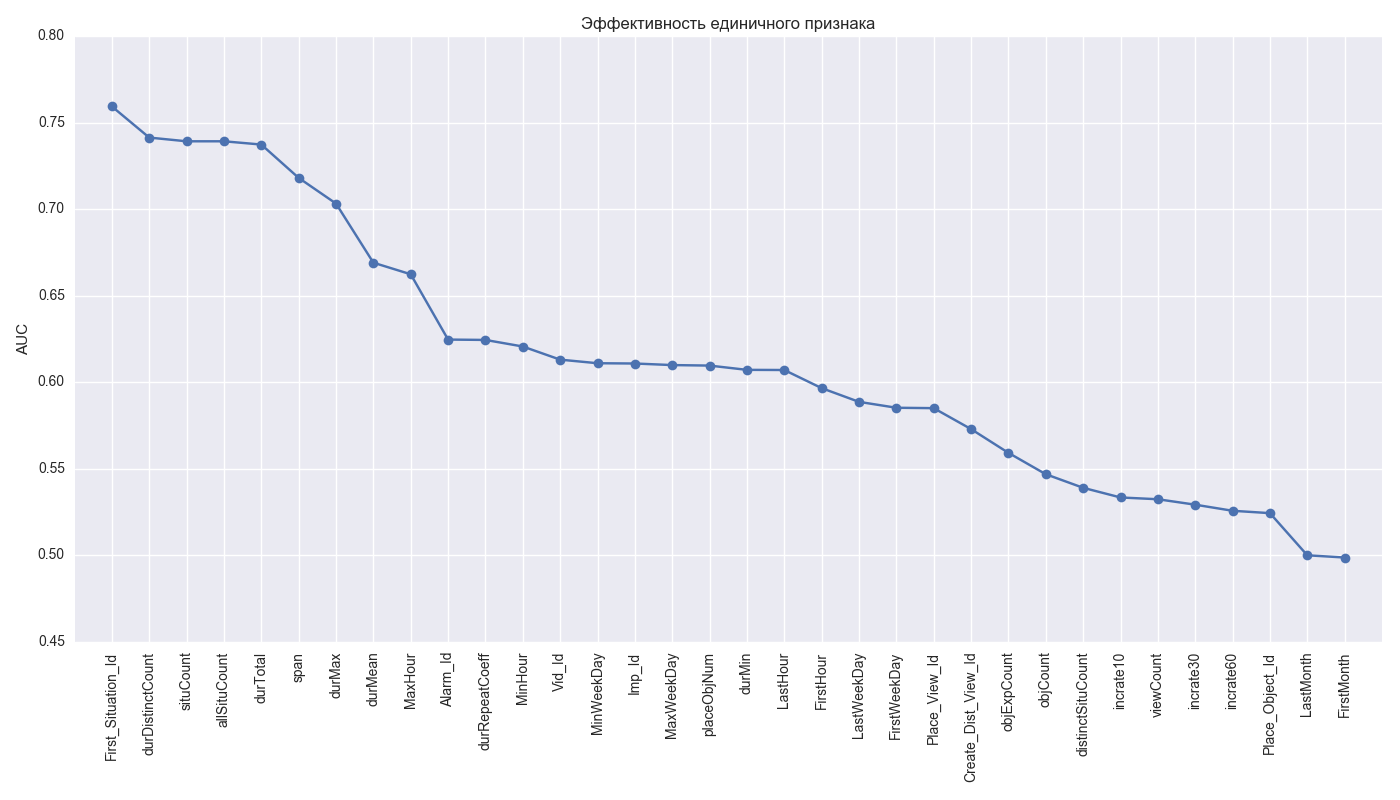
\includegraphics[width=16cm]{initialFeatureScores}
\caption{Анализ важности признаков: эффективность отдельных признаков}
\centering
\label{fig:initialFeatureScores}
\end{figure*}



\begin{figure*}
\centering
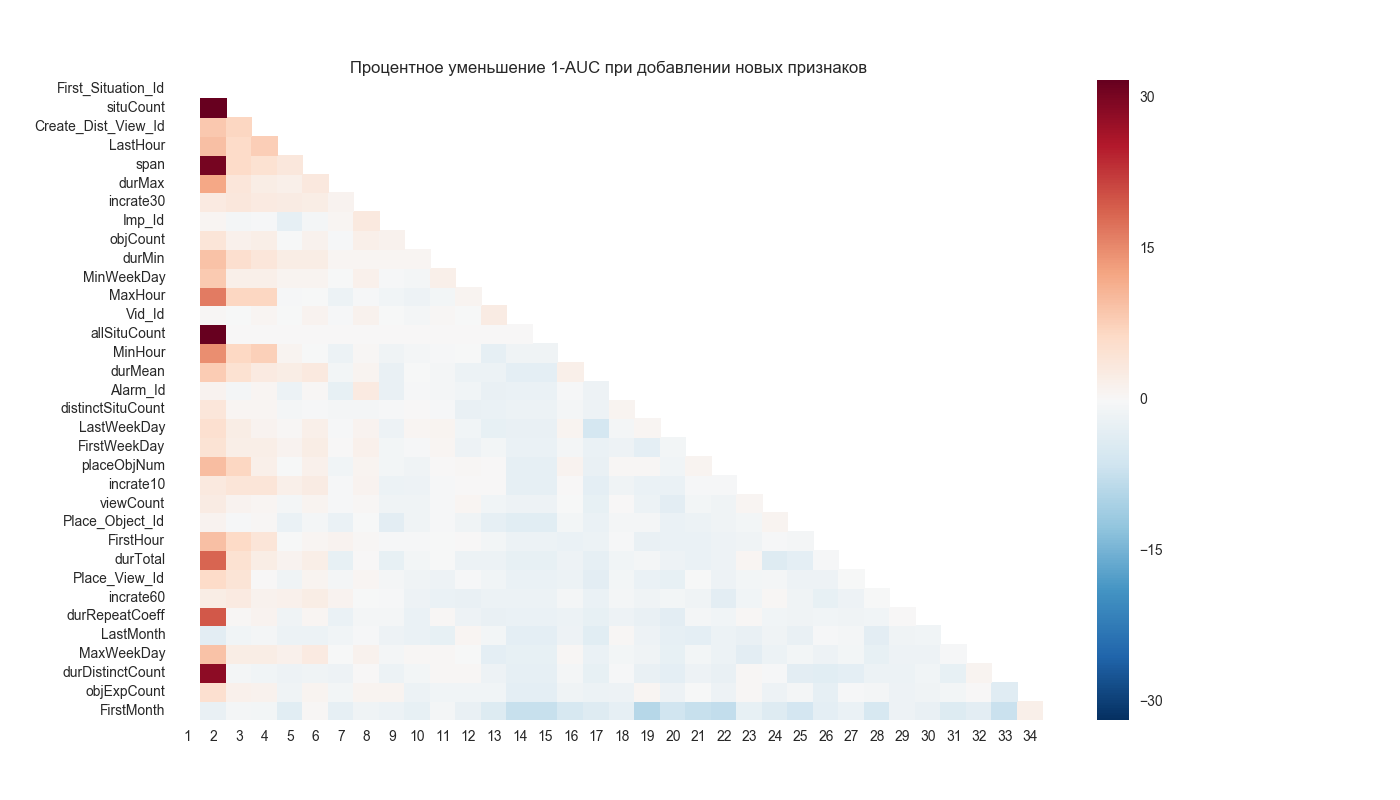
\includegraphics[width=16cm]{featureHeatmap}
\caption{Анализ важности признаков: последовательное добавление}
\centering
\label{fig:featureHeatmap}
\end{figure*}

\subsubsection{Настройка параметров обучения}
Перед настройкой параметров алгоритма исходная выборка инцидентов разделяется на обучающую и контрольную подвыборки. Выбор параметров обучения производится по следующей стратегии.
На начальном этапе при помощи скользящего контроля по тестовой выборке выбирается количество решающих деревьев (\textit{n\_estimators}). Между оптимальными значениями скорости обучения (eta) и количеством решающих деревьев (\textit{n\_estimators}) существует естественная зависимость – чем ниже скорость обучения, тем больше деревьев необходимо, чтобы достичь максимальной точности. После выбора достаточно высокой скорости обучения (0.1 – 0.2) мы итеративно увеличиваем количество деревьев, пока падает ошибка кросс-валидации и переходим к следующему этапу. На следующем этапе подстраиваются параметры решающих деревьев, ответственные за контроль переобучения: \textit{max\_depth}, \textit{min\_child weight}, \textit{gamma}. На последнем этапе производим обучение классификатора с меньшей скоростью обучения (0.025 – 0.1).

\subsubsection{Характеристики решающего правила}
Построенная нами высокоточная прогнозная модель имеет вид ансамбля глубоких решающих деревьев \cite{friedman2001greedy} 
включает в себя 4000 деревьев глубины 10. Пример одного дерева показан на рис. \ref{fig:tree}.

\begin{figure}
\centering
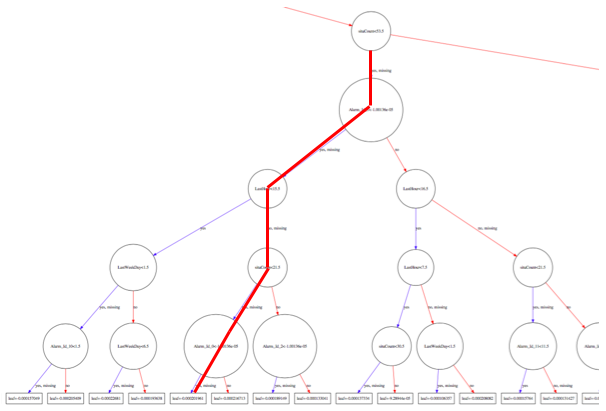
\includegraphics[width=0.7\textwidth]{gr_path}
\caption{Пример прохода по решающему дереву: Если в инциденте: а) количество ситуаций меньше 53, б) последняя ситуация произошла позже 15:30
и в) тревожность равна 1, то повысить вероятность предотказа.
}
\centering
\label{fig:tree}
\end{figure}

Пример цепочки решающих правил, отвечающих проходу по одной ветви дерева, показан на рис. 5. Окончательный прогноз вероятности предотказа получается усреднением прогнозов по всем деревьям.

\section{Анализ модели}

%\pagecolor{yellow!30!orange}
\begin{figure}[thpb] 
\centering
% \includegraphics[width=7cm]{histo2}
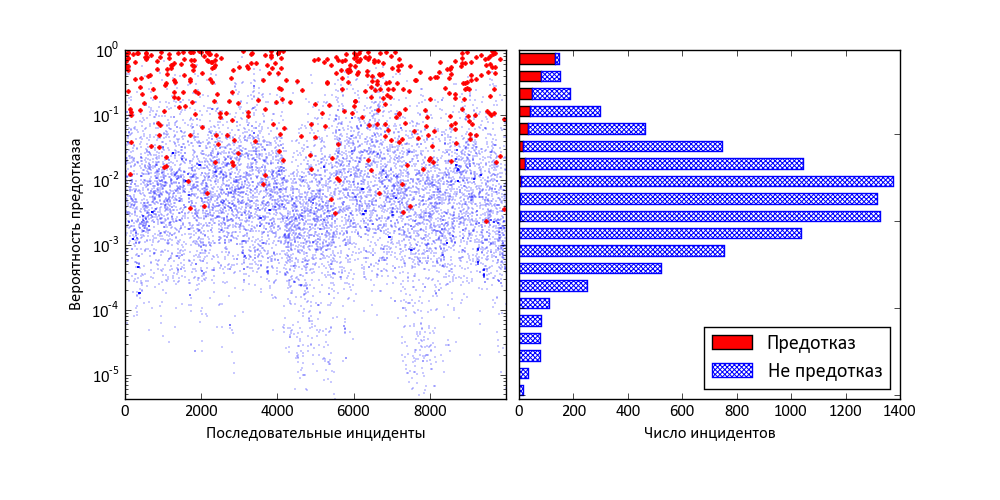
\includegraphics[trim=7mm 7mm 11mm 5mm, clip, width=\textwidth]{threswall-plus.png}
\caption{Результаты ранжирования 10000 последовательных инцидентов.  Предотказы показаны крупными точками, ложные тревоги -- мелкими. В правой части рисунка показаны соответствующие гистограммы распределения инцидентов по вероятности.}
\centering
\label{fig:histo}
\end{figure}


\subsection{Тестовое ранжирование}

В соответствии со стандартной практикой машинного обучения, тестирование построенной модели проводилось на тестовой выборке, изолированной от обучающей выборки, причем обучающие инциденты предшествовали по времени тестовым. 

На рисунке \ref{fig:histo} приведены результаты ранжирования 10000 последовательных инцидентов. Крупные точки показывают инциденты, связанные с предотказами, а мелкие -- инциденты, связанные с ложными срабатываниями системы. Хорошо видно, что основная масса предотказов имеет высокую вероятность и визуально отделена по вероятности от основной массы ложных тревог, имеющей меньшую вероятность. Это свидетельствует о пригодности использования предсказательной модели в качестве ранжирующей функции.

Из рисунка очевидна некоторая неравномерность и периодичность распределения вероятности предотказа в зависимости от номера инцидента. Этот эффект объясняется суточным циклом (показанные 10000 инцидентов отвечают временному интервалу продолжительностью около 3 дней). В дневное время значительное число инцидентов связано с техническим обслуживанием и ремонтом; модель присваивает низкую вероятность предотказа таким инцидентам.


Следует отметить, что существенная доля предотказов имеет после классификации значение вероятности в промежутке 0.001 и 0.1. Для удобства восприятия, это значение выводится на экран инженера службы мониторинга в логарифмической шкале. На рисунке 6 представлена гистограмма распределения значения ранга после логарифмического преобразования. Видно, что большинство инцидентов, связанных с предотказами, находится в промежутке 0.5 – 1.0. 

\subsection{Количественные оценки эффективности ранжирования}
Для количественной оценки эффективности ранжирования мы используем кривую ошибок, определяемую следующим образом. Предположим, что операторы успевают обрабатывать лишь некоторую долю всех инцидентов; рассмотрим соответствующую переменную ДОИ (Доля Обработанных Инцидентов) со значениями в интервале $[0,1]$. Будем считать, что операторы в первую очередь обрабатывают те инциденты, для которых модель предсказывает наиболее высокую вероятность отказа. Пусть величина ДОО (Доля Охваченных Отказов), также со значениями в интервале $[0,1]$, обозначает долю обрабатываемых при этом предотказных инцидентов среди всех предотказных инцидентов. Кривая ошибок тогда представляет собой график зависимости ДОО от ДОИ.

\nomenclature{AUC}{Area Under Curve (англ.), площадь под кривой ошибок}
\nomenclature{ДОИ}{Доля обработанных инцидентов}
\nomenclature{ДОО}{Доля охваченных отказов} 

\begin{figure}[thb] 
\centering
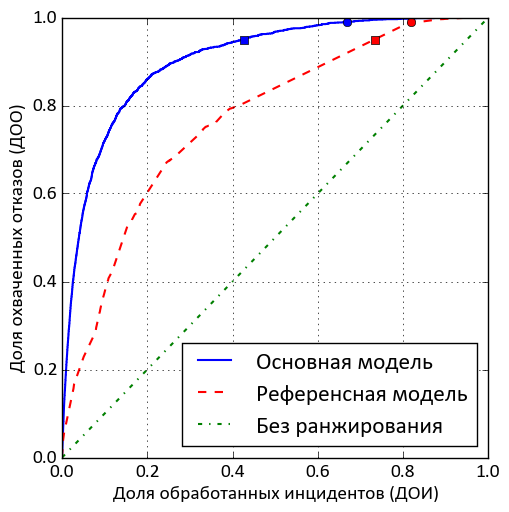
\includegraphics[width=0.5\textwidth]{latexRoc.png}
\caption{Кривые ошибок и связанные с ними характеристики для основной и референсной моделей. Выделенные точки отвечают ДОО 0.95 и  0.99.}\label{fig:ROCcurves} 
\end{figure}

\begin{table} [htbp]
  \label{tbl:aucresults}
  \centering
  %\captionsetup{width=15cm}
  \caption{Количественные результаты ранжирования}\label{Ts0Sib}%
\begin{tabular}{ l c c c}
\toprule
\cyrins{\textbf{Модель}} & \cyrins{\textbf{AUC}} & \cyrins{\textbf{ДОИ95\%}} & \cyrins{\textbf{ДОИ99\%}} \\ \midrule
Основная & 0.904& 0.427 & 0.669 \\
Референсная & 0.768 & 0.733 & 0.818\\
\bottomrule
\end{tabular}
\end{table}

На рис. \ref{fig:ROCcurves} показаны кривые ошибок для основной и референсной моделей ранжирования. Чем выше лежит кривая, тем лучше. Максимально возможное положение кривой соответствует линейной функции $\text{ДОО}=\frac{ДОИ}{\alpha},$ где $\alpha\approx 0.024$ -- доля предотказов среди всех инцидентов. Если оператор выбирает инцидент наугад (без рассмотрения ранга), то кривая ошибок является диагональю квадрата.

В качестве основной количественной характеристики точности мы рассматриваем AUC (Area Under Curve) -- площадь под кривой ошибок. Ее значения для обеих моделей приведены в таблице на рис. \ref{fig:ROCcurves}. Кроме того, мы приводим значения ДОИ95\% и ДОИ99\%, которые определяются как те значение ДОИ, при которых ДОО составляет, соответственно, 0.95 и 0.99. Заметим, в частности, что если операторы обрабатывают лишь половину инцидентов, а именно те, которые имеют основной ранг выше медианного значения, то при этом пропускается менее 5\% предотказных состояний.


\begin{figure}[thpb] 
\caption{Динамика точности ранжирования и ее прироста.}
\label{fig:adaptiveAdditionScores}
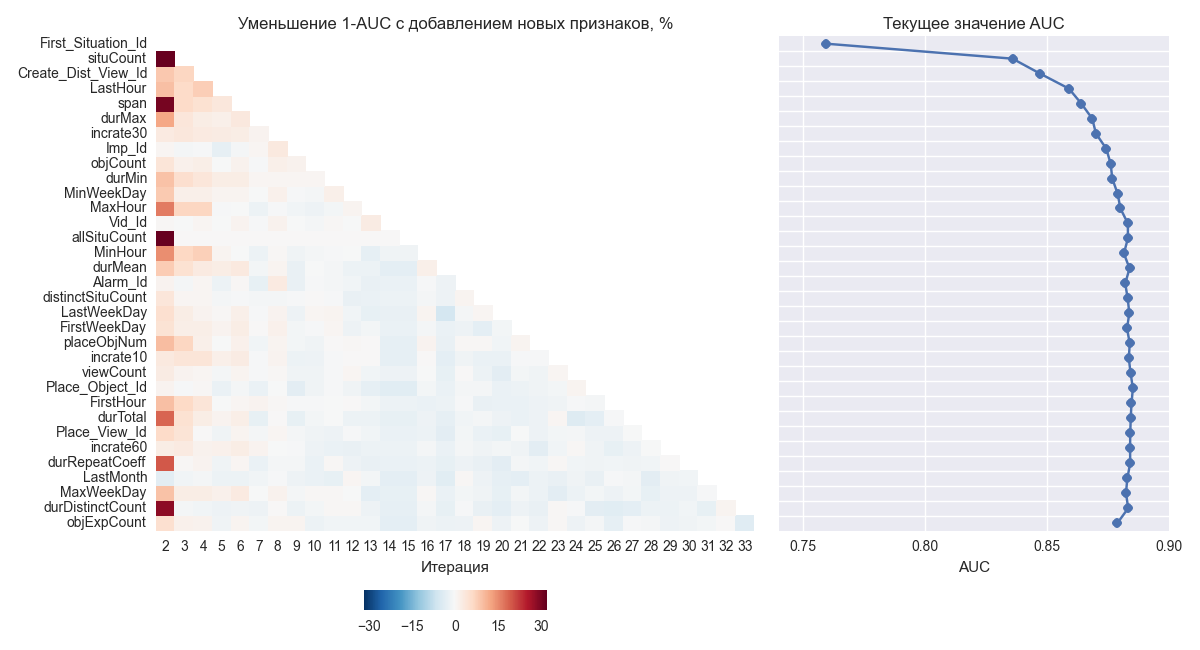
\includegraphics[width=\textwidth]{fullAdaptiveData.png}
\end{figure}


\begin{table}
\label{tbl:adaptiveAdditionScores}
\caption{Наиболее эффективные признаки, в порядке включения в модель.}
\begin{tabular}{ l p{7cm} l}
  \toprule
  \cyrins{\textbf{Признак}} & \cyrins{\textbf{Описание}} & \cyrins{\textbf{Тип, число значений}} \\ 
  \midrule
  {\texttt First\_Situation\_id} & Тип первой ситуации в инциденте & Категориальный, $\sim$600\\ 
  {\texttt situCount} & Количество ситуаций в инциденте & Количественный\\ 
  {\texttt Create\_Dist\_View\_id} & Дистанция (место) инцидента & Категориальный, 22  \\  
  {\texttt LastHour} & Час последней ситуации в инциденте & Количественный \\ 
  {\texttt span} & Продолжительность инцидента от начала первой до начала последней ситуации & Количественный \\ 
  {\texttt durMax} & Максимальная продолжительность ситуации в инциденте & Количественный \\ 
  {\texttt Place\_Object\_Id} & Идентификатор отказавшего объекта, на котором возникла первая ситуация   & Категориальный, $\sim$65000  \\
  {\texttt incrate30} & Количество инцидентов, зарегистрированных на объекте в пределах 30 мин до регистрации инцидента  & Количественный  \\
  {\texttt imp\_id} & Степень важности инцидента & Категориальный, 4 \\
  {\texttt objCount} & Количество объектов, затронутых инцидентом & Количественный \\
  {\texttt durMin} & Минимальная продолжительность ситуации в инциденте & Количественный\\
  {\texttt MinWeekDay} & Минимальное значение дня недели среди ситуаций инцидента & Категориальный, 7  \\
  {\texttt MaxHour} & Максимальное значение часовой компоненты среди ситуаций инцидента & Категориальный, 24 \\
  {\texttt Vid\_id} & Идентификатор вида инцидента & Категориальный \\
  \bottomrule
\end{tabular}
\end{table}

\todo{Анализ важности признаков с помощью их последовательного жадного добавления: на каждой итерации к текущему набору признаков, начиная с {\texttt First\_Situation\_id}, добавляется новый признак, при котором точность ранжирования увеличивается сильнее всего. Рис.~\ref{fig:dynamics}  На диаграмме слева показаны относительные изменения величины $1-\textrm{AUC}$ при добавлении каждого из признаков, не входящих в текущий набор. График справа показывает динамику точности предсказательной модели, построенной по текущему набору признаков. Таблица~\ref{tbl:adaptiveAdditionScores} Несколько первых признаков, до насыщения модели.}

\subsection{Анализ эффективности признаков}\label{sec:greedy}
На рис. \ref{fig:adaptiveAdditionScores} показаны результаты эксперимента по последовательному адаптивному добавлению в модель новых признаков. На каждом шаге для каждого из еще не входящих в модель признаков совершается пересчет точности модели с этим дополнительным признаком; тот, для которого наблюдается наибольшее приращение точности, включается в модель. В общей сложности рассматривается 34 признака, процедура начинается с признака типа первой ситуации (как наиболее информативного). 

В левой части рисунка \ref{fig:adaptiveAdditionScores}(a) показаны относительные изменения характеризующей ошибку величины $1-\text{AUC}$ для каждой итерации (горизонтальная ось) и каждого признака--кандидата (вертикальная ось). Признаки упорядочены post factum по очередности включения в модель, так что диаграмма имеет треугольный вид. В правой части рисунка показаны значения AUC соответствующей модели для каждой итерации. Для ускорения процедуры, модели в этом эксперименте строились с уменьшенным числом деревьев, поэтому их значения AUC ниже значения, указанного для основной модели на рис. \ref{fig:ROCcurves}. 

В результате данного эксперимента мы видим, что модель насыщается после включения в нее 10 -- 15 признаков, и ее точность перестает существенно меняться, если не считать небольшого эффекта переобучения, наблюдаемого в конце эксперимента. Первые несколько признаков являются одновременно достаточно информативными и разнообразными; их описания приведены в таблице \ref{fig:adaptiveAdditionScores}(b). На левой части рис. \ref{fig:adaptiveAdditionScores}(a) хорошо видно, что полезность признаков падает с итерациями, причем падение является резким в моменты, когда в набор включается признак, родственный рассматриваемому (см., например, \texttt{span} и \texttt{situCount}). Несмотря на это, мы видим, что полезно иметь, например, много разных признаков, характеризующих время ситуаций.

\nomenclature{АПК-ДК}{Аппаратно-программный комплекс диспетчерского контроля}

\begin{figure}[thb] 
\centering
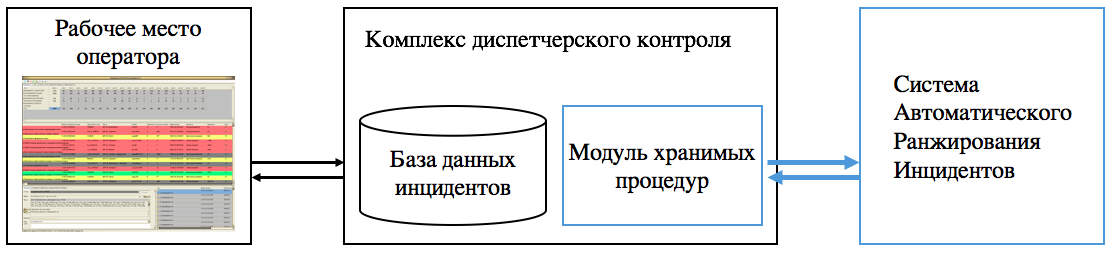
\includegraphics[width=13cm]{modules-v2}
\centering
\caption{Схема интеграции САРИ и АПК ДК.}
\centering
\label{fig:modules}
\end{figure}

\begin{figure*}[thb] 
\centering
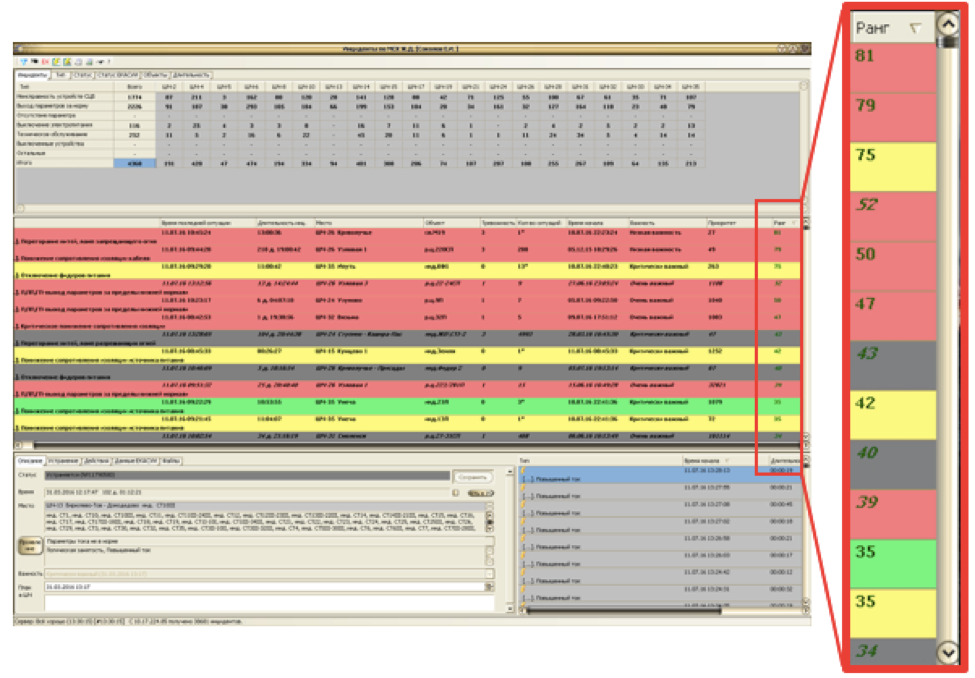
\includegraphics[width=11cm]{ui}
\caption{Отображение результатов ранжирования в пользовательском интерфейсе инженера службы мониторинга.}
\centering
\label{fig:ui}
\end{figure*}

\nomenclature{АРМ}{Автоматизированное рабочее место}

\section{Опыт внедрения}
Построенная модель ранжирования инцидентов была интегрирована в виде нового элемента, АПК «САРИ» (Система автоматического ранжирования инцидентов), в комплекс диспетчерского контроля ЦУСИ РЖД. \nomenclature{САРИ}{Система автоматического ранжирования инцидентов}  Схема интеграции и взаимодействующие модули представлены на рис. \ref{fig:modules}. 

Модуль ранжирования инцидентов выполняется на изолированном сервере. Он синхронно опрашивает модуль хранимых процедур в базе данных инцидентов на предмет обновления полей инцидентов и при необходимости инициирует пересчет при получении новых инцидентов и ситуаций. Важно отметить, что не все поля данных могут быть получены в оперативном режиме.

При получении новых данных, модуль осуществляет ранжирование инцидентов по набору исходных признаков и выдает прогнозное значение. Это значение далее отображается в виде отдельного столбца в интерфейсе инженера службы мониторинга с возможностью сортировки, см. рис. \ref{fig:ui}. Предсказательная модель выдает обновленное ранжирующее значение за 1.2 миллисекунды. Для удобства восприятия операторами, ранги инцидентов выдаются в виде целых чисел из интервала $[0,100]$ и соответствуют интервалу вероятностей $[10^{-6},1]$ на логарифмической шкале.


На исторических данных построено решающее правило, лес из 4000 решающих деревьев глубины 10.  Итоговое правило имеет 300,549 вариантов исходов и включает в себя более 3 лет исторических данных (5.3 млн инцидентов).

За время подконтрольной эксплуатации системы (май--июнь 2016 года, 1 месяц) в ней было зарегистрировано 581 032 ситуаций, объединенных в 92 339 инцидентов. Среди них предотказами было признано 2187 инцидентов. %Среднее время ответа САРИ – 1.7 мс. 
Точность модели в тестовой эксплуатации оказалась очень близка к предварительной оценке на тестовой выборке (AUC 0.901 и 0.904, соответственно).

\begin{figure}
\centering
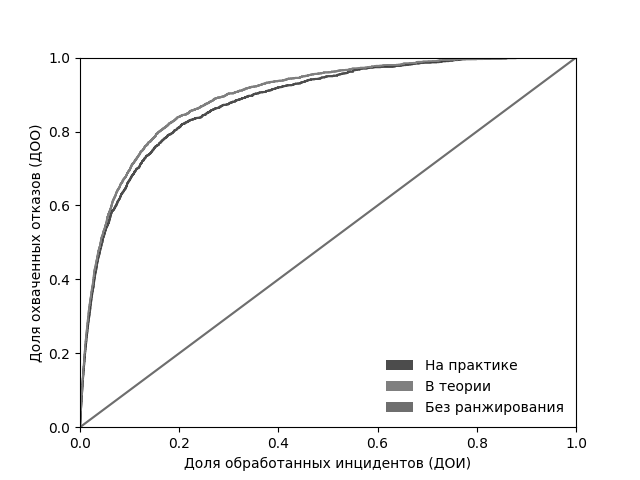
\includegraphics[width=9cm]{image19}
\caption{Операционная характеристика функции ранжирования (в теории и на практике)}
\centering
\label{fig:image19}
\end{figure}

На практике была показан режим работы, при котором для захвата 80\% предотказов достаточно охватить 20\% общей массы инцидентов в системе. Оценка снижения времени реакции инженера мониторинга на предотказ - до 5 раз (см. Рис. \ref{fig:ROCcurves}).

Модель полезно периодически обновлять, чтобы учитывать свежие данные. На графике ниже показано улучшение при обновлении раз в квартал.



\section{Обсуждение}
Нами была разработана и внедрена основанная на машинном обучении модель автоматического ранжирования инцидентов, регистрируемых устройствами ЖАТ на Московской железной дороге. Модель позволяет инженерам Центра управления инфраструктурой оперативно оценивать вероятности отказов и предотказных состояний и сокращает время реакции и устранения неполадок. Нами продемонстрирована высокая точность ранжирования с помощью построенной модели. Нам представляется полезным и перспективным более широкое внедрение предложенной нами технологии в системах железнодорожного мониторинга.  

Отметим два возможных направления развития данного проекта. Во-первых, как обсуждалось в разделе \ref{sec:stat}, разработанная нами модель является чисто статистической и не учитывает различия в важности разных отказов и предотказных состояний. Было бы полезно дополнить нашу модель достаточно точной программной моделью потерь как функции отказа. Математически это можно выразить следующим образом. Имеющаяся модель оценивает условную вероятность отказа или предотказного состояния при наличии инцидента с определенными характеристиками: $\mathbb P(\text{предотказ}|\text{инцидент})$. Практически более полезной была бы оценка условного математического ожидания потерь (например, в денежном выражении) при наличии данного инцидента: $\mathbb E(\text{потери}|\text{инцидент})$. Если считать, что потери происходят только при предотказе, то $\mathbb E(\text{потери}|\text{инцидент})=\mathbb E(\text{потери}|\text{предотказ})\cdot\mathbb P(\text{предотказ}|\text{инцидент})$, то есть для оценки $\mathbb E(\text{потери}|\text{инцидент})$ нам необходимо перемножить разработанную нами оценку вероятности предотказа на ожидаемые потери в случае предотказа, $\mathbb E(\text{потери}|\text{предотказ})$. Оценка этой последней величины может быть либо задана явно в соответствии с существующими регламентами, либо, при наличии хорошо структурированных и достаточно полных исторических данных о потерях, получена посредством их анализа с помощью методов, аналогичных применявшимся в настоящей работе.

Другим возможным направлением развития проекта является более глубокий анализ инцидентов, возможно с привлечением более детальной информации о предотказных ситуациях. Имеющаяся в основной исторической базе данных информация об инцидентах часто довольно скудна, например если инцидент состоит лишь из одной ситуации, описывающей повышение напряжения, то вся доступная информация об этом событии ограничивается указанием соответствующего временного интервала. В то же время можно ожидать, что дополнительная информация, скажем, о максимальном значении напряжения, скорости его изменения и т.п., позволила бы уточнить прогноз наличия предотказного состояния.


Опыт применения методов машинного обучения к задачам управления инфраструктурой российских железных дорог на Московской железной дороге позволяет ожидать положительные практические результаты при дальнейшем развитии и тиражировании достигнутых с совместной рабочей группой специалистов Московской дирекции инфраструктуры Московской железной дороги научных и практических успехов.

При дальнейшем развитии системы вести в xgboost-модель дополнительные признаки, отражающие историю аналогичных инцидентов/ситуаций на данном участке.

По результатам данной работы, ученый совет ОАО «РЖД» признал перспективным применение современных методов машинного обучения к задачам управления инфраструктурой российских железных дорог и порекомендовал продолжить развитие, разработку и внедрение системы. 

Представленные наработки в области интеллектуального анализа данных также рекомендовано апробировать в других областях железнодорожного транспорта.
           % Глава 2
\chapter{Применение обучения с подкреплением для распределения радиоресурсов в гетерогенных сетях малых станций} \label{chapt2}

\section{Введение} \label{sect2_1}

Растущий спрос на поддержание высокого качества услуг беспроводных сотовых технологий создает реальную проблему для телекоммуникационных сетей новых поколений~\cite{TS36.300}. Одним из основных технических требований, предъявляемых к современным сотовым системам, является максимизация фактора повторного использования частот ~\cite{M.1645}. Дефицит лицензированного спектра безусловно приводит к перекрытию диапазонов частот и интерференции между сотами (Inter-Cell Interference, ICI). В сфере контроля и ликвидации интерференции осуществляется интенсивная научная деятельность. В промышленности эти усилия в основном отражаются в виде строгого статического разделения частот или реактивного (в отличие от активного) ручного управления доступным спектром.

Концепция малых сот считается одним из самых практичных способов увеличения общей пропускной способности системы. В этом подходе большое количество маломощных устройств (малые соты) используется для увеличения повторного пространственного использования частот и улучшения местного покрытия. Согласно определению консорциума Small Cell Forum, «малые соты — это управляемые оператором маломощные беспроводные точки доступа с интеллектуальным обслуживанием, работающие в лицензированном диапазоне радиочастотного спектра. К типам малых сот относятся фемтосоты, пикосоты, метросоты и микросоты. Размер сот увеличивается от фемтосот (наименьший) до микросот (наибольший)»~\cite{6171992}. Довольно часто малые соты развертываются без или с небольшим объемом радиопланирования от оператора сети. Для того, чтобы гарантировать в этом случае некоторый заданный уровень качества обслуживания, необходимо внедрять интеллектуальные механизмы управления радиоресурсами для малых сот. Эта концепция принципиально изменяет требования к работе системы сотовых сетей выбиваясь из традиционных представлений о структуре сетей сотовой связи ~\cite{6211486}. При использовании этого подхода большое количество маломощных устройств разворачивается с целью увеличения коэффициента повторного использования частот на выделенной области покрытия. В дополнение к обширному уплотнению, устройства теперь могут часто включаться и выключаться, что вызывает частые неконтролируемые изменения в структуре сети. Таким образом, применение традиционные подходов к контролю интерференции перестало быть возможным, поскольку они основаны на предположении о равномерном гексагональном построении сети и подходят только для централизованного управления базовыми станциями.

Вместе с ростом числа устройств увеличивается количество накладных расходов на передачу управляющей информации. В таких условиях использование централизованных решений становится гораздо менее эффективным, а распределенные алгоритмы для управления ресурсами являются более перспективными. Эффективное управление радиоресурсами и координация интерференции являются неотъемлимыми механизмами для успешного внедрения гетерогенных сетей с малыми сотами.   

В этой главе мы предлагаем подход к управлению передачами на базовых станциях, динамическую схему распределения ресурсов с распределенной двухуровневой процедурой обучения. Мы предполагаем использование только локальной информации с ограничением обмена информацией между соседними сотами. По замыслу, на каждой соте должен быть выработан уникальный набор правил распределения ресурсов, позволяюший всей системе оперативно прийти к оптимальной конфигурации. Мы иллюстрируем применение этой стратегии обучения для задачи выделения частотных поддиапазонов. Каждый обучаемый агент исследует окружающую среду, изучая реакции от конкурирующих агентов и невзаимодействующих базовых макро станций. Полученная информация затем используются, чтобы выбрать наиболее подходящее расписание передач. 

Предлагается рассмотреть распределенную мультиагентную стратегию, где малые соты локально контролируют использование ресурсов для максимизации общей пропускной способности системы. Основная идея заключается в том, чтобы возложить на каждую базовую станцию принятие решение об использовании радиоресурсов. При принятии решения должна учитываться занятость ресурсов окружающих сот. Основной вклад данной работы заключается в следующем. Предложен новый метод для координации интерференции в плотных гетерогенных сетях. Рассмотрены две типичные проблемы часто возникающие в параллельных схемах обучения - разрастание обучаемой модели и блокирование возможности обследования. Предложенный алгоритм осуществляет мониторинг местного уровня интерференции, использование ресурсов и выделяет блоки физических ресурсов оптимальным образом. Алгоритм является полностью распределенным, предполагается отсутствие связи между сотами. Алгоритм быстро адаптируется к изменению интерференции и внешних условий сети, что делает его очень практичным. Дополнительно изучается вопрос о скорости сходимости распределенного механизма и предлагается ряд промежуточных процедур для повышения эффективности обучения. Сходимость и быстродействие алгоритма исследуется путем имитационного моделирования. Результаты предложенного метода оцениваются при помощи моделирования для сети базовых станций LTE и сравниваются с рядом традиционных схем распределения ресурсов. Результаты моделирования на системном уровне показывают, что она обеспечивает значительное улучшение производительности системы для разнородного внедрения с невзаимодействующими агентами без ущерба для эффективности системы в целом.

\section{Описание технологии радиодоступа} \label{section2_2}


\subsection{Архитектура базовой станции} 
Ключевым элементом сети LTE, отвечающим за эффективное использование частотного спектра, является базовая станция. В данном разделе представлена архитектура базовой станции и рассмотрены компоненты, участвующие в процессе управления ресурсами.

\begin{figure}
  \center
  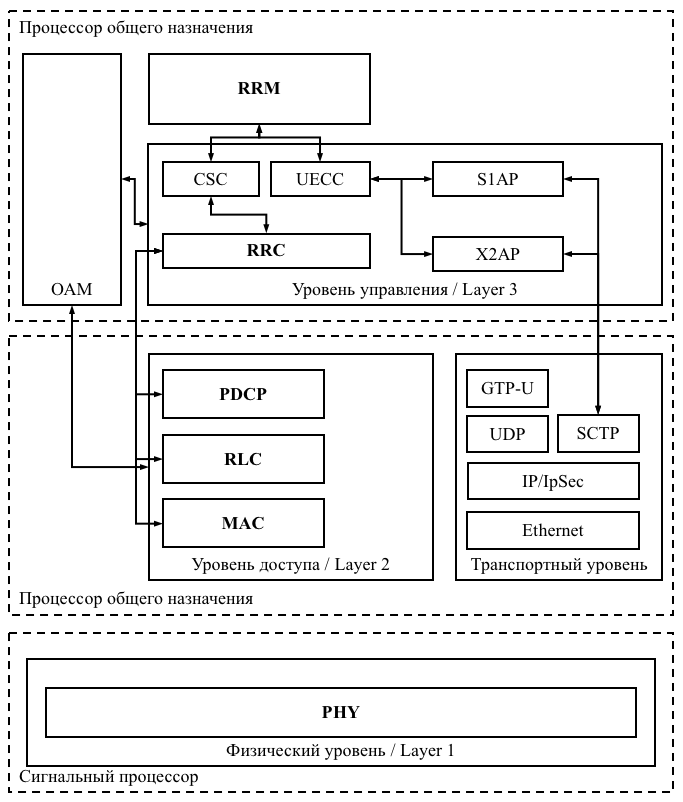
\includegraphics [width=\textwidth]{image7}
  \caption{Архитектура базовой станции LTE. Источник \cite{Aricent}} 
  \label{img:image7}  
\end{figure}


Протокол PDCP (Packet Data Convergence Protocol) обеспечивает компрессию заголовков (ROHC), шифрование, сохранение порядка следования пакетов.

Протокол RLC (Radio Link Control) выполняет функции сегментирования, отброса дубликатов и сохранение порядка следования пакетов \cite{access2008and}. RLC функционирует в одном из трех режимов передачи: прозрачный (transparent mode, TM), передача без подтверждения (unacknowledged mode, UM) и передача с подтверждением (acknoledged mode, AM). В режиме AM поддерживаются специальные функции для повторной передачи данных.

Протокол RRC покрывает следующие функциональные области: передача системной информации, управление RRC соединением (RRC connection control). Сюда относятся процедуры создания, изменения и удаления RRC соединения, пейджинг, активацию защиты соединения, контроль ресурсов для передачи пользовательских данных. Также к этой области относится процедура хэндовера (handover) и конфигурация более низких уровней (PDCP, RLC, MAC).

Протокол RRC также осуществляет настройку измерений качества канала и отчетность на стороне пользовательского устройства, включая настройку и активацию периодов измерений (см. раздел \ref{ch_estimation}). Актуальность информации о состоянии канала напрямую влияет на эффективность передачи пользовательских данных.

Задача управления радиоресурсами решается протоколом RRM (Radio Resource Management). Сюда входит динамическое распределение ресурсов в восходящих и нисходящих направлениях, принятие решений о необходимости хэндовера и допуска пользователей к обслуживанию. Блок RRM также отвечает за ограничение использования спектра с целью контроля интерференции между базовыми станциями.

Задача протокола MAC (Media Access Control) заключается в выделении пользователям частотно временных ресурсов и поддержании гарантий качества обслуживания. Блок MAC также осуществляет выбор сигнально-кодовой конструкции, используемой для обслуживания пользователей.

\subsection{Физический уровень LTE} %\label{section5_2}

Обмен между базовой станцией и абонентским устройством осуществляется кадрами (в терминологии LTE – радиокадр) длительностью 10 мс (см. рис. \ref{img:image8}). Стандарт предусматривает две структуры кадров. Одна для случая частотного разделения каналов (Frequency Division Duplex — FDD), другая - для временного (Time Division Duplex — TDD).

В LTE используется OFDM модуляция, хорошо исследованная при разработке систем DVB, Wi-Fi и WiMAX. В стандарте LTE установлен стандартный шаг между поднесущими ∆f = 15 кГц, что соответствует длительности OFDM-символа 66,7 мкс.

Все временные параметры в спецификации LTE привязаны к минимальному временному кванту $T_s   =  1/(2048 ∙ ∆f)$, где ∆f – шаг между поднесущими, стандартно – 15 кГц. Таким образом, длительность радиокадра – $307200 ∙ T_s$. Отметим, что квант времени соответствует тактовой частоте 30,72 МГц, что кратно стандартной в 3G-системах частоте обработки 3,84 МГц (8×3,84 = 30,72) \cite{access2010lte}.

\begin{figure}
  \center
  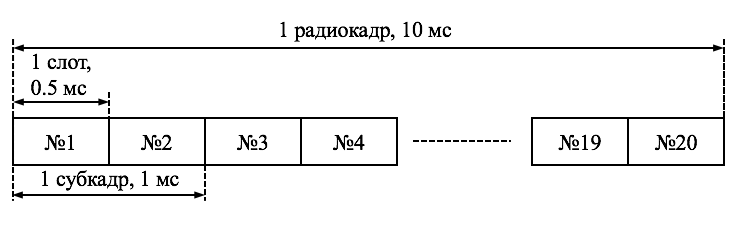
\includegraphics [width=\textwidth]{image8}
  \caption{Структура кадра LTE. Источник \cite{вишневский2009технология}} 
  \label{img:image8}  
\end{figure}


В каждом слоте абонентскому устройству назначается определенный диапазон канальных ресурсов в частотно-временной области – ресурсная сетка (см. рис. \ref{img:image9}). Ячейка ресурсной сетки (ресурсный элемент) соответствует одной поднесущей в частотной области и одному OFDM-символу – во временной. Группа ресурсных элементов образует ресурсный блок. Ресурсный блок – это минимальный квант радиоресурса, выделяемый абонентскому устройству планировщиком базовой станции. Ресурсный блок занимает 12 поднесущих (т.е. 180 кГц) и 7 или 6 OFDM-символов, в зависимости от типа циклического префикса – так, чтобы общая длительность слота составляла 0,5 мс. Число ресурсных блоков в ресурсной сетке зависит от ширины полосы канала и составляет от 6 до 100 (ширина частотных полос восходящего/нисходящего каналов в LTE – от 1,4 до 20 МГц). В новой версии стандарта LTE-A добавлена возможность агрегации до 5 полос шириной 20 МГц \cite{access2013lte}. О распределении ресурсов в каждом слоте базовая станция сообщает в управляющем канале, располагающемся в начале каждого субкадра.

\begin{figure}
  \center
  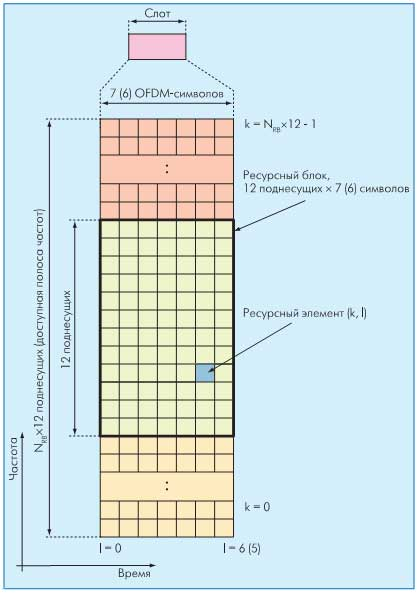
\includegraphics [width=0.9\textwidth]{image9}
  \caption{Ресурсная сетка LTE при стандартном шаге поднесущих ∆f = 15 кГц. Источник \cite{вишневский2009технология}} 
  \label{img:image9}  
\end{figure}

Поднесущие модулируются посредством 4-, 16- и 64-позиционной квадратурной фазово-амплитудной модуляции (QPSK, 16-QAM или 64-QAM). Соответственно, один символ на одной поднесущей содержит 2, 4 или 6 бит информации. При стандартном префиксе символьная скорость составит 14000 символов/с. Сигнал с полосой 20 МГц содержит 100 ресурсных блоков или 1200 поднесущих, что дает общую скорость в канале от 33,6 до 100,8 Мбит/с.

Для повышения надежности передачи на физическом уровне стандарт LTE использует механизм HARQ (Hybrid Automatic Repeat Request). HARQ представляет собой комбинацию высокоскоростного помехоустойчивого кода и стандартного механизма ARQ \cite{access2008and}. Эта технология позволяет пользовательскому устройству запросить дополнительные проверочные биты при обнаружении ошибки декодирования.

\subsection{Оценка канала} \label{ch_estimation}

Для эффективного осуществления передачи данных базовая станция должна иметь оценку качества канала до обслуживаемого пользователя. Эта оценка используется для планирования расписания передач. Стандарт LTE предусматривает возможность запросить у пользователя отчет с оценкой качества канала. Для того чтобы задать формат отчетов о качестве канала, базовая станция посылает пользователю служебное сообщение RRC ConnectionReconfiguration \cite{access2012lte} с указанием следующих параметров:

При получении сообщения RRC ConnectionReconfiguration \cite{access2012lte} пользовательское устройство проводит измерения мощности пилотных сигналов соседних станций и через время равное reportInterval посылает их в отчете Measurement report. Эти величины называются RSRP (Reference Signal Received Power) \cite{access2010lte} и квантуется в соответствии с рисунком 10.

\section{Обзор методов координации интерференции в сотовых сетях}
%\blindtext

В данном разделе представлен обзор смежных работ в области управления радиоресурсами и координации интерференции в сотовых сетях. Существует множество исследований по данной теме, в особенности, на тему интерференции между макростанциями. На данный момент этот эффект является одним из основных сдерживающих факторов в сценариях с плотным развертыванием малых сот. В связи с этим в мире ведутся многочисленные исследовательские работы, посвященные различным вариантом управления ресурсами в разнородных сетях. Подробный обзор основных методов управления интерференцией, совместимых с LTE представлен в ~\cite{cite_overview}.


%NEW SECTION
%======================================================
\subsection{Методы частотного разделения} \label{sect4_1}

За последние 40 лет проблеме повышения производительности сетей сотовой связи было посвящено множество исследовательских работ. В данном разделе представлен общий обзор направлений современных исследований в данной области.

Как правило, среди алгоритмов повторного использования частот выделяют:
\begin{itemize}
\item Полное повторное использование частот (Full Frequency Reuse), когда вся полоса полностью используется каждой сотой независимо от местоположения абонентов. Распределение ресурсных блоков в этом случае осуществляет планировщик базовой станции, а информацию о распределении ресурсов базовая станция сообщает абонентским станциям по специальному управляющему каналу.
\item Жесткое повторное использование частот (Hard Frequency Reuse), когда вся полоса частот разделена на фиксированное количество полос, которые назначаются сотам в соответствии с частотным планом сети (см. рис. \ref{img:image11}).

\begin{figure}[ht] 
  \center
  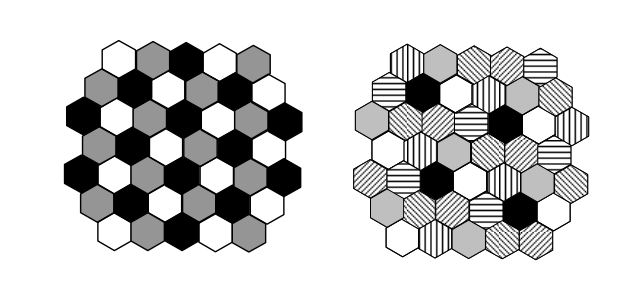
\includegraphics {image11}
  \caption{Схема распределения частотных каналов между сотами ($$N = 3, N = 7$$)} 
  \label{img:image11}  
\end{figure}


\item Мягкое повторное использование частот (Soft Frequency Reuse — SFR), когда площадь, обслуживаемая базовой станцией, разделяется на две зоны — центральную, в которой абонентским устройствам доступны все частотные ресурсы и зону, находящуюся на границе, в которой устройствам доступна только часть ресурсов. Отсутствие частотных ресурсов на границе соты, может привести к существенному уменьшению пропускной способности в канале. Поэтому на частотах, используемых устройствами на границе, повышается мощность передачи, чтобы увеличить отношения SINR, а значит и значение пропускной способности (см. рис. \ref{img:image12}).
\end{itemize}

\begin{figure}[ht] 
  \center
  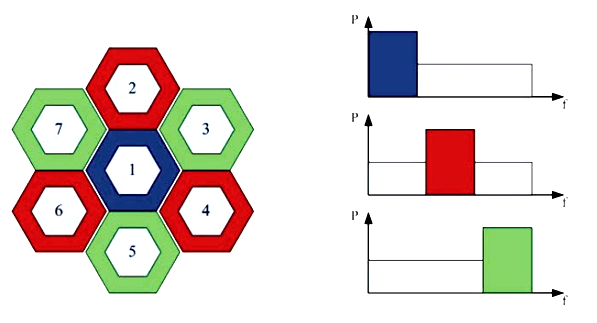
\includegraphics {image12}
  \caption{Схема использования частот и профили мощности для метода SFR} 
  \label{img:image12}  
\end{figure}

Одна из первых статей, описывающих динамическое назначение каналов (Dynamic Channel Allocation — DCA) для сетей с коммутацией каналов была представлена в 1971 году \cite{cox1971dynamic}. Для осуществления вызова устройству на время разговора назначался канал из стека доступных каналов. После завершения разговора, канал возвращается в общий стек. Чтобы избежать помех, канал, который используется в одной соте мог быть назначен одновременно в другую соту, только если расстояние между двумя сотами было больше, чем минимальное расстояние повторного использования.

Помимо DCA, в то же время появилась схема заимствования каналов (Borrowing Channel Assignment — BCA), которая была предложена в работах \cite{engel1973statistically1}, \cite{engel1973statistically2} и \cite{electosvyasru-2017}. В отличие от схемы DCA, где соты могли использовать все каналы, BCA сначала фиксирует каналы, а затем позволяет загруженным сотам заимствовать у соседних сот неиспользуемые каналы. На рисунке \ref{img:image13} показана возможность использования незанятых каналов, доступных белым сотам, серой сотой, указанной стрелкой.

\begin{figure}[ht] 
  \center
  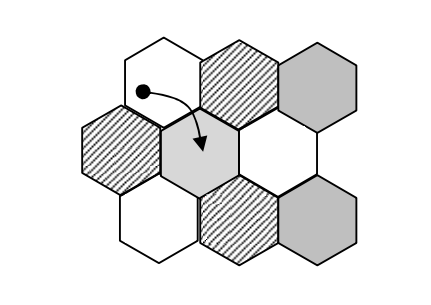
\includegraphics {image13}
  \caption{Схема заимствования каналов BCA. Источник \cite{engel1973statistically1}} 
  \label{img:image13}  
\end{figure}

Отметим, что если динамическое назначение каналов на базовой станции осуществляется независимо от решения соседних базовых станций, то для эффективной борьбы с интерференцией станция должна иметь возможность измерения уровня интерференции в канале передачи.

Для динамической координации интерференции в LTE между базовыми станциями поддерживается сигнализация через специфицированный интерфейс X2 \cite{network2008x2}.

Данный интерфейс позволяет напрямую между станциями обмениваться сообщениями, такими как: индикатор мощности передачи ресурсных блоков RNTP – Relative Narrowband Tx Power, индикатор высокого уровня интерференции HII – High Interference Indicator, и индикатором перегрузки OI – Overload Indicator.

RNTP - двоичный индикатор, каждый бит которого указывает, превышает ли мощность передачи соответствующего частотного блока некоторое пороговое значение. С помощью RNTP базовая станция информирует своих соседей о том, с какой мощностью будут излучаться все частотные блоки на длительности одного или нескольких кадров.

HII - двоичный индикатор, каждый бит которого указывает на предстоящую передачу в определенных частотных блоках в восходящем канале, которая может увеличить уровень интерференции на соответствующих ресурсах.

OI – индикатор, который отражает уровень интерференции (низкий, средний, высокий), на частотных блоках восходящего канала.
Другая техника — Reuse Partitioning. Этот алгоритм является разновидностью статического планирования и нацелен на увеличения пропускной способности путем использования различных методов совместного использования частот для конкретного пользовательского устройства. Впервые этот алгоритм представлен в 1983 году \cite{halpern1983reuse}, под названием Reuse Partitioning. В последствие, в конце 90-x он был заново открыт как Intelligent Underlay-Overlay \cite{ling1996capacity}, \cite{wille1996capacity}, \cite{nielsen1997capacity}, \cite{wigard1997improved}. Сейчас, благодаря работе WiMAX форума и консорциума 3GPP, этот алгоритм известен как алгоритм частичного повторного использования частот, Fractional Frequency Reuse — FFR \cite{wimax2006technical}.

Алгоритм FFR разделяет полосу частот на две группы — внутреннюю и внешнюю. Внутренняя полоса частот назначается для передачи на пониженной мощности устройствам, расположенным близко к обслуживающей базовой станции. Для устройств, находящими на границе соты, выделяется внешняя полоса с коэффициентом повторного использования большим единицы.

В то время как reuse partitioning и intelligent underlay-overlay в большей степени известны как алгоритмы разделения частот в сетях с коммутацией каналов, FFR чаще используется в сетях с пакетной коммутацией.

Обобщение алгоритма FFR было предложено в работах \cite{bonald2005inter}, \cite{bonald2006inter}. Алгоритм работает с произвольными участками внутри соты, в каждом из которых пользовательское устройство обслуживается с определенным профилем передачи (transmission profile). Профиль представляет собой определенной набор активных передатчиков. Аналогичные исследования описаны в работе \cite{liu2006inter}.

Алгоритм динамической локальной координации (dynamic local coordination) представлен в работе \cite{sternad2003attaining}. Данный алгоритм основан на использовании общего планировщика между секторами внутри одной соты и разных коэффициентов повторного использования частот, для устройств, в зависимости от расстояния до обслуживаемой базовой станции. На основе этой работы, в статье \cite{necker2007local}, проведена всесторонняя оценка производительности алгоритмов.

Гибридные и децентрализованные схемы координации интерференции были предложены компанией Alcatel-Lucent в работах \todo{[37-39]} \cite{R1-050407,R4-092042,R1-081873} и оказались особенно эффективны для балансировки нагрузки сот.

Исследователи из Nortel в работах [40], [41] и [42] предлагают адаптивную схему повторного использования частот (Adaptive Fractional Frequency Reuse — AFFR), основанную на подходах FFR и SFR, которая также относится к гибридным децентрализованным схемам координации интерференции. Согласно алгоритму AFFR сота может работать в одном из четырех режимов, которые различаются различными политиками совместного использования частот. Первый режим предполагает передачу на полной мощности во всем доступном частотном диапазоне. В противоположность первому режиму четвертый режим предполагает разделение частотного диапазона на 3 части, аналогично HFR. Режимы 2 и 3 предполагают использование SFR с различными уровнями мощности. В данном алгоритме базовые станции могут взаимодействовать друг с другом и отправлять запросы на использование того или иного режима работы, если уровень интерференции становиться слишком высоким.

Исследователи из Texas Instruments в работах [43], [44] предлагают внести дополнения в подход FFR, так чтобы размер частотных блоков мог адаптивно настраиваться между сотами с помощью специального контроллера. Эта концепция представляет собой гибридную, децентрализованную схему координации интерференции.

Другие примеры распределенных схем представлены в работах \cite{rahman2008interference}\cite{li2006downlink}.

В работах [38] и [39] методы повторного использования частот в сетях с OFDMA анализируются на примере сетей LTE. Результаты моделирования в [39] показывают, что схемы с полным повторным использованием частот обеспечивает наилучший показатель пропускной способности, как для восходящего, так и для нисходящего канала, однако пользователи находящиеся на границе соты (cell edge users) испытывают высокий уровень интерференции и имеют приблизительно одинаковые показатели спектральной эффективности. В работе [38] показано, что спектральная эффективность пользователей, находящихся на границе соты, может быть увеличена с помощью использования схем согласованного частичного использования частот, в которой различные подканалы имеют различные уровни мощности передачи. Увеличение до 20 процентов в совокупной пропускной способности получено для схемы частичного повторного использования.

Математически, задачу назначения частотных диапазонов базовым станциям можно свести к задаче на графах. Алгоритмы, использующие теорию графов, как правило, представляют сеть в виде неориентированного графа, вершины которого обозначают базовые станции, а ребра – наличие интерференции между ними.

Одна из первых работ, авторы которой свели задачу назначения каналов к задаче раскраски графа, была представлена в 1980 году \cite{wimax2006technical}. Ранние работы по моделированию интерференции в сетях, основывались на моделях, использующих особый тип графов — граф единичных кругов \cite{bonald2005inter}, неориентированный граф, узлы которого является центрами единичных окружностей. Если пересечение двух окружностей не пусто, тогда соответствующие узлы соединяются ребром. Характерный вид unit disk graph представлен на рисунке \ref{img:image14}.

\begin{figure}[ht] 
  \center
  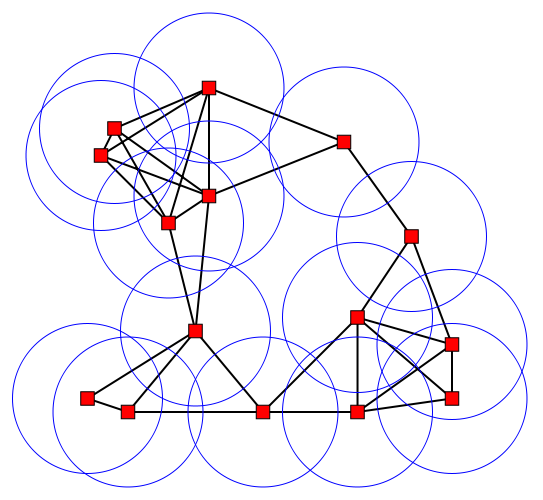
\includegraphics [width=10cm]{image14}
  \caption{Пример графа единичных кругов} 
  \label{img:image14}  
\end{figure}

Краткий обзор алгоритмов раскраски графов описан в работе \cite{bonald2006inter}. Большая часть работы посвящена обзору алгоритмов на гексагональных сетках. Также в работе рассмотрены результаты для unit disk graph. Изучению изменения характеристик сети вследствие ограничений, налагаемых введением честности между пользователями и профилем QoS, отражены в статье \cite{liu2006inter}. Иной подход к построению графов, предлагают работы, в которых вершины интерференционного графа представляют собой пользовательские устройства \cite{sternad2003attaining}.

С появлением децентрализованных сетей с пакетной коммутации в сотовой связи, схемы, основанные на взаимодействии между устройствами, становятся все более популярными. Теория игр исследует такие взаимодействия, поэтому ее методы были использованы для решения задач динамического назначения канальных ресурсов несколькими устройствами в ряде работ [42] и [43].

Другой поход к координации интерференции в сети представляет использование различных профилей мощности (Power Control). Исторически, Power Control использовался в сотовых сетях для решения проблемы, когда пользовательское устройство, находящееся на краю соты оказывается заглушенным устройствами, расположенными рядом с базовой станцией \cite{li2006downlink}, \cite{gilhousen1991capacity}. Это проблема решается ограничением мощности в восходящем канале, при постоянном уровне мощности на базовой станции. Такой подход, хотя и является не оптимальным с точки зрения общей пропускной способности или спектральной эффективности, но обеспечивает честность по отношению к пользователям, находящимся на границе соты.

Последние исследования для сетей 4-го поколения предлагают компромиссный подход, путем частичной компенсации потери мощности сигнала для пользователей находящихся на границе \cite{castellanos2008performance}, в отличие от полной, использовавшейся ранее. Частичная компенсация потери мощности сигнала обеспечивает улучшение общей пропускной способности на 20 процентов по сравнению с традиционными методами, если расстояние между базовыми станциями находится в промежутке от 500 м до 1 км, при ширине канала в 10 МГц. Для сценариев с небольшим межсотовым расстоянием, менее 500 м, частичная компенсация также показывает рост пропускной способности крайних пользователей (5-процентиль) на 10-15 процентов по сравнению с традиционными методами.

%NEW subSECTION
%======================================================
\subsection{Методы согласованной передачи} \label{sect4_2}
Технология MIMO (множественный вход – множественный выход) позволяет значительно увеличить помехоустойчивость каналов связи в условиях многолучевого распространения сигналов [49, 50]. Как правило, под аббревиатурой MIMO подразумевается целый ряд технологий:
\begin{itemize}
\item Использование, так называемых, «интеллектуальных» антенн (intelligent antennas), позволяющих формировать многолучевые диаграммы направленности. Данная технология позволяет увеличить эффективность использования спектра за счет передачи данных в параллельных лучах.
\item Использование пространственно-временного кодирования (Space-Time Coding – STC)
\item Использование поляризационного разделения каналов, поляризационной обработки сигналов.
\end{itemize}

Все разновидности технологии MIMO направлены на достижение одной цели – увеличение пиковой скорости передачи данных за счет увеличения соотношения сигнал/шум на приемном устройстве.

Наиболее широкое распространение получила технологи MIMO на основе пространственно-временного кодирования \cite{oestges2010mimo,3GPPTS2530,3GPPTR25814}, которая вошла в стандарты LTE 3GPP.

Алгоритмы координации интерференции в многоантенных системах были обобщены понятием сетевого MIMO (network MIMO, Net-MIMO, Cooperative MIMO, CO-MIMO или Ad-hoc MIMO), которое предполагает передачу или прием сигнала с помощью многоантенных систем на нескольких базовых станциях \cite{jindal2006mimo}. На нисходящем канале несколько базовых станций могут передавать по нескольким MIMO-путям одному и тому же пользовательском устройству. Аналогично, в восходящем канале сигналы от пользовательского устройства могут быть приняты одной или несколькими базовыми станциями.

\begin{figure}[ht] 
  \center
  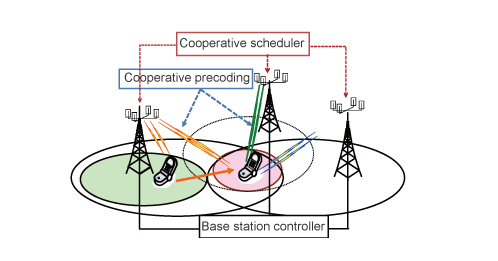
\includegraphics[width=15cm] {image15}
  \caption{Принципиальная схема организации сетевого MIMO} 
  \label{img:image15}  
\end{figure}


Одна из проблем реализации сетевого MIMO является задержка в ходе обмена информацией между базовыми станциями. В стандарте LTE минимальные задержки при обмене информацией между базовыми станциями с помощью интерфейса X2 составляют 20 мс. В то время как планирование ресурсов осуществляется каждую миллисекунду. Поэтому при обработке данных требуется учет этой особенности.

Технология координированной множественной передачи (CoMP) подразумевает обслуживание одного абонентского устройства несколькими базовыми станциями. Координированная передача и прием рассматриваются как способ, с помощью которого можно увеличить скорость передачи абонента, находящегося на границе соты. При этом повышение скорости передачи в нисходящем канале достигается за счет уменьшения уровня интерференции, а в восходящем канале - за счет параллельной обработки принятого сигнала на нескольких базовых станциях[55] .

В нисходящем канале можно выделить 2 основных метода кооперативной многоантенной передачи: совместная обработка (Joint Processing — JP) и координированное планирование (Coordinated Beamforming/Coordinated Scheduling — CB/CS). Оба метода представлены на рисунке \ref{img:image15}. В случае совместной обработки передаваемые данные доступны на всех базовых станциях, с которых ведется передача. Однако существует два различных варианта реализации этого подхода. В первом варианте осуществляется одновременная передача с нескольких базовых станций. А во втором варианте базовая станция, которая осуществляет передачу данных, выбирается динамически. То есть передача осуществляется только с одной базовой станции в каждый момент времени. При этом данные для передачи доступны на нескольких базовых станциях.

В случае координированного планирования передач данные всегда передаются только с одной базовой станции, при этом решение о расписании передач делается с учетом информации о планировании от нескольких соседних базовых станций \cite{karakayali2006network}, \cite{andrews2007overcoming}. При координированном приеме данных (т.е. при восходящей передаче) можно также выделить два различных варианта. Первый вариант — это совместный прием сигнала от пользовательского устройства на нескольких базовых станциях (Joint Reception — JR). Второй вариант - это координированное планирование передач с целью уменьшения или полного погашения интерференции. Кроме этого, возможна комбинация обоих названных вариантов.

%NEW subSECTION
%================================================
\subsection{Формирование диаграммы направленности} \label{sect4_3}
В последнее время, планирование ресурсов с возможностью формирования диаграммы направленности \cite{svedman2007opportunistic} является предметом пристального изучения.

В работе \cite{hu2008radio} исследована производительность системы связи, в которой применяется схема формирования диаграммы направленности антенн с псевдослучайной перестройки лучей (Organaized Beam Hopping — OBH). Сокращение интерференции в схеме OBH достигается путём пространственного разнесения передач от соседних базовых станций. Анализ производительности схемы OBH показал увеличение спектральной эффективности порядка 1 бит/с/Гц. Результаты были получены при помощи моделирования сотовой сети, состоящей из сот радиусом 1 км, каждая из которых имеет шесть лучей. В работах также отмечается ряд нерешенных вопросов, в том числе связанных с механизмом адаптации к различным профилям мобильного трафика.


%NEW subSECTION
%================================================
\subsection{Альтернативные подходы} \label{sect4_4}
Техника подавления помех (Interference Cancellation — IC), предложенная более 20 лет назад, хорошо известна в литературе, посвященной проблеме борьбы с интерференцией в беспроводных сетях. Основная концепция заключается в восстановлении сигналов помех, а затем вычитании их из принятого сигнала. Как правило, это предполагает хранение принятого сигнала в буфере для последующей обработки.

Подавление помех может применяться как на восходящем, так и нисходящем канале, но из-за сложности реализации, оно рассматривается, главным образом, как техника для восходящего канала и реализуется в приемнике базовой станции. Исчерпывающий обзор методов подавления помех, используемых в сотовых сетях, представлен в работе \cite{andrews2005interference}.
Dirty paper and sphere coding — это две последние инновации в алгоритмах кодирования, которые являются потенциально применимыми к сетям 4-го поколения.

Основная концепция Dirty paper coding заключается в предварительном кодировании каждого потока таким образом, что нужный сигнал отображается в некоторое кодовое слово. Приемник, обладающий знаниями о кодовом пространстве, может быть использован для успешного декодирования полезного сигнала в присутствии интерференции с помощью декодера \cite{choi2006capacity}.

Sphere coding еще один метод, которому уделяется большое внимание в качестве подхода для устранения помех. Суть подхода заключается в поиске N-мерной гиперсферы некоторого предопределенного радиуса R в кодовом пространстве. Выбор радиуса представляет собой компромисс между экспоненциально растущей сложностью поиска, с ростом R, и более высокой вероятностью ошибки при меньшем значении радиуса \cite{barbero2007performance}.

\subsection{Перспективные методы частотного разделения}

Для плотных неконтролируемых внедрений базовых станций задача управления интерференцией между сотами является более сложной, чем в традиционных операторских сотовых сетях. Один из перспективных методов управления радиоресурсами основывается на проведении предварительного исследовании радиоокружения, с целью выявления статистических данных об использовании ресурсов. Затем извлеченные данные могут быть использованы для непосредственного принятия решений (как в \cite{mab}) или (как, например, в \cite{q-learning}) для построения оптимальной схемы распределения ресурсов. В частности, в работе~\cite{q-learning} исследуется вопрос о самоорганизации и децентрализованном управлении интерференцией в сети фемтосот с целью разделения радиоресурсов между фемтосотами и макроокружением (сетью макро базовых станций и другими источниками интерференции). В этой работе рассмотрен многоагентный подход к обучению на основе распределенного Q-обучения (Q-learning). Малые соты меняют свою мощность передачи, чтобы максимизировать суммарную выходную мощность, в то время как суммарная интереференция макро пользователей в нисходящей линии связи поддерживается в заданных пределах.

В \cite{mp-qlearning} и \cite{fzq-learning} авторы предлагают другие схемы на основе Q-обучения и демонстрируют значительный выигрыш по сравнению с обычными методами повторного использования частот с точки зрения пропускной способности пользователей сотовой сети. Однако, эти методы устанавливают жесткие требования к качеству канала обратной связи и менее эффективны с точки зрения времени сходимости в динамичных случаях с гибким трафиком. 

В \cite{mab} предложен подход с использованием машинного обучения с подкреплением, где базовые станции автономно выбирают наиболее эффективную схему использования спектральных ресурсов из заранее заданного набора. Это позволяет гибко управлять компромиссом между фазой изучения окружающей среды и фазой использования накопленной информации. Похожие схемы с возможностью автоконфигурации и самооптимизации также были представлены в \cite{local-area}, где алгоритм позволяет сотам динамически выбирать начальные участки спектра и опирается на механизмы контроля мощности. Управление интерференцией между сотами было также изучено в \cite{on-uplink}, где авторы предложили схему планирования с фиксированными вероятностями выбора ресурсных блоков. В данном случае, сложность предлагаемых стохастически схем управления радио ресурсами является относительно низкой, поскольку они предполагают децентрализованный подход и требуют только ограниченный объем передачи управляющей информации. Однако, эти схемы могут быть неэффективными при рассмотрении сетей малых сот большого размера.
Еще один интересный децентрализованный подход был предложен в ~\cite{1666484}, где проблема распределения каналов сводится к задаче раскраски графа. Единственная информация, необходимая алгоритму, - обратная связь по уровню интерференции на выбранном канале. В~\cite{Duffy:2008:CAD:1377038.1377164} и ~\cite{4177619}сложность и скорость сходимости изучены для класса децентрализованных алгоритмов раскраски. Отметим, что проблема, рассматриваемая в данной главе, не может быть сведена к раскраске графа, так как соты могут находиться на одном и том же поддиапазоне, а границы частот поддиапазонов не фиксируются.
В то время как описанные решения обеспечивают подходы к управлению распределением ресурсов, они не учитывают ряд важных моментов, рассматриваемых далее в работе. Предлагается рассмотреть метод управления интерференцией, сделав упор на исследование нескольких ощутимых недостатков мультиагентного обучения. Основной проблемой является рассогласование между состоянием всей системы и поведением каждого агента в отдельности. В перспективе исследования скорости сходимости система имеет два состояния - состояние ''разведки'', где изучение окружающей среды движет систему к стабильному состоянию, и состояние ''эксплуатации'' - стабильное состояние, где эффективность обучения низка в связи с необходимостью сохранить стабильность системы. Недостатком такого подхода является то, что система интенсивно изучает среду в одном состоянии (где поведение агентов определяется, главным образом, исследованием поведения окружения), а затем работает в другом состоянии (определяемым эксплуатационным поведением агентов). В этой главе мы предлагаем первоначально заставить группу агентов вести себя уникальным образом, чтобы добавить больше смысла в процесс обучения. Мы также изучаем еще одну проблему схемы обучения, которая заключается в разрастании пространства состояний обучаемой модели с увеличением количества поддиапазонов.
Цель этого исследования заключается в получении схемы управления интерференцией посредством распределения частотных ресурсов с применением нескольких новых усовершенствований поведения обучаемых агентов с акцентом на их сосуществовании в плотной сотовой сети.


\section{Постановка задачи распределения ресурсов}
\subsection{Архитектура системы}
В этой главе мы рассматриваем сотовые сети технологии LTE/LTE-А с разнородным внедрением базовых станций, таких как макросоты и малые соты, как показано на Рис.~\ref{fig:architecture}. Малые соты обычно используются для улучшения покрытия в помещениях и для повышения общей пропускной способности в густонаселенных районах. Основной упор в данном разделе сделан на сосуществование малых сот с макросредой и некооперативными группами малых сот.

\begin{figure}
    \centering
    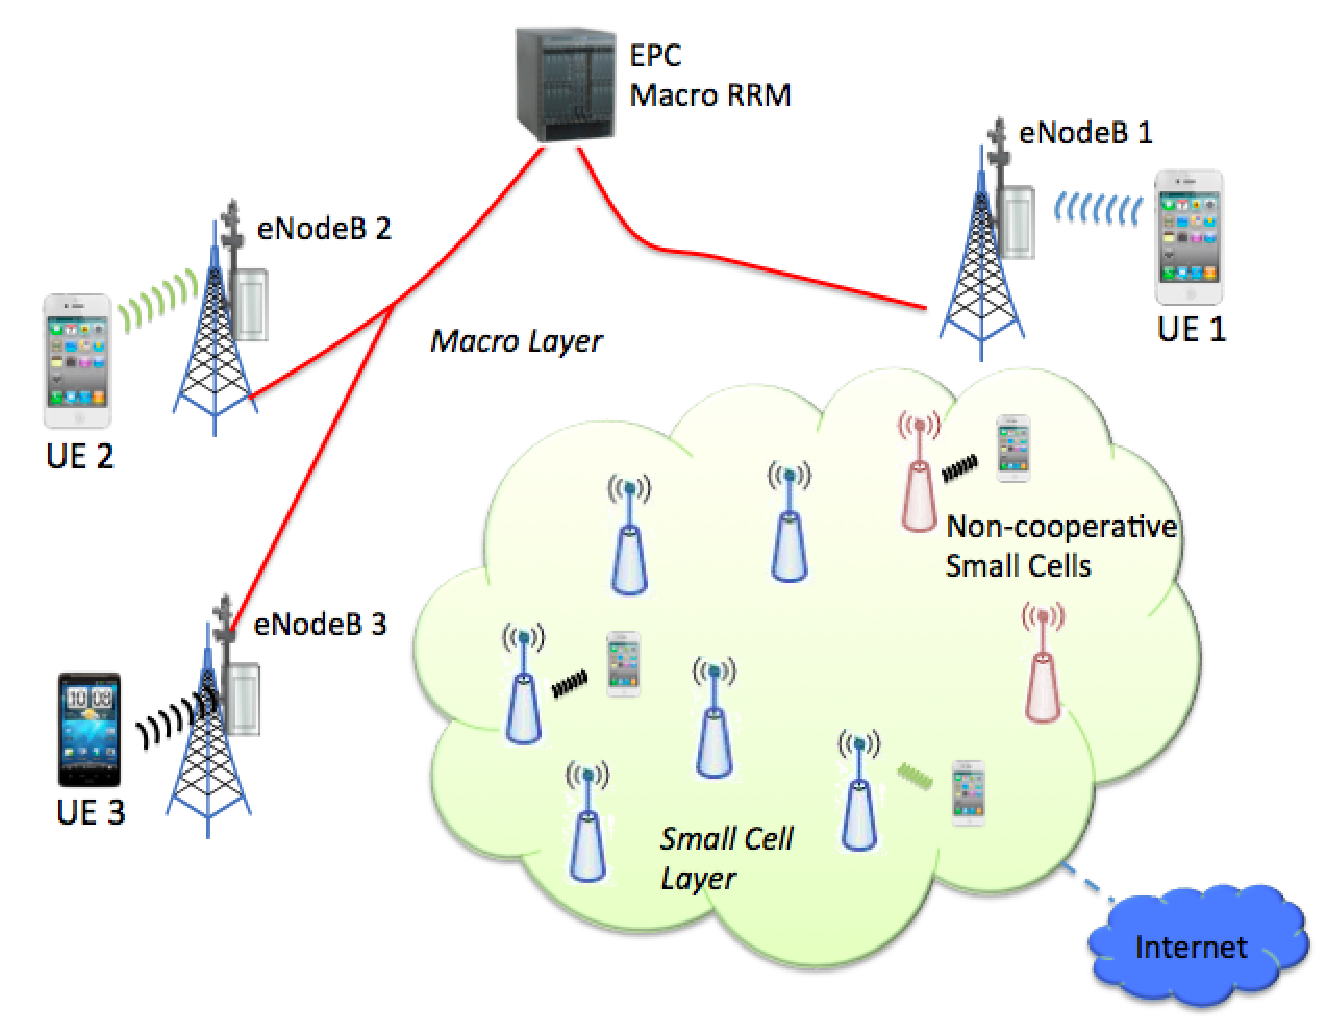
\includegraphics[width=8cm]{gcimages/architecture}
    \caption{Архитектура сети: макро уровень и уровень малых сот (кооперативные и некооперативные)}
    \label{fig:architecture}
\end{figure}

Рис.~\ref{fig:architecture} иллюстрирует типичный сценарий развертывания гетерогенных сетей~\cite{6824744}, которые обычно встречаются на практике. Они состоят из следующих элементов:

\begin{itemize}
\item[$\cdot$] Базовые макро станции (или eNodeB), которые используются для обеспечения основного покрытия сотовой сети. Базовые станции обычно конфигурируются по заранее подготовленным схемам, полученной на предварительном этапе радио-планирования. Качество покрытия базовых макро станций обычно ухудшается на границах соты и в помещениях из-за потерь сигнала и многолучевого замирания. 
\item[$\cdot$] Малые соты (HeNBs) - базовые станции малой дальности, которые в основном развернуты внутри помещений. Малые соты преимущественно развертываются без предварительного согласования и эксплуатируются без контроля со стороны оператора.
\item[$\cdot$] Некооперирующие соты - отдельный класс сетевых элементов, статически настроенные сотовым оператором или по какой-то причине действующие в рамках иных наборов правил, нежели рассматриваемые малые соты. В данной работе эти агенты (наряду с другими источниками помех) образуют ''поведение макросреды''.
\item[$\cdot$] Абонентское оборудование (UEs) - здесь мы не делаем различий между пользователями макросот и малых сот. Мы предполагаем, что пользователя всегда обслуживают базовая станция с самым сильным сигналом (что в большинстве случаев является верным предположением на практике)
\item[$\cdot$] Транспортная инфраструктура: базовые макро станции подключаются к пакетному ядру оператора (ЕРС) через выделенную линию, тогда как малые соты соединены через интернет. Отстутсвие прямой связи между ними делает распределенное алгоритмы управления более практичным для таких систем.
\end{itemize}

\subsection{Системные требования}
В этой главе мы предъявляем следующие требования:
\begin{enumerate}
\item алгоритм должен адаптироваться к различным схемам развертывания, условиям макросреды и типам трафика~\cite{TS36.300}.
\item управление системой должно происходить без вмешательства или предварительной конфигурации (требование самоорганизации)~\cite{TS36.902}.
\item отсутствие связи с посторонними агентами, чтобы избежать проблем с качеством транспортной сети и несовместимостью с проприетарными интерфейсами.
\item скорость сходимости алгоритма должна быть сопоставима с типичной скоростью изменений в системе.
\end{enumerate}

\section{Исследование структуры целевой функции}

\subsection{Модель системы}
Мы рассматриваем систему осуществляющую передачу пользовательских данных в нисходящем канале с использованием технологии мультиплексирования с ортогональным частотным разделением каналов (OFDMA)~\cite{4534773}. Система состоит из $I$ примыкающих друг к другу базовых станций и $K$ активных пользователей (абонентских устройств). Пусть $\mathcal{I} = \{1, 2, ..., I\}$ обозначает множество базовых станций, и $\mathcal{K} = \{1, 2, ..., K\}$. Дополнительно обозначим количество пользователей, обслуживаемых базовой станцией $i$ как $K(i)$. Таким образом, $K = \sum_{i=1}^L{K(i)}$.

Множество ресурсных блоков, доступных каждой базовой станции обозначим как $\mathcal{N} = \{1,2,...,N\}$. В технологии OFDMA доступный радиоспектр разделяется на несколько каналов, где каждый из каналов состоит из последовательных ортогональных OFDM-поднесущих. Ресурсный блок (РБ) представляет собой минимальную единицу, доступную для планирования передачи данных пользователям. Он состоит из 12 последовательных поднесущих в частотной области и 7 OFDM-символов с циклическим преффиксом во временной области (6 символов для расширенного преффикса).~\cite{tichv} Ресурсы выделяются и распределяются между пользователями базовой станции каждую миллисекунду (TTI = 1мс, Transmit Time Interval).

Когда при выделении ресурсов используется простая Reuse-1 модель,  каждому ресурсному блоку сопоставляется одинаковая мощность передачи $\frac{P_{max}}{N}$,  где $P_{max}$ есть максимальная мощность передачи базовой станции в  нисходящем канале. Соотношение сигнал/шум для пользователя $k$,  подключенного к базовой станции $I$ и обслуживаемого в ресурсном блоке $n$ задается следующим выражением~(\ref{eq:sinr}):

\begin{equation}
    \label{eq:sinr}
    \sigma_{k,i,n} = \frac{\pi_{i,n} G_{k,i,n}}{N_0 + \sum_{i'\neq i}{\pi_{i',n} G_{k,i',n}}}
\end{equation}
, где $\pi_{i,n}$ - мощность передачи базовой станции $i$ в ресурсном блоке $n$, $G_{k,i,n}$ - коэффициент усиления (ослабления) канала между базовой станцией $i$ и пользовательским устройством $k$, обслуживаемым в ресурсном блоке $n$ и $N_0$ - мощность теплового шума. Индексы $i$ и $i'$ относятся к полезному и интерферирующим сигналам соответственно. Для удобства список используемых обозначений собран в таблице~\ref{tbl:notations}.


\begin{table} [htbp]
  \label{tbl:notations}
  \centering
  %\captionsetup{width=15cm}
  \caption{Используемые обозначения}\label{Ts0Sib}%
  \begin{tabular}{| p{1cm} || p{10cm} |}
  \hline
  \hline
  \centering $i$ &  Индекс базовой станции   						\\
  \centering $k$ &  Индекс пользовательского устройства     		\\
  \centering $n$ &  Индекс ресурсного блока   						\\
  \centering $\mathcal{I}$ & Множество базовых станций				\\
  \centering $\mathcal{K}$ & Множество пользовательских устройств	\\
  \centering $\mathcal{K}(i)$ & Множество пользовательских устройств, ассоциированных с базовой станцией $i$\\
  \centering $\mathcal{N}$ & Множество ресурсных блоков\\
  \centering $\rho_{k,i,n}$ & Пропускная способность пользователя $k$, обслуживаемого в ресурсном блоке $n$ базовой станции $i$\\
  \centering $\pi_{i,n}$ & Мощность передачи базовой станции $i$ в ресурсном блоке $n$\\
  \centering $G_{k,i,n}$ & Коэффициент усиления (ослабления) канала между базовой станцией $i$ и пользовательским устройством $k$\\
  \centering $N_0$ & Мощность теплового шума\\
  \centering $\theta_{k,n}$ & Процент времени, занимаемый пользователем $k$ в ресурсном блоке $n$ \\
  \centering $\sigma_{k,i,n}$ & Соотношение сигнал/шум для пользователя $k$, обслуживаемого в ресурсном блоке $n$ базовой станции $i$ \\
  \centering $P_{max}$ &  Максимальная мощность передачи базовой станции в  нисходящем канале\\
  \centering $\pi_{min}$ & Минимальная мощность передачи в ресурсном блоке \\
  \centering $\mathcal{I}'(i)$ & Множество базовых станций смежных с $i$\\
  \hline
  \hline
  \end{tabular}
\end{table}

\subsection{Постановка оптимизационной задачи}
В данном разделе ставится цель максимизировать суммарную пропускную способность сети базовых станций с обеспечением честности распределения ресурсов между пользователями за счет управления мощностью передачи в реcурсных блоков. Пиковая пропускная способность пользователя $k$, обслуживаемого в ресурсном блоке $n$ базовой станции $i$ задается следующим образом:

\begin{equation}
    \label{eq:throughput}
    \rho_{k,i,n} = \log \left(1 + \frac{\pi_{i,n} G_{k,i,n}}{N_0 + \sum_{i'\neq i}{\pi_{i',n} G_{k,i',n}}}\right)
\end{equation}

Обозначим за $\theta_{k,n}$ процент времени, занимаемый пользователем $k$ в ресурсном блоке $n$. Таким образом, средняя пропускная способность для пользователя задается следующим выражением~(\ref{eq:uthroughput}):

\begin{equation}
    \label{eq:uthroughput}
    \sum_{n \in \mathcal{N}} \theta_{k,n} \cdot \rho_{k,i,n}
\end{equation}

Задачу оптимизации для рассматриваемого сценария можно сформулировать следующим образом. Целевая функция $\eta(\pi, \theta)$ состоит из суммы логарифмов показателей пропускной способности для обслуживаемых пользователей.

\begin{equation}
\label{eq:maximize}
\eta = \sum_{i \in \mathcal{I}} \sum_{k \in \mathcal{K}(i)} \log \left(\sum_{n \in \mathcal{N}} \theta_{k,n} \cdot \log \left(1 + \frac{\pi_{i,n} G_{k,i,n}}{N_0 + \sum_{i'\neq i}{\pi_{i',n} G_{k,i',n}}}\right)\right) 
\end{equation}

Такая структура целевой функции $\sum_{k=1}^K \log(r_k)$ (см.~(\ref{eq:maximize})) традиционно используется для максимизации суммарной пропускной способности в системах с $K$ пользователями для достижения справедливости распределения ресурсов. Может быть показано, что для решения $r^* = (r_1,r_2,...,r_K), r^* \in \Lambda$ задачи максимизации справедливо  неравенство (\ref{eq:propfairness}),  совпадающее с определением \textit{пропорционально справедливого} распределения ресурсов между $K$ пользователями~\cite{ETT:ETT4460080106}.

\begin{equation}
\label{eq:propfairness}
\sum_{k=1}^K \frac{r_k - r_k^*}{r_k^*} \leq 0, \forall r \in \Lambda
\end{equation}

Задача максимизации фукционала $\eta$ дополняется следующими ограничениями: выражения~(\ref{eq:limitationsa})--(\ref{eq:limitationsc}) гарантируют, что ресурсный блок не используется повторно сразу несколькими пользователями одной базовой станции,  ограничения~(\ref{eq:limitationsd})~и~(\ref{eq:limitationse}) соответствуют физическим ограничениям на суммарную мощность передачи по всем ресурсным блокам и минимальной мощности передачи в отдельном ресурсном блоке.

\begin{subequations}
\begin{equation}
\label{eq:limitationsa}
\sum_{k \in \mathcal{K}(i)} \theta_{k,n} \leq 1, \forall n \in \mathcal{N}
\end{equation}

\begin{equation}
\label{eq:limitationsb}
\sum_{n \in \mathcal{N}} \theta_{k,n} \leq 1, \forall k \in \mathcal{K}(i) 
\end{equation}

\begin{equation}
\label{eq:limitationsc}
0 \leq \theta_{k,n} \leq 1, \forall k \in \mathcal{K}(i), \forall n \in \mathcal{N}
\end{equation}

\begin{equation}
\label{eq:limitationsd}
\sum_{n \in \mathcal{N}} \pi_{i,n} \leq P_{max}, \forall i \in \mathcal{I}
\end{equation}

\begin{equation}
\label{eq:limitationse}
\pi_{i,n} \geq \pi_{min}, \forall i \in \mathcal{I}, \forall n \in \mathcal{N}
\end{equation}
\end{subequations}

\subsection{Декомпозиция оптимизационной задачи}
Для упрощения задачу максимизации фукционала~(\ref{eq:maximize}) возможно разделить на две независимые задачи оптимизации - задачу распределения ресурсов между пользователями и задачу управления мощностью в ресурсных блоках. Воспользуемся неравенством для выпуклой функции ($f\left(\sum _{{i=1}}^{{n}}q_{i}x_{i}\right)\leq \sum _{{i=1}}^{{n}}q_{i}f(x_{i})$), чтобы получить нижнюю оценку для целевой функции $\eta$:

\begin{equation}
    \label{eq:jensen}
    \log{\sum_{n \in \mathcal{N}} \theta_{k,n} \cdot \rho_{k,i,n}} \geq \frac{\sum_{n \in \mathcal{N}} \log{\theta_{k,n} \cdot \rho_{k,i,n}}}{|\mathcal{N}|} + \log{|\mathcal{N}|}
\end{equation}

Таким образом для получения нижней оценки максимума функции $\eta(\pi, \theta)$ (см. формулу ~(\ref{eq:maximize})) предлагается производить оптимизацию функционала $\eta'$ с ограничениями ~(\ref{eq:limitationsa})--(\ref{eq:limitationse}). В такой постановке задачу оптимизации возможно разделить на две независимые задачи - задачу распределения ресурсов между пользователями и задачу управления мощностью в ресурсных блоках.

\begin{equation}
\label{eq:maximizealt}
\eta' = \sum_{i \in \mathcal{I}} \sum_{k \in \mathcal{K}(i)} \sum_{n \in \mathcal{N}} (\log(\theta_{k,n}) + \log( \rho_{k,i,n}))
\end{equation}

\section{Схема управления на основе обучения с подкреплением}
\begin{figure}
    \centering
    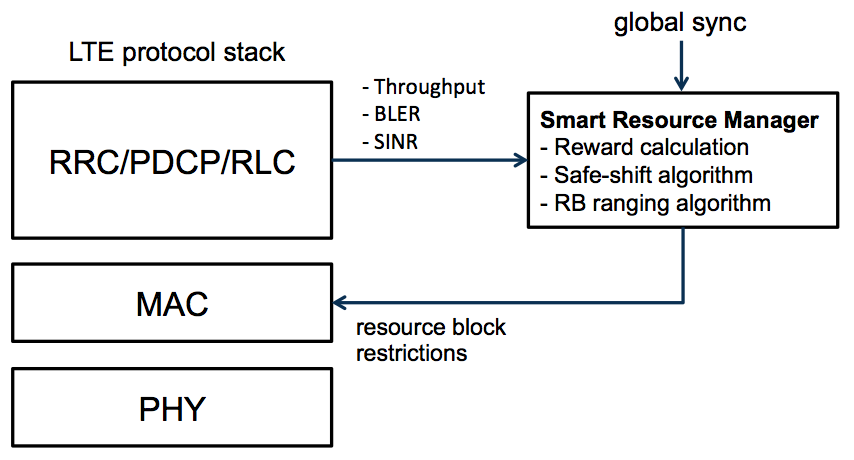
\includegraphics[width=8cm]{gcimages/algo_arch}
    \caption{Структура алгоритма и место в стеке протоколов LTE: PHY - физический уровень, MAC - уровень управления доступом к среде, RRC/PDCP/RLC - верхние уровни стека LTE}
    \label{fig:algo_arch}
\end{figure}

На Рис.~\ref{fig:algo_arch} представлена упрощенная структура алгоритма в стеке протоколов сети LTE. Можно заметить, что входящие или исходящие каналы управления не используются. Таким образом предлагаемое решение не налагает каких-либо требований на качество канала между базовыми станциями и выполняется локально на каждой малой соте.
Общий принцип алгоритма заключается в следующем. Основываясь на статистике производительности слоя L2~\cite{TS36.300} (например, BLER, спектральная эффективность) каждая малая сота локально принимает решение об использовании ресурсных блоков на последующем периоде времени. Единственный внешний входящий канал управления - глобальный источник точного времени. Он используется для выполнения синхронных операций (безопасный сдвиг) в пределах группы малых сот. После принятия решения о распределении ресурсов в каждой соте, выбранные ресурсные блоки  распределяются между пользователями базовой станции на уровне доступа к среде.

\subsection{Схема распределения радиоресурсов}
В этой части мы рассмотриваем разнородные сети LTE состоящие из множества малых сот, сосуществующих с окружающими базовыми макро станциями. Базовые макро станции и малые соты работают в одном частотном диапазоне, чтобы увеличить повторное использование пространственной частоты.

Для координации интерференции между соседними сотами каждая малая сота автономно принимает решения о распределении частот. Весь доступный частотный диапазон разбивается на ряд поддиапазонов $b_{j}$, где $j=1, .., N$ и $N$ - общее количество поддиапазонов. Распределение ресурсов внутри каждой базовой станции осуществляется планировщиком с алгоритмом пропорционального справедливого разделения (Proportional fair).

В момент времени $t$ автономный агент должен решить, какой поддиапазон $b(t+1)$ из имеющегося спектра доступен для использования на следующем временном промежутке $t+1$. Мы предлагаем схему обучения, состоящую из двух уровней (см. Рис.~\ref{fig:algo_arch}):

\begin{itemize}
\item[$\cdot$] параллельное обучение с подкреплением~\cite{4445757}, с $N\times N$ матрицей перехода $T(t)$. Она определяет вероятность перехода агента из поддиапазона $i$ в поддиапазон $j$ в момент времени $t$. Элементы матрицы периодически обновляются полученными наградами $RW_{ij}(t) = e^{(C_i(t-1) - C_j(t))}$, где $C_j(t)$ - достигаемая пропускная способность или количество пользователей с удовлетворенными требованиями к качеству обслуживания в момент времени $t$ при использовании поддиапазона $j$.
\item[$\cdot$] исследование макросреды (см. разд.~\ref{sec:safe_shift}), верхний уровень алгоритма с исследованием макросреды без вмешательства, где обучаемые агенты синхронно выполняют согласованную смену схемы использования ресурсов (безопасный сдвиг). $RW_{ij}(t_{sh})$ рассчитывается точно так же, как $RW_{ij}(t)$, но во время этапа безопасного сдвига. Этот шаг отвечает за обеспечение сосуществования с невзаимодействующими агентами и исследования макросреды.
\end{itemize}

Матрица перехода $T$ определяет вероятность перехода из поддиапазона $i$ к поддиапазону $j$. Значения $T_{ij}(t)$ и $T_{ij}(t_{sh})$ обновляются на каждой итерации (каждую 1 мс) на основе функции вознаграждения как описано в~(\ref{eq:tm_update}).
\begin{equation}
    \label{eq:tm_update}
    T_{ij}(t) = (1-\alpha-\beta)T_{ij}(t-1) + \alpha RW_{ij}(t) + \beta RW_{ij}(t_{sh})
\end{equation}
\begin{equation}
    \label{eq:tm_update_c}
    RW_{ij}(t) = e^{(C_i(t-1) - C_j(t))}
\end{equation}
где:

\begin{itemize}
\item[$\cdot$]$ \alpha$ - коэффициент обучения, определяющий скорость сходимости алгоритма и соотношение этапов исследования и эксплуатации. Оптимальное значение для этого параметра подбирается экспериментально в ходе симуляций.
\item[$\cdot$] $\beta$ - коэффициент обучения ($\beta < \alpha$) для макросреды, определяющий скорость сходимости алгоритма верхнего уровня.
\end{itemize} 

В то время как соты не имеют одинаковых знаний об уровне занятости/интерференции каждого поддиапазона, матрица перехода $T$ обновляется независимо для каждой соты. В определенной степени, это может привести к уменьшению скорости сходимости алгоритма. Моделирование показывает, что этим поведением можно эффективно управлять с помощью тонкой настройки коэффициентов обучения. В следующем разделе предложен дополнительный метод для повышения скорости сходимости алгоритма.

\subsection{Исследование макросреды: алгоритм безопасного сдвига}
\label{sec:safe_shift}
Любой агент в каждый момент времени наблюдает ответ окружающей среды $\gamma = \gamma^{CL} + \gamma^{ML}$, который состоит из двух частей: $\gamma^{CL}$ - компонент, определяемый поведением соседних агентов, а $\gamma^{ML}$ - независимый компонент, определяемый слоем макросреды.
Рисунок~\ref{fig:channel_exploration_blocked} иллюстрирует простой случай так называемой блокировки канала, где этап исследования окружающей среды $\gamma^{ML}$ агентом №2 заблокирован компонентой $\gamma^{CL}$, обусловленной выбором диапазона агента №1. Аналогичным образом на практике подавляющее большинство попыток разведки будут заблокированы ответом канала $\gamma_b^{CL}$ соседей. 

\begin{figure}
    \centering
    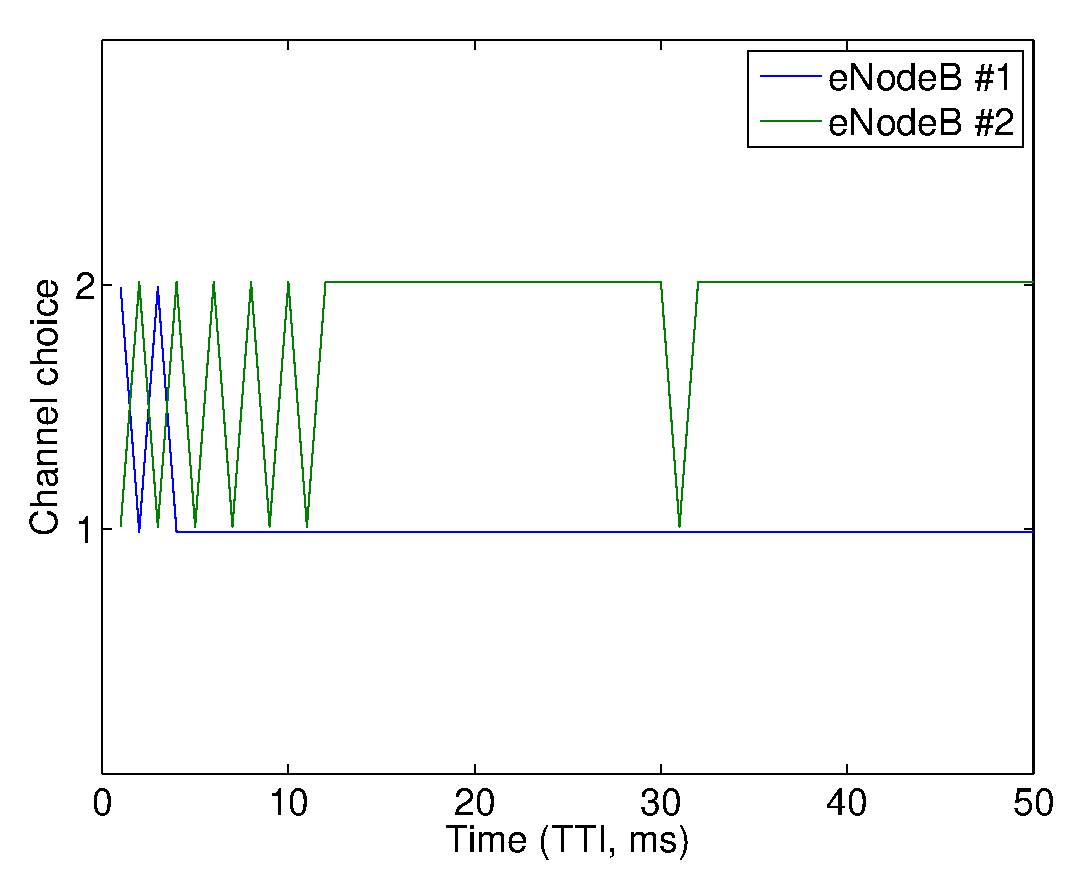
\includegraphics[width=8cm]{gcimages/channel_exploration_blocked}
    \caption{Пример эффекта блокировки канала. Оба частотных диапазона заблокированы.}
    \label{fig:channel_exploration_blocked}
\end{figure}

Чтобы побороть описанный эффект мы заставляем каждого агента изучать ответ макросреды $\gamma_b^{ML}$ в пределах каждого параллельного этапа обучения $t$ - процедуры безопасного сдвига. В рамках этой процедуры каждый агент последовательно изучает поддиапазоны в следующем порядке: ${(b_{t+1}+i)~mod~N}, i=1..N$. Очевидно, что это изменение не повлияет на компонент ответа $\gamma^{CL}$, так как агенты на пересекающихся поддиапазонах в момент времени $t$ по-прежнему используют те же поддиапазоны в момент времени ${t+1}$. В то же время компонент $\gamma^{ML}$ базового ответа окружающей среды изменяется.

Изучая отличия ответов окружающей среды $\gamma_b$, мы можем скорректировать оценки величин $\gamma_b^{ML}$ и $\gamma_b^{CL}$ для каждого агента в отдельности. Чтобы сохранить свойство локальности алгоритма, мы предлагаем управлять моментом запуска процедуры безопасного сдвига для каждого агента при помощи источника глобального времени. Значения функции вознаграждения при процедуре безопасного сдвига учитываются в соответствующей статистике для поддиапазонов в качестве отдельного компонента (см. формулу~\ref{eq:tm_update}). В результате обновления условия $\beta RW_{ij}(t_{sh})$, обучаемые агенты должны выбрать поддиапазоны с лучшим ответом макросреды.

Следующий эксперимент иллюстрирует простой пример процедуры безопасного сдвига. Рассмотрим случай двух малых сот разделяющих два частотных поддиапазона, где один из поддиапазонов занят невзаимодействующим агентом (например, базовая макро станция). После схождения процесса обучения малые соты 1 и 2 используют подздиапазоны 2 и 1 соответственно, каналы блокируются для исследования. Пусть поддиапазон 1 также занимает базовая макро станция или невзаимодействующий агент. Результат влияния процедуры безопасного сдвига на общую пропускную способность сети представлен на рис.~\ref{fig:safe_shift_overal_throughput}, где сдвиги производятся в моменты времени $t_1=200$ мс и $t_2=400$ мс. Этот шаг не влияет на взаимную интерференцию между агентами, но измененяет уровень помех от макросреды. Прирост около $10\%$ достигается без необходимости возобновления параллельного обучения для обоих агентов.

\begin{figure}
    \centering
    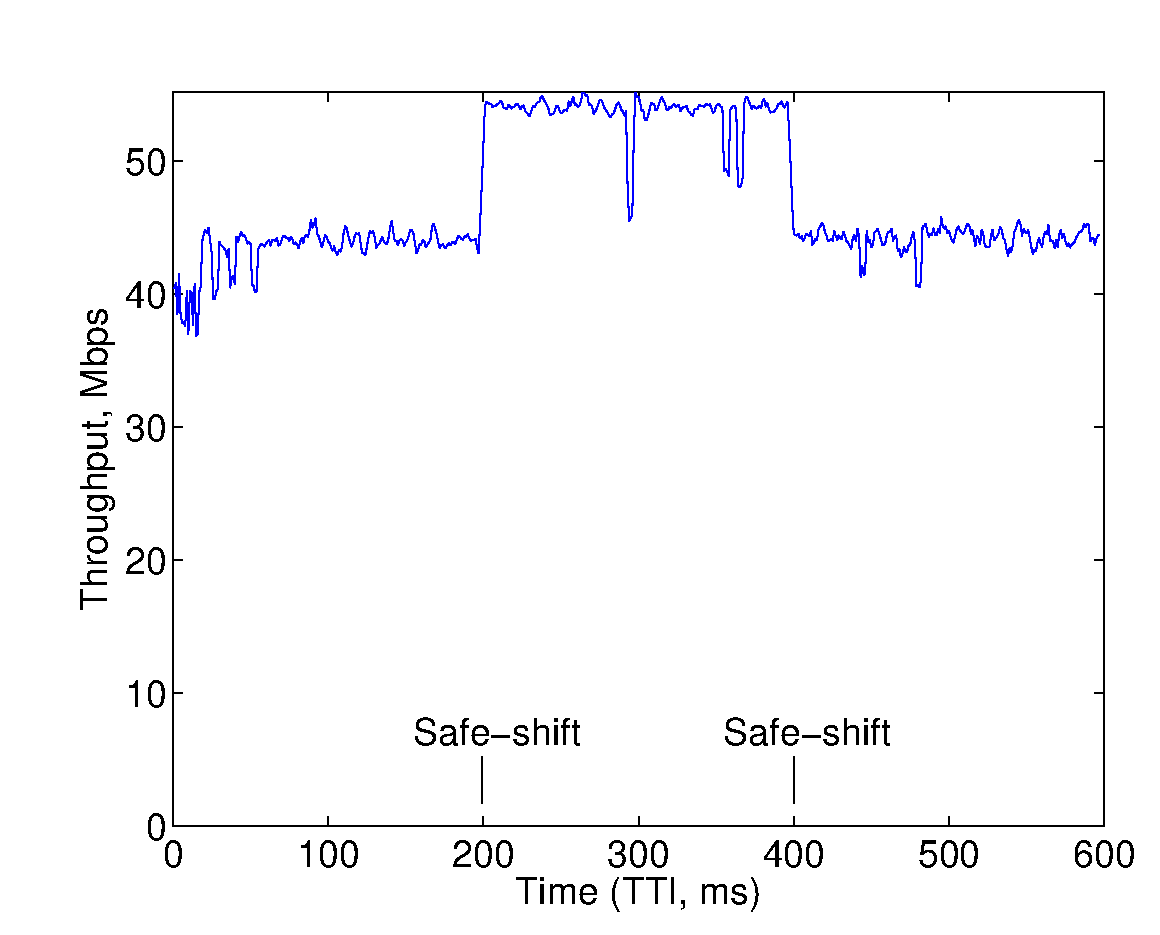
\includegraphics[width=8cm]{gcimages/overal_throughput}
    \caption{Прирост пропускной способности. Процедура безопасного сдвига инициирована в моменты времени $t_1=200$ мс и $t_2=400$ мс }
    \label{fig:safe_shift_overal_throughput}
\end{figure}

\subsection{Исследование скорости сходимости, выкалывание множества состояний}
В процессе обучения агенты постоянно изменяют свое состояние. Это в свою очередь инвалидирует стратегии других агентов, делая исходные условия, на которых они построены, устаревшими. Общий подход к этой проблеме заключается в том, чтобы считать этот эффект частью динамично изменяющейся среды. Однако, это предположение ослабляется в случае параллельного обучения множества агентов, где поведение динамической среды в большей степени определяется самими агентами.
Для того, чтобы преодолеть определяющую роль случайного исследования в структуре окружающей среды, мы предлагаем следующий способ. Идея в том, чтобы предварительно заставить агентов вести себя уникальным образом. В этом случае даже в процессе обучения посредством случайного исследования агенты могли бы получать статистически значимые наблюдения о поведении соседних агентов. Для этого мы предлагаем случайно выколоть часть $p$ $(p< 1)$ элементов матрицы перехода $TM_{ij}$ для каждого агента. Ожидается, что этот метод значительно уменьшит время сходимости процесса обучения.


\begin{figure}
    \centering
    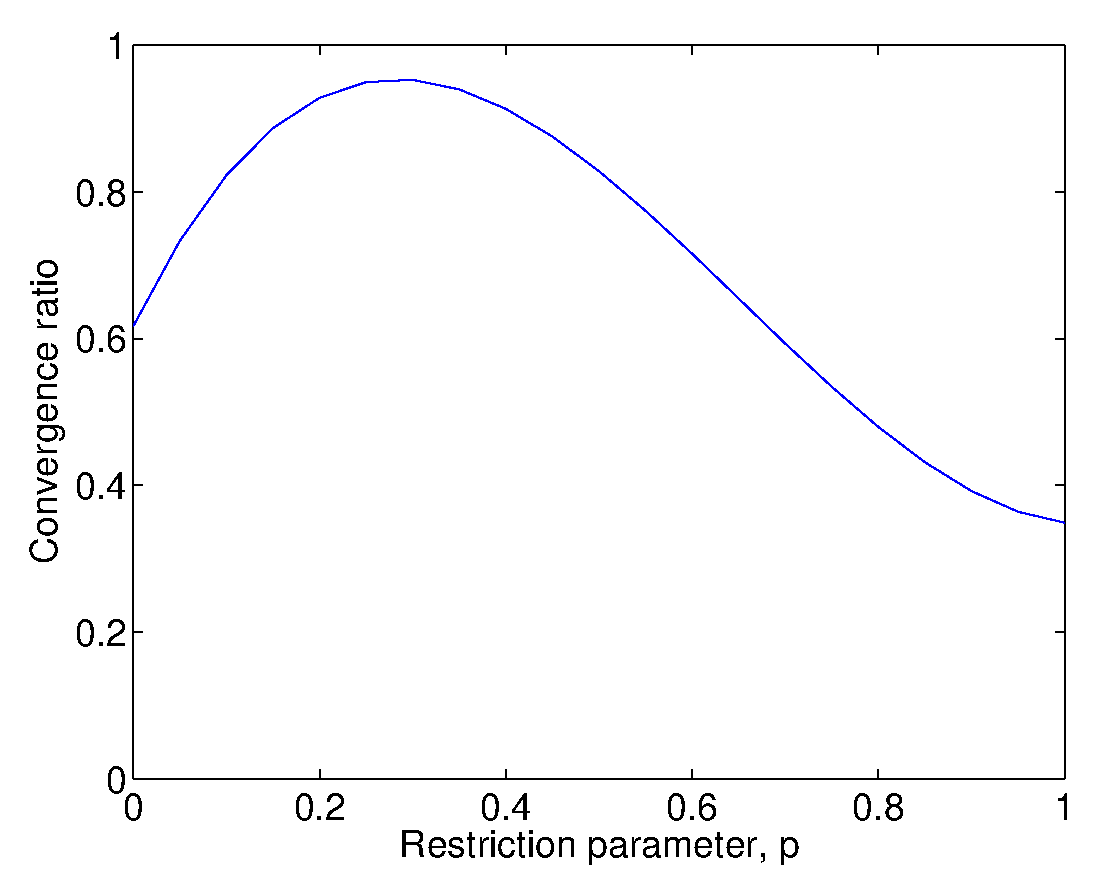
\includegraphics[width=8cm]{gcimages/restrict_p_sm}
    \caption{Средняя скорость сходимости в зависимости от параметра $p$ (тренд)}
    \label{fig:restrict_profit}
\end{figure}

На рисунке~\ref{fig:restrict_profit} проиллюстрировано поведение значения скорости сходимости в зависимости от параметра $p$ (показания усредненны для случайного набора из 500 прогонов иммитационной модели). Под скоростью сходимости понимается отношение продолжительности этапа эксплуатации к общей продолжительности работы системы. Значение $p = 0$ соответствует случаю, когда на переходные правила не накладывается никаких ограничений. Значение $p>0$ - конфигурации, когда некоторая часть переходов случайным образом запрещена для каждого агента. Видно, что для определенного значения ($p=0.3$) коэффициент сходимости увеличивается на $20\%$.

% \subsection{Channel blocking}

\section{Оценка эффективности}

Для анализа производительности, мы проводим моделирование с помощью симулятора, основанном на программном продукте Vienna LTE-A Downlink System Level Simulator (\cite{VTC2010}). Сеть состоит из 2-х уровней - группа малых сот (находящихся внутри помещения) соседствует с базовой макро станцией. Малые соты располагаются в ячейках 5х5 сетки по правилам, указанным в рекомендации консорциума 3GPP ~\cite{R4-092042}. Пользователи равномерно распределены внутри помещения. Предполагается, что каждый пользователь обслуживается базовой станцией с самым сильным сигналом. Рассматриваемые модели распространения сигнала и замирания в канале основаны на рекомендациях ~\cite{R4-092042}. Основные параметры модели, используемые по-умолчанию приведены в таблице~\ref{table:simulation_parameters}.

На рисунке~\ref{fig:fcdf3} показана интегральная функция распределения пропускной способности пользователей для множества прогонов моделирования. Предложенный алгоритм сравнивается с алгоритмом обучения, описанным в~\cite{mab}, где базовые станции принимают решения о распределении поддиапазонов с учетом занятости ресурсов каждой из окружающих сот. Видно, что предлагаемый механизм безопасного сдвига способен увеличить среднюю емкость сети на $8 - 10\%$ без негативного воздействия на честность распределения ресурсов.

\begin{table}
\centering
    \caption{Параметры моделирования}
    \begin{tabular}{|l l|} 
    \hline
    \textbf{Параметр} & \textbf{Описание} \\
    \hline
    \multicolumn{2}{|c|}{\textbf{Детали сценария}} \\
    \hline
    Основой сценарий & 5x5 Grid~\cite{R4-092042} \\
    \hline
    Выходная мощность & 23 дБм \\
    \hline
    Количество базовых станций & 7 \\
    \hline
    Количество пользователей & 28 \\
    \hline
    Планировщик & PF \\
    \hline
    Трафик & BE \\
    \hline
    Тип антенн & Всенаправленные \\
    \hline
    Ширина канала & 20 МГц \\
    \hline
    Продолжительность TTI  & 1 мс \\
    \hline
    Продолжительность симуляции & 300 TTI, 1 ч \\
    \hline
    \multicolumn{2}{|c|}{\textbf{Модель канала}} \\
    \hline
    Несущая частоты & Band 7 \\
    \hline
    Плотность мощности теплового шума  & -174 дБм/Гц \\
    \hline
    Затенение канала & Log-normal, 8 дБ \\
    \hline
    Замирание канала & Плоское замирание \\
    \hline
    \multicolumn{2}{|c|}{\textbf{Параметры алгоритма}} \\
    \hline
    $\alpha$ & 0.1 \\
    \hline
    $\beta$ & 0.05 \\
    \hline
    Коэффициент выкалывания, $p$ & 0.3 \\
    \hline
    \end{tabular}
    \label{table:simulation_parameters}
\end{table}

Эффективность предложенного алгоритма сравненивается с традиционной статической схемой разбиения полосы частот (см., например, \cite{4907410}): 

\textbf{Алгоритм Reuse 1}: каждая базовая станция использует всю доступную полосу пропускания (20 МГц, см. таблицу~\ref{table:simulation_parameters}). Затем ресурсы распределяются между пользователями с помощью пропорционального справедливого планировщика.

\textbf{Алгоритм Reuse 3}: каждой базовой станции выделяется треть всего доступного диапазона. Поддиапазонное распределение настроено так, что соседние базовые станции не используют перекрывающиеся поддиапазоны.

\begin{figure}
    \centering
    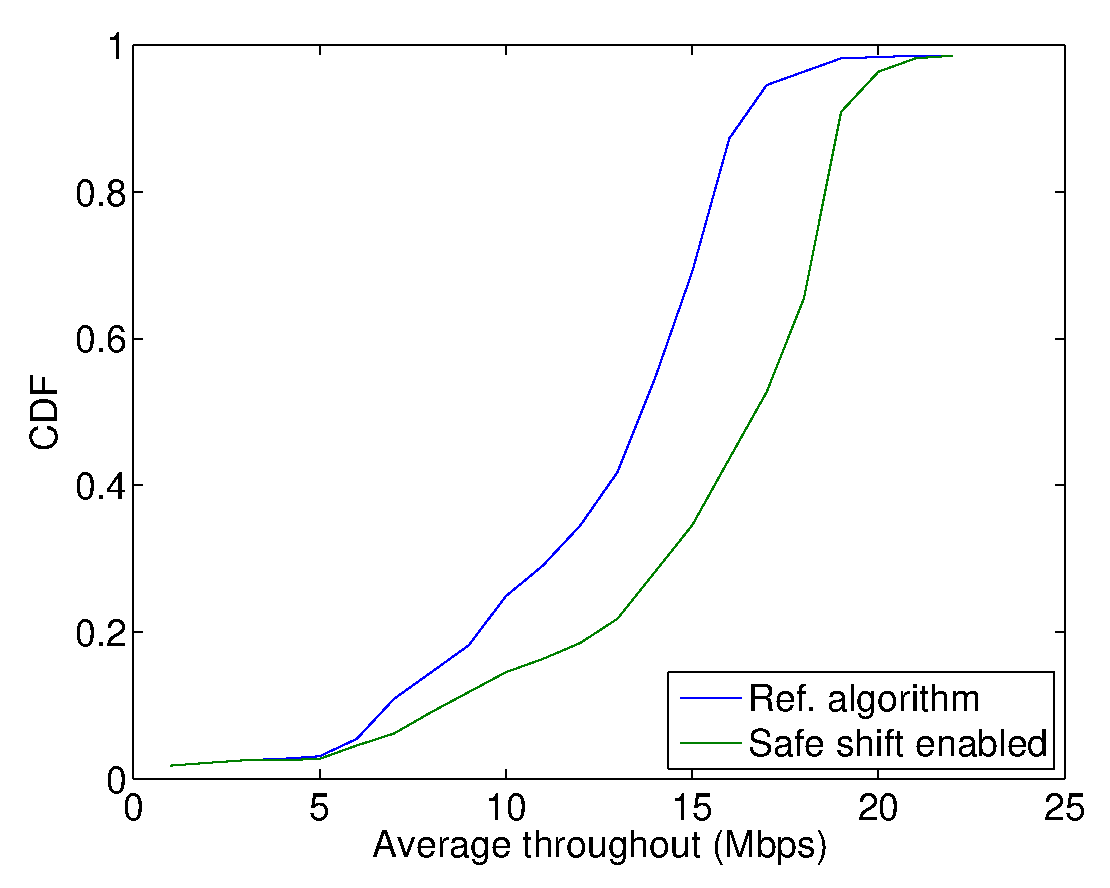
\includegraphics[width=8cm]{gcimages/fcdf3}
    \caption{Функция распределения пропускной способности для пользователей. Алгоритм безопасного сдвига}
    \label{fig:fcdf3}
\end{figure}

На рисунке ~\ref{fig:scdf} показана интегральная функция распределения соотношений сигнал-шум (SINR) для пользователей при использовании предлагаемого алгоритма разделения ресурсов. Значение SINR (соотношения сигнала к интерференции и шуму) рассчитывается для каждого пользователя после выделения ресурсных блоков.
\begin{equation}
    \label{eq:SINR}
    {SINR}_u(b) = \frac{P_u(b) G_u}{\sum_{i \in \eta} P_i(b) G_{u,i} + \sigma^2}
\end{equation}
где $P_u(b)$ - мощность передачи в ресурсном блоке $b$ при обслуживании пользователя $u$; $G_{u,i}$ - ослабление канала между пользователем $u$ и базовой станцией $i$; и $\eta$ - множество соседних базовых станций. Обратим внимание, что $P_i(b) = 0$, если базовая станция $i$ не обслуживает пользователей в поддиапазоне $b$.

\begin{figure}
    \centering
    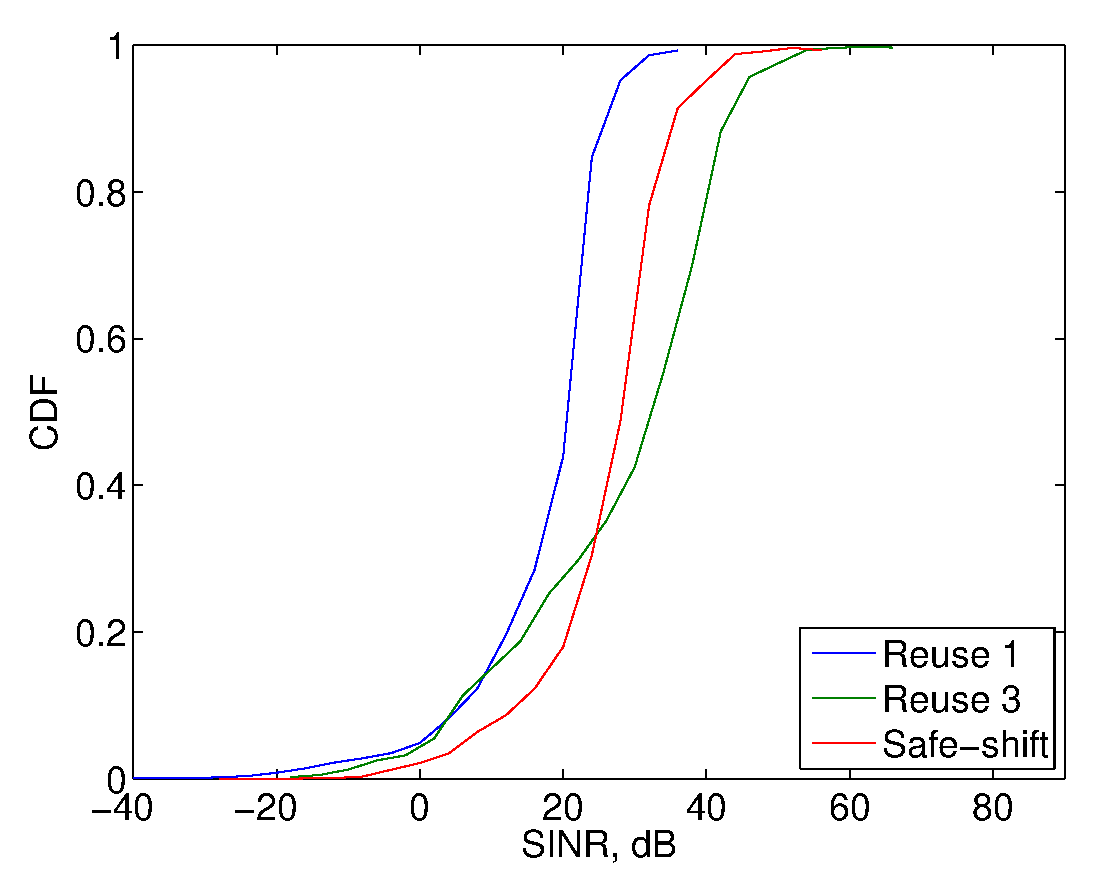
\includegraphics[width=8cm]{gcimages/scdf}
    \caption{Функция распределения соотношений сигнал-шум (SINR) для пользователей сети}
    \label{fig:scdf}
\end{figure}

Из рисунка~\ref{fig:scdf} можно заключить, что предложенный алгоритм способен самостоятельно найти оптимальную схему распределения поддиапазонов и превосходит традиционные централизованные статические схемы разделения ресурсов. Мы также отмечаем, что процедура безопасного сдвига позволяет осуществить исследование без вмешательства в ранее установленную схему распределения ресуров. Это позволяет системе сходится к более выгодной конфигурации без дополнительных затрат, связанных с автономным исследованием. Показано, что предлагаемая процедура позволяет сократить количество шагов случайного исследования среды на $20\%$, при этом оставаясь выше по эффективности на этапе эксплуатации, чем базовый алгоритм.

\section{Обсуждение}
В этой главе мы представили механизм распределения радиоресурсов для координации интерференций между соседними сотами в плотной гетерогенной сети. Он распределяет ресурсы системы на основе мультиагентного параллельного алгоритма обучения. Основной упор делается на сосуществование малых сотовых систем с невзаимодействующей макросредой. Мы также предложили прием для повышения эффективности параллельного обучения за счет снижения эффекта блокировки исследования внешней среды. Воспользовавшись так называемой процедурой безопасного сдвига, мы продемонстрировали способ повышения общей эффективности обучения и обеспечения сосуществования с окружающей средой в многоагентной среде.

Данный алгоритм предполагает гибкий механизм для контроля скорости сходимости в случае разделения радиоресурса на несколько поддиапазонов. В качестве входных данных для алгоритма, мы используем стандартные метрики 3GPP, доступные локально на любой коммерческой малой соте, что делает его легко реализуемым на практике. Вычислительная сложность алгоритма невысока всвязи с итеративным характером получения итогового решения.

Моделирование на системном уровне доказало эффективность предложенного решения в условиях реалистичных сценариев развертывания, рекомендованных консорциумом 3GPP. В нашем исследовании мы показали, что предложенный алгоритм работает в различных разнородных сценариях и превосходит эталонные алгоритмы без негативного влияния на скорость сходимости. Дальнейшие исследования направлены на развитие усовершенствованного алгоритма, способного динамически регулировать размеры поддиапазонов.
           % Глава 3
\chapter{Общие принципы применения методов машинного обучения} \label{chapt4}


Обсуждение вопросов внедрения алгоритмов ML в промышленности
http://ieeexplore.ieee.org/stamp/stamp.jsp?arnumber=7293887\&tag=1

Методология применения машинного обучения в обрабатывающей промышленности (с картинками)
http://ieeexplore.ieee.org/document/8051033/           % Глава 4
\chapter*{Заключение}						% Заголовок
\addcontentsline{toc}{chapter}{Заключение}	% Добавляем его в оглавление

%% Согласно ГОСТ Р 7.0.11-2011:
%% 5.3.3 В заключении диссертации излагают итоги выполненного исследования, рекомендации, перспективы дальнейшей разработки темы.
%% 9.2.3 В заключении автореферата диссертации излагают итоги данного исследования, рекомендации и перспективы дальнейшей разработки темы.
%% Поэтому имеет смысл сделать эту часть общей и загрузить из одного файла в автореферат и в диссертацию:

Основные результаты работы заключаются в следующем.
%% Согласно ГОСТ Р 7.0.11-2011:
%% 5.3.3 В заключении диссертации излагают итоги выполненного исследования, рекомендации, перспективы дальнейшей разработки темы.
%% 9.2.3 В заключении автореферата диссертации излагают итоги данного исследования, рекомендации и перспективы дальнейшей разработки темы.
применение машинного обучения приносит свои плоды, однако внедрение затруднено тем, что клиенты не готовы доверять автоматизированным системам такого уровня абстракций. Трактовка работы моделей на базе машинного обучения и визуализация результата является необходимой частью успешного проекта. При этом желательно, чтобы трактовка происходила в реальном времени, с привлечением экспертов рабочей группы с самого начала разработки системы.
Опыт применения методов машинного обучения к задачам управления инфраструктурой российских железных дорог на Московской железной дороге  позволяет  ожидать  положительные  практические результаты при дальнейшем развитии и тиражировании достигнутых совместной рабочей группой специалистов.
По  результатам  доклада  генерального  директора  компании  ООО «Телум»  Павла  Бойко, Ученый  совет  ОАО «РЖД»  признал  перспективным применение современных методов машинного обучения к задачам управления инфраструктурой российских железных дорог и порекомендовал продолжить развитие, разработку и внедрение си-стемы в составе более широкой совместной груп-пы, с вовлечением отраслевых институтов и университетов (в т.ч. АО«ВНИИЖТ»). Представленные наработки в области интеллектуального анализа данных также рекомендовано апробировать в других областях железнодорожного транспорта.
\begin{enumerate}
  \item \todo{На основе анализа \ldots}
  \item \todo{Численные исследования показали, что \ldots}
  \item \todo{Математическое моделирование показало \ldots}
  \item \todo{Для выполнения поставленных задач был создан \ldots}
\end{enumerate}

\todo{И какая-нибудь заключающая фраза.}

В заключение автор выражает благодарность и большую признательность научному руководителю
Кулешову~А.П. за поддержку, помощь и научное руководство.
Также автор благодарит Ботвича~Д.Д и Яроцкого~Д.А. за
помощь, обсуждение результатов и , Соколова~Е.А. за предоставление
доступа к данным и обсуждение результатов. Автор также благодарит
всех, кто сделал настоящую работу возможной.
%Филь Иванова Бойко Лаконцев Андреев Сколтех ИППИ Хоров Сколтех (за доступ к научным библиотекам)      % Заключение
\chapter*{Список сокращений и условных обозначений}             % Заголовок
\addcontentsline{toc}{chapter}{Список сокращений и условных обозначений}  % Добавляем его в оглавление
\noindent
\addtocounter{table}{-1}% Нужно откатить на единицу счетчик номеров таблиц, так как следующая таблица сделана для удобства представления информации по ГОСТ
%\begin{longtabu} to \dimexpr \textwidth-5\tabcolsep {r X}
\begin{longtabu} to \textwidth {r X}
\textbf {АРМ} & Автоматизированное рабочее место\\
\textbf {АПК-ДК} & Аппаратно-програмный комплекс диспетчерского контроля \\
\textbf {ЦП} & Управление пути Центральной Дирекции Инфрастуктуры (ЦДИ)\\
\textbf {ЦШ} & Управление Автоматики и телемеханики ЦДИ\\
\textbf {ЦУСИ} & Центр управления содержанием инфраструктуры Центральной дирекции инфраструктуры - филиала ОАО "РЖД" \\
\textbf {ЦКИ} & Департамент информатизации \\
\textbf {ПКБ И} & Проектно-конструкторское бюро инфраструктуры \\
\textbf {МЦК} & Московское центральное кольцо \\
\textbf {СЦБ} & Cигнализация, централизация, блокировка \\
\textbf {ЖАТ}   & Устройства железнодорожной автоматики и телемеханики \\
\textbf {ШНС} & Cтарший электромеханик СЦБ или связи \\
\textbf {ШЧД} & Диспетчер дистанции или дежурный инженер дистанции \\
\textbf {Ш} & Cлужба сигнализации и связи \\
\textbf {ШЧ} & Дистанция сигнализации, централизации и блокировки \\
\textbf {ПЧ} & Дистанция пути, начальник дистанции пути \\
\textbf {ЭЧ} & Дистанция электроснабжения, начальник дистанции электроснабжения \\
\textbf {ТЧ} & Тяговая часть (локомотивное депо); начальник депо \\
\textbf{AMC}	&	Adaptive Modulation and Coding \\
\textbf{CQI}	&	Channel Quality Indicator \\
\textbf{DCE}	&	Direct Code Execution \\
\textbf{DCI}	&	Downlink Control Information \\
\textbf{DRX}	&	Discontinuous transmission/reception \\
\textbf{ENB}	&	Evolved Node B, базовая станция LTE \\
\textbf{EPC}	&	Evolved Packet Core, сеть оператора LTE \\
\textbf{E-UTRAN}	&	Evolved Universal Terrestrial Radio Access Network,  сеть радиодоступа LTE \\
\textbf{FDPS}	&	Frequency Domain Packet Scheduling \\
\textbf{GBR}	&	Guaranteed Bit Rate \\
\textbf{HARQ}	&	Hybrid Automatic Retry reQuest \\
\textbf{hENB}	&	Home ENB, малая базовая станция LTE \\
\textbf{IR}	&	Incremental Redundancy \\
\textbf{LTE}	&	Long Term Evolution \\
\textbf{MAC}	&	Medium Access Control \\
\textbf{MCS}	&	Modulation and Coding Scheme \\
\textbf{MME}	&	Mobility Management Entity \\
\textbf{OFDM}	&	Orthogonal Frequency Division Multiplexing \\
\textbf{PCFICH}	&	Physical Control Format Indicator Channel \\
\textbf{PCI}	&	Physical Cell Identity \\
\textbf{PDCCH}	&	Physical Downlink Control Channel \\
\textbf{PDCP}	&	Packet Data Convergence Protocol \\
\textbf{PDN}	&	Packet Data Network \\
\textbf{PDSCH}	&	Physical Downlink Shared Channel \\
\textbf{PGW}	&	Packet Gateway \\
\textbf{PoP}	&	Point of Presence, точка подключения к сети оператора \\
\textbf{PSS}	&	Primary Synchronization Signal \\
\textbf{QoS}	&	Quality of Service \\
\textbf{RB}	&	Resource Block \\
\textbf{RLC}	&	Radio Link Control \\
\textbf{RRC}	&	Radio Resource Control \\
\textbf{RRM}	&	Radio Resource Management, управление ресурсами радиоканала \\
\textbf{RS}	&	Reference Signal \\
\textbf{RSRP}	&	Reference Signal Received Power \\
\textbf{RSRQ}	&	Reference Signal Received Quality \\
\textbf{RSSI}	&	Received Power Strength Indicator \\
\textbf{SaaS}	&	Software as a Service \\
\textbf{SC-FDMA}	&	Single Carrier Frequency Division Multiplexing \\
\textbf{SGW}	&	Service Gateway \\
\textbf{SINR}	&	Signal to Interference plus Noise Ratio \\
\textbf{SRS}	&	Sounding Reference Signal \\
\textbf{TCP}	&	Transmission Control Protocol \\
\textbf{TTI}	&	Transmission Time Interval \\
\textbf{UDP}	&	User Datagram Protocol \\
\textbf{UE}	&	User Equipment, абонентское устройство \\


\end{longtabu}
        % Список сокращений и условных обозначений
\include{Dissertation/dictionary}      % Словарь терминов
\include{Dissertation/references}      % Список литературы
\include{Dissertation/lists}           % Списки таблиц и изображений (иллюстративный материал)
\input{Dissertation/appendixsetup}   % Предварительные настройки для правильного подключения Приложений
\chapter{Примеры вставки листингов программного кода} \label{AppendixA}

Для крупных листингов есть два способа. Первый красивый, но в нём могут быть проблемы с поддержкой кириллицы (у вас может встречаться в комментариях и
печатаемых сообщениях), он представлен на листинге~\ref{list:hwbeauty}.
\begin{ListingEnv}[!h]% настройки floating аналогичны окружению figure
%    \captionsetup{format=tablenocaption}% должен стоять до самого caption
    \caption{Программа “Hello, world” на \protect\cpp}
    % далее метка для ссылки:
    \label{list:hwbeauty}
    % окружение учитывает пробелы и табуляции и применяет их в сответсвии с настройками
    \begin{lstlisting}[language={[ISO]C++}]
	#include <iostream>
	using namespace std;

	int main() //кириллица в комментариях при xelatex и lualatex имеет проблемы с пробелами
	{
		cout << "Hello, world" << endl; //latin letters in commentaries
		system("pause");
		return 0;
	}
    \end{lstlisting}
\end{ListingEnv}%
Второй не такой красивый, но без ограничений (см.~листинг~\ref{list:hwplain}).
\begin{ListingEnv}[!h]
    \caption{Программа “Hello, world” без подсветки}
    \label{list:hwplain}
    \begin{Verb}
        
        #include <iostream>
        using namespace std;
        
        int main() //кириллица в комментариях
        {
            cout << "Привет, мир" << endl;
        }
    \end{Verb}
\end{ListingEnv}

Можно использовать первый для вставки небольших фрагментов
внутри текста, а второй для вставки полного
кода в приложении, если таковое имеется.

Если нужно вставить совсем короткий пример кода (одна или две строки), то выделение  линейками и нумерация может смотреться чересчур громоздко. В таких случаях можно использовать окружения \texttt{lstlisting} или \texttt{Verb} без \texttt{ListingEnv}. Приведём такой пример с указанием языка программирования, отличного от заданного по умолчанию:
\begin{lstlisting}[language=Haskell]
fibs = 0 : 1 : zipWith (+) fibs (tail fibs)
\end{lstlisting}
Такое решение~--- со вставкой нумерованных листингов покрупнее
и вставок без выделения для маленьких фрагментов~--- выбрано,
например, в книге Эндрю Таненбаума и Тодда Остина по архитектуре
%компьютера~\autocite{TanAus2013} (см.~рис.~\ref{fig:tan-aus}).

Наконец, для оформления идентификаторов внутри строк
(функция \lstinline{main} и тому подобное) используется
\texttt{lstinline} или, самое простое, моноширинный текст
(\texttt{\textbackslash texttt}).


Пример~\ref{list:internal3}, иллюстрирующий подключение переопределённого языка. Может быть полезным, если подсветка кода работает криво. Без дополнительного окружения, с подписью и ссылкой, реализованной встроенным средством.
\begin{lstlisting}[language={Renhanced},caption={Пример листинга c подписью собственными средствами},label={list:internal3}]
## Caching the Inverse of a Matrix

## Matrix inversion is usually a costly computation and there may be some
## benefit to caching the inverse of a matrix rather than compute it repeatedly
## This is a pair of functions that cache the inverse of a matrix.

## makeCacheMatrix creates a special "matrix" object that can cache its inverse

makeCacheMatrix <- function(x = matrix()) {#кириллица в комментариях при xelatex и lualatex имеет проблемы с пробелами
    i <- NULL
    set <- function(y) {
        x <<- y
        i <<- NULL
    }
    get <- function() x
    setSolved <- function(solve) i <<- solve
    getSolved <- function() i
    list(set = set, get = get,
    setSolved = setSolved,
    getSolved = getSolved)
    
}


## cacheSolve computes the inverse of the special "matrix" returned by
## makeCacheMatrix above. If the inverse has already been calculated (and the
## matrix has not changed), then the cachesolve should retrieve the inverse from
## the cache.

cacheSolve <- function(x, ...) {
    ## Return a matrix that is the inverse of 'x'
    i <- x$getSolved()
    if(!is.null(i)) {
        message("getting cached data")
        return(i)
    }
    data <- x$get()
    i <- solve(data, ...)
    x$setSolved(i)
    i  
}
\end{lstlisting} %$ %Комментарий для корректной подсветки синтаксиса
                 %вне листинга

Листинг~\ref{list:external1} подгружается из внешнего файла. Приходится загружать без окружения дополнительного. Иначе по страницам не переносится.
    \lstinputlisting[lastline=78,language={R},caption={Листинг из внешнего файла},label={list:external1}]{listings/run_analysis.R}






\chapter{Очень длинное название второго приложения, в котором продемонстрирована работа с длинными таблицами} \label{AppendixB}

 \section{Подраздел приложения}\label{AppendixB1}
Вот размещается длинная таблица:
\fontsize{10pt}{10pt}\selectfont
\begin{longtable*}[c]{|l|c|l|l|} %longtable* появляется из пакета caption и даёт ненумерованную таблицу
% \caption{Описание входных файлов модели}\label{Namelists} 
%\\ 
 \hline
 %\multicolumn{4}{|c|}{\textbf{Файл puma\_namelist}}        \\ \hline
 Параметр & Умолч. & Тип & Описание               \\ \hline
                                              \endfirsthead   \hline
 \multicolumn{4}{|c|}{\small\slshape (продолжение)}        \\ \hline
 Параметр & Умолч. & Тип & Описание               \\ \hline
                                              \endhead        \hline
% \multicolumn{4}{|c|}{\small\slshape (окончание)}        \\ \hline
% Параметр & Умолч. & Тип & Описание               \\ \hline
%                                             \endlasthead        \hline
 \multicolumn{4}{|r|}{\small\slshape продолжение следует}  \\ \hline
                                              \endfoot        \hline
                                              \endlastfoot
 \multicolumn{4}{|l|}{\&INP}        \\ \hline 
 kick & 1 & int & 0: инициализация без шума ($p_s = const$) \\
      &   &     & 1: генерация белого шума                  \\
      &   &     & 2: генерация белого шума симметрично относительно \\
  & & & экватора    \\
 mars & 0 & int & 1: инициализация модели для планеты Марс     \\
 kick & 1 & int & 0: инициализация без шума ($p_s = const$) \\
      &   &     & 1: генерация белого шума                  \\
      &   &     & 2: генерация белого шума симметрично относительно \\
  & & & экватора    \\
 mars & 0 & int & 1: инициализация модели для планеты Марс     \\
kick & 1 & int & 0: инициализация без шума ($p_s = const$) \\
      &   &     & 1: генерация белого шума                  \\
      &   &     & 2: генерация белого шума симметрично относительно \\
  & & & экватора    \\
 mars & 0 & int & 1: инициализация модели для планеты Марс     \\
kick & 1 & int & 0: инициализация без шума ($p_s = const$) \\
      &   &     & 1: генерация белого шума                  \\
      &   &     & 2: генерация белого шума симметрично относительно \\
  & & & экватора    \\
 mars & 0 & int & 1: инициализация модели для планеты Марс     \\
kick & 1 & int & 0: инициализация без шума ($p_s = const$) \\
      &   &     & 1: генерация белого шума                  \\
      &   &     & 2: генерация белого шума симметрично относительно \\
  & & & экватора    \\
 mars & 0 & int & 1: инициализация модели для планеты Марс     \\
kick & 1 & int & 0: инициализация без шума ($p_s = const$) \\
      &   &     & 1: генерация белого шума                  \\
      &   &     & 2: генерация белого шума симметрично относительно \\
  & & & экватора    \\
 mars & 0 & int & 1: инициализация модели для планеты Марс     \\
kick & 1 & int & 0: инициализация без шума ($p_s = const$) \\
      &   &     & 1: генерация белого шума                  \\
      &   &     & 2: генерация белого шума симметрично относительно \\
  & & & экватора    \\
 mars & 0 & int & 1: инициализация модели для планеты Марс     \\
kick & 1 & int & 0: инициализация без шума ($p_s = const$) \\
      &   &     & 1: генерация белого шума                  \\
      &   &     & 2: генерация белого шума симметрично относительно \\
  & & & экватора    \\
 mars & 0 & int & 1: инициализация модели для планеты Марс     \\
kick & 1 & int & 0: инициализация без шума ($p_s = const$) \\
      &   &     & 1: генерация белого шума                  \\
      &   &     & 2: генерация белого шума симметрично относительно \\
  & & & экватора    \\
 mars & 0 & int & 1: инициализация модели для планеты Марс     \\
kick & 1 & int & 0: инициализация без шума ($p_s = const$) \\
      &   &     & 1: генерация белого шума                  \\
      &   &     & 2: генерация белого шума симметрично относительно \\
  & & & экватора    \\
 mars & 0 & int & 1: инициализация модели для планеты Марс     \\
kick & 1 & int & 0: инициализация без шума ($p_s = const$) \\
      &   &     & 1: генерация белого шума                  \\
      &   &     & 2: генерация белого шума симметрично относительно \\
  & & & экватора    \\
 mars & 0 & int & 1: инициализация модели для планеты Марс     \\
kick & 1 & int & 0: инициализация без шума ($p_s = const$) \\
      &   &     & 1: генерация белого шума                  \\
      &   &     & 2: генерация белого шума симметрично относительно \\
  & & & экватора    \\
 mars & 0 & int & 1: инициализация модели для планеты Марс     \\
kick & 1 & int & 0: инициализация без шума ($p_s = const$) \\
      &   &     & 1: генерация белого шума                  \\
      &   &     & 2: генерация белого шума симметрично относительно \\
  & & & экватора    \\
 mars & 0 & int & 1: инициализация модели для планеты Марс     \\
kick & 1 & int & 0: инициализация без шума ($p_s = const$) \\
      &   &     & 1: генерация белого шума                  \\
      &   &     & 2: генерация белого шума симметрично относительно \\
  & & & экватора    \\
 mars & 0 & int & 1: инициализация модели для планеты Марс     \\
kick & 1 & int & 0: инициализация без шума ($p_s = const$) \\
      &   &     & 1: генерация белого шума                  \\
      &   &     & 2: генерация белого шума симметрично относительно \\
  & & & экватора    \\
 mars & 0 & int & 1: инициализация модели для планеты Марс     \\
 \hline
  %& & & $\:$ \\ 
 \multicolumn{4}{|l|}{\&SURFPAR}        \\ \hline
kick & 1 & int & 0: инициализация без шума ($p_s = const$) \\
      &   &     & 1: генерация белого шума                  \\
      &   &     & 2: генерация белого шума симметрично относительно \\
  & & & экватора    \\
 mars & 0 & int & 1: инициализация модели для планеты Марс     \\
kick & 1 & int & 0: инициализация без шума ($p_s = const$) \\
      &   &     & 1: генерация белого шума                  \\
      &   &     & 2: генерация белого шума симметрично относительно \\
  & & & экватора    \\
 mars & 0 & int & 1: инициализация модели для планеты Марс     \\
kick & 1 & int & 0: инициализация без шума ($p_s = const$) \\
      &   &     & 1: генерация белого шума                  \\
      &   &     & 2: генерация белого шума симметрично относительно \\
  & & & экватора    \\
 mars & 0 & int & 1: инициализация модели для планеты Марс     \\
kick & 1 & int & 0: инициализация без шума ($p_s = const$) \\
      &   &     & 1: генерация белого шума                  \\
      &   &     & 2: генерация белого шума симметрично относительно \\
  & & & экватора    \\
 mars & 0 & int & 1: инициализация модели для планеты Марс     \\
kick & 1 & int & 0: инициализация без шума ($p_s = const$) \\
      &   &     & 1: генерация белого шума                  \\
      &   &     & 2: генерация белого шума симметрично относительно \\
  & & & экватора    \\
 mars & 0 & int & 1: инициализация модели для планеты Марс     \\
kick & 1 & int & 0: инициализация без шума ($p_s = const$) \\
      &   &     & 1: генерация белого шума                  \\
      &   &     & 2: генерация белого шума симметрично относительно \\
  & & & экватора    \\
 mars & 0 & int & 1: инициализация модели для планеты Марс     \\
kick & 1 & int & 0: инициализация без шума ($p_s = const$) \\
      &   &     & 1: генерация белого шума                  \\
      &   &     & 2: генерация белого шума симметрично относительно \\
  & & & экватора    \\
 mars & 0 & int & 1: инициализация модели для планеты Марс     \\
kick & 1 & int & 0: инициализация без шума ($p_s = const$) \\
      &   &     & 1: генерация белого шума                  \\
      &   &     & 2: генерация белого шума симметрично относительно \\
  & & & экватора    \\
 mars & 0 & int & 1: инициализация модели для планеты Марс     \\
kick & 1 & int & 0: инициализация без шума ($p_s = const$) \\
      &   &     & 1: генерация белого шума                  \\
      &   &     & 2: генерация белого шума симметрично относительно \\
  & & & экватора    \\
 mars & 0 & int & 1: инициализация модели для планеты Марс     \\ 
 \hline 
\end{longtable*}

\normalsize% возвращаем шрифт к нормальному
\section{Ещё один подраздел приложения} \label{AppendixB2}

Нужно больше подразделов приложения!

Пример длинной таблицы с записью продолжения по ГОСТ 2.105
\begingroup
    \centering
	\small
    \begin{longtable}[c]{|l|c|l|l|}
	\caption{Наименование таблицы средней длины}%
    \label{tbl:test5}% label всегда желательно идти после caption
    \\
    \hline
     %\multicolumn{4}{|c|}{\textbf{Файл puma\_namelist}}        \\ \hline
     Параметр & Умолч. & Тип & Описание\\ \hline
     \endfirsthead%
%     \multicolumn{4}{|c|}{\small\slshape (продолжение)}        \\ \hline
 \captionsetup{format=tablenocaption,labelformat=continued}% должен стоять до самого caption
    \caption[]{}\\
    \hline
     Параметр & Умолч. & Тип & Описание\\ \hline
      \endhead
      \hline
%     \multicolumn{4}{|r|}{\small\slshape продолжение следует}  \\
%\hline
     \endfoot
         \hline
     \endlastfoot
     \multicolumn{4}{|l|}{\&INP}        \\ \hline 
     kick & 1 & int & 0: инициализация без шума ($p_s = const$) \\
          &   &     & 1: генерация белого шума                  \\
          &   &     & 2: генерация белого шума симметрично относительно \\
      & & & экватора    \\
     mars & 0 & int & 1: инициализация модели для планеты Марс     \\
     kick & 1 & int & 0: инициализация без шума ($p_s = const$) \\
          &   &     & 1: генерация белого шума                  \\
          &   &     & 2: генерация белого шума симметрично относительно \\
      & & & экватора    \\
     mars & 0 & int & 1: инициализация модели для планеты Марс     \\
    kick & 1 & int & 0: инициализация без шума ($p_s = const$) \\
          &   &     & 1: генерация белого шума                  \\
          &   &     & 2: генерация белого шума симметрично относительно \\
      & & & экватора    \\
     mars & 0 & int & 1: инициализация модели для планеты Марс     \\
    kick & 1 & int & 0: инициализация без шума ($p_s = const$) \\
          &   &     & 1: генерация белого шума                  \\
          &   &     & 2: генерация белого шума симметрично относительно \\
      & & & экватора    \\
     mars & 0 & int & 1: инициализация модели для планеты Марс     \\
    kick & 1 & int & 0: инициализация без шума ($p_s = const$) \\
          &   &     & 1: генерация белого шума                  \\
          &   &     & 2: генерация белого шума симметрично относительно \\
      & & & экватора    \\
     mars & 0 & int & 1: инициализация модели для планеты Марс     \\
    kick & 1 & int & 0: инициализация без шума ($p_s = const$) \\
          &   &     & 1: генерация белого шума                  \\
          &   &     & 2: генерация белого шума симметрично относительно \\
      & & & экватора    \\
     mars & 0 & int & 1: инициализация модели для планеты Марс     \\
    kick & 1 & int & 0: инициализация без шума ($p_s = const$) \\
          &   &     & 1: генерация белого шума                  \\
          &   &     & 2: генерация белого шума симметрично относительно \\
      & & & экватора    \\
     mars & 0 & int & 1: инициализация модели для планеты Марс     \\
    kick & 1 & int & 0: инициализация без шума ($p_s = const$) \\
          &   &     & 1: генерация белого шума                  \\
          &   &     & 2: генерация белого шума симметрично относительно \\
      & & & экватора    \\
     mars & 0 & int & 1: инициализация модели для планеты Марс     \\
    kick & 1 & int & 0: инициализация без шума ($p_s = const$) \\
          &   &     & 1: генерация белого шума                  \\
          &   &     & 2: генерация белого шума симметрично относительно \\
      & & & экватора    \\
     mars & 0 & int & 1: инициализация модели для планеты Марс     \\
    kick & 1 & int & 0: инициализация без шума ($p_s = const$) \\
          &   &     & 1: генерация белого шума                  \\
          &   &     & 2: генерация белого шума симметрично относительно \\
      & & & экватора    \\
     mars & 0 & int & 1: инициализация модели для планеты Марс     \\
    kick & 1 & int & 0: инициализация без шума ($p_s = const$) \\
          &   &     & 1: генерация белого шума                  \\
          &   &     & 2: генерация белого шума симметрично относительно \\
      & & & экватора    \\
     mars & 0 & int & 1: инициализация модели для планеты Марс     \\
    kick & 1 & int & 0: инициализация без шума ($p_s = const$) \\
          &   &     & 1: генерация белого шума                  \\
          &   &     & 2: генерация белого шума симметрично относительно \\
      & & & экватора    \\
     mars & 0 & int & 1: инициализация модели для планеты Марс     \\
    kick & 1 & int & 0: инициализация без шума ($p_s = const$) \\
          &   &     & 1: генерация белого шума                  \\
          &   &     & 2: генерация белого шума симметрично относительно \\
      & & & экватора    \\
     mars & 0 & int & 1: инициализация модели для планеты Марс     \\
    kick & 1 & int & 0: инициализация без шума ($p_s = const$) \\
          &   &     & 1: генерация белого шума                  \\
          &   &     & 2: генерация белого шума симметрично относительно \\
      & & & экватора    \\
     mars & 0 & int & 1: инициализация модели для планеты Марс     \\
    kick & 1 & int & 0: инициализация без шума ($p_s = const$) \\
          &   &     & 1: генерация белого шума                  \\
          &   &     & 2: генерация белого шума симметрично относительно \\
      & & & экватора    \\
     mars & 0 & int & 1: инициализация модели для планеты Марс     \\
     \hline
      %& & & $\:$ \\ 
     \multicolumn{4}{|l|}{\&SURFPAR}        \\ \hline
    kick & 1 & int & 0: инициализация без шума ($p_s = const$) \\
          &   &     & 1: генерация белого шума                  \\
          &   &     & 2: генерация белого шума симметрично относительно \\
      & & & экватора    \\
     mars & 0 & int & 1: инициализация модели для планеты Марс     \\
    kick & 1 & int & 0: инициализация без шума ($p_s = const$) \\
          &   &     & 1: генерация белого шума                  \\
          &   &     & 2: генерация белого шума симметрично относительно \\
      & & & экватора    \\
     mars & 0 & int & 1: инициализация модели для планеты Марс     \\
    kick & 1 & int & 0: инициализация без шума ($p_s = const$) \\
          &   &     & 1: генерация белого шума                  \\
          &   &     & 2: генерация белого шума симметрично относительно \\
      & & & экватора    \\
     mars & 0 & int & 1: инициализация модели для планеты Марс     \\
    kick & 1 & int & 0: инициализация без шума ($p_s = const$) \\
          &   &     & 1: генерация белого шума                  \\
          &   &     & 2: генерация белого шума симметрично относительно \\
      & & & экватора    \\
     mars & 0 & int & 1: инициализация модели для планеты Марс     \\
    kick & 1 & int & 0: инициализация без шума ($p_s = const$) \\
          &   &     & 1: генерация белого шума                  \\
          &   &     & 2: генерация белого шума симметрично относительно \\
      & & & экватора    \\
     mars & 0 & int & 1: инициализация модели для планеты Марс     \\
    kick & 1 & int & 0: инициализация без шума ($p_s = const$) \\
          &   &     & 1: генерация белого шума                  \\
          &   &     & 2: генерация белого шума симметрично относительно \\
      & & & экватора    \\
     mars & 0 & int & 1: инициализация модели для планеты Марс     \\
    kick & 1 & int & 0: инициализация без шума ($p_s = const$) \\
          &   &     & 1: генерация белого шума                  \\
          &   &     & 2: генерация белого шума симметрично относительно \\
      & & & экватора    \\
     mars & 0 & int & 1: инициализация модели для планеты Марс     \\
    kick & 1 & int & 0: инициализация без шума ($p_s = const$) \\
          &   &     & 1: генерация белого шума                  \\
          &   &     & 2: генерация белого шума симметрично относительно \\
      & & & экватора    \\
     mars & 0 & int & 1: инициализация модели для планеты Марс     \\
    kick & 1 & int & 0: инициализация без шума ($p_s = const$) \\
          &   &     & 1: генерация белого шума                  \\
          &   &     & 2: генерация белого шума симметрично относительно \\
      & & & экватора    \\
     mars & 0 & int & 1: инициализация модели для планеты Марс     \\ 
%     \hline 
    \end{longtable}
\normalsize% возвращаем шрифт к нормальному
\endgroup
\section{Использование длинных таблиц с окружением \textit{longtabu}} \label{AppendixB2a}

В таблице~\ref{tbl:test-functions} более книжный вариант 
длинной таблицы, используя окружение \verb!longtabu! и разнообразные
\verb!toprule! \verb!midrule! \verb!bottomrule! из пакета
\verb!booktabs!. Чтобы визуально таблица смотрелась лучше, можно
использовать следующие параметры: в самом начале задаётся расстояние
между строчками с~помощью \verb!arraystretch!. Таблица задаётся на
всю ширину, \verb!longtabu! позволяет делить ширину колонок
пропорционально "--- тут три колонки в пропорции 1.1:1:4 "--- для каждой
колонки первый параметр в описании \verb!X[]!. Кроме того, в~таблице
убраны отступы слева и справа с помощью \verb!@{}! в
преамбуле таблицы. К первому и второму столбцу применяется
модификатор 

\verb!>{\setlength{\baselineskip}{0.7\baselineskip}}!,

\noindent который уменьшает межстрочный интервал в для текста таблиц (иначе
заголовок второго столбца значительно шире, а двухстрочное имя
сливается с окружающими). Для первой и второй колонки текст в ячейках
выравниваются по~центру как по вертикали, так и по горизонтали -
задаётся буквами \verb!m! и \verb!c! в~описании столбца \verb!X[]!. 

Так как формулы большие "--- используется окружение \verb!alignedat!,
чтобы отступ был одинаковый у всех формул "--- он сделан для всех, хотя
для большей части можно было и не использовать.  Чтобы формулы
занимали поменьше места в~каждом столбце формулы (где надо)
используется \verb!\textstyle! "--- он делает дроби меньше, у знаков
суммы и произведения "--- индексы сбоку. Иногда формулы слишком большая,
сливается со следующей, поэтому после неё ставится небольшой
дополнительный отступ \verb!\vspace*{2ex}!  Для штрафных функций "---
размер фигурных скобок задан вручную \verb!\Big\{!, т.к. не умеет
\verb!alignedat! работать с~\verb!\left! и \verb!\right! через
несколько строк/колонок.


В примечании к таблице наоборот, окружение \verb!cases! даёт слишком
большие промежутки между вариантами, чтобы их уменьшить, в конце
каждой строчки окружения использовался отрицательный дополнительный
отступ \verb!\\[-0.5em]!.



\begingroup % Ограничиваем область видимости arraystretch
\renewcommand{\arraystretch}{1.6}%% Увеличение расстояния между рядами, для улучшения восприятия.
\begin{longtabu} to \textwidth
{%
@{}>{\setlength{\baselineskip}{0.7\baselineskip}}X[1.1mc]%
>{\setlength{\baselineskip}{0.7\baselineskip}}X[mc]%
X[4]@{}%
}
        \caption{Тестовые функции для оптимизации, $D$ "---
          размерность. Для всех функций значение в точке глобального
          минимума равно нулю.\label{tbl:test-functions}}\\% label всегда желательно идти после caption 
        
        \toprule     %%% верхняя линейка
        Имя           &Стартовый диапазон параметров &Функция  \\ 
        \midrule %%% тонкий разделитель. Отделяет названия столбцов. Обязателен по ГОСТ 2.105 пункт 4.4.5 
        \endfirsthead

        \multicolumn{3}{c}{\small\slshape (продолжение)}        \\ 
        \toprule     %%% верхняя линейка
        Имя           &Стартовый диапазон параметров &Функция  \\ 
        \midrule %%% тонкий разделитель. Отделяет названия столбцов. Обязателен по ГОСТ 2.105 пункт 4.4.5 
        \endhead
        
        \multicolumn{3}{c}{\small\slshape (окончание)}        \\ 
        \toprule     %%% верхняя линейка
        Имя           &Стартовый диапазон параметров &Функция  \\ 
        \midrule %%% тонкий разделитель. Отделяет названия столбцов. Обязателен по ГОСТ 2.105 пункт 4.4.5 
        \endlasthead

        \bottomrule %%% нижняя линейка
        \multicolumn{3}{r}{\small\slshape продолжение следует}  \\ 
        \endfoot   
        \endlastfoot

        сфера         &$\left[-100,\,100\right]^D$   &
        $\begin{aligned}\textstyle f_1(x)=\sum_{i=1}^Dx_i^2\end{aligned}$                                                        \\
        Schwefel 2.22 &$\left[-10,\,10\right]^D$     &
        $\begin{aligned}\textstyle f_2(x)=\sum_{i=1}^D|x_i|+\prod_{i=1}^D|x_i|\end{aligned}$                                     \\
        Schwefel 1.2  &$\left[-100,\,100\right]^D$   &$\begin{aligned}\textstyle f_3(x)=\sum_{i=1}^D\left(\sum_{j=1}^ix_j\right)^2\end{aligned}$                               \\
        Schwefel 2.21 &$\left[-100,\,100\right]^D$   &$\begin{aligned}\textstyle f_4(x)=\max_i\!\left\{\left|x_i\right|\right\}\end{aligned}$                             \\
        Rosenbrock    &$\left[-30,\,30\right]^D$     &$\begin{aligned}\textstyle f_5(x)=\sum_{i=1}^{D-1}\left[100\!\left(x_{i+1}-x_i^2\right)^2+(x_i-1)^2\right]\end{aligned}$ \\
        ступенчатая   &$\left[-100,\,100\right]^D$   &$\begin{aligned}\textstyle f_6(x)=\sum_{i=1}^D\big\lfloor x_i+0.5\big\rfloor^2\end{aligned}$                             \\ 
зашумлённая квартическая  &$\left[-1.28,\,1.28\right]^D$ &$\begin{aligned}\textstyle f_7(x)=\sum_{i=1}^Dix_i^4+rand[0,1)\end{aligned}$\vspace*{2ex}\\
        Schwefel 2.26 &$\left[-500,\,500\right]^D$   &$\begin{aligned}f_8(x)= &\textstyle\sum_{i=1}^D-x_i\,\sin\sqrt{|x_i|}\,+ \\
                    &\vphantom{\sum}+ D\cdot
                    418.98288727243369 \end{aligned}$\\
        Rastrigin     &$\left[-5.12,\,5.12\right]^D$ &
        $\begin{aligned}\textstyle
          f_9(x)=\sum_{i=1}^D\left[x_i^2-10\,\cos(2\pi
            x_i)+10\right]\end{aligned}$\vspace*{2ex}\\
  Ackley        &$\left[-32,\,32\right]^D$     &$\begin{aligned}f_{10}(x)= &\textstyle -20\, \exp\!\left(-0.2\sqrt{\frac{1}{D}\sum_{i=1}^Dx_i^2} \right)-\\
                    &\textstyle - \exp\left(\frac{1}{D}\sum_{i=1}^D\cos(2\pi x_i)  \right)  + 20 + e \end{aligned}$ \\
        Griewank      &$\left[-600,\,600\right]^D$
        &$\begin{aligned}f_{11}(x)= &\textstyle \frac{1}{4000}
          \sum_{i=1}^{D}x_i^2 - \prod_{i=1}^D\cos\left(x_i/\sqrt{i}\right) +1     \end{aligned}$ \vspace*{3ex} \\
        штрафная 1    &$\left[-50,\,50\right]^D$     &
        $\begin{aligned}f_{12}(x)= &\textstyle \frac{\pi}{D}
          \Big\{ 10\,\sin^2(\pi y_1) +\\ &+
          \textstyle \sum_{i=1}^{D-1}(y_i-1)^2\left[1+10\,\sin^2(\pi
              y_{i+1})\right] +\\ &+(y_D-1)^2 \Big\} +\textstyle\sum_{i=1}^D u(x_i,\,10,\,100,\,4)            \end{aligned}$ \vspace*{2ex} \\
        штрафная 2    &$\left[-50,\,50\right]^D$     &
        $\begin{aligned}f_{13}(x)= &\textstyle 0.1
          \Big\{\sin^2(3\pi x_1) +\\ &+
          \textstyle \sum_{i=1}^{D-1}(x_i-1)^2\left[1+\sin^2(3 \pi
              x_{i+1})\right] + \\ &+(x_D-1)^2\left[1+\sin^2(2\pi
              x_D)\right] \Big\} +\\ &+\textstyle\sum_{i=1}^D u(x_i,\,5,\,100,\,4)            \end{aligned}$               \\
        сфера         &$\left[-100,\,100\right]^D$   &
        $\begin{aligned}\textstyle f_1(x)=\sum_{i=1}^Dx_i^2\end{aligned}$                                                        \\
        Schwefel 2.22 &$\left[-10,\,10\right]^D$     &
        $\begin{aligned}\textstyle f_2(x)=\sum_{i=1}^D|x_i|+\prod_{i=1}^D|x_i|\end{aligned}$                                     \\
        Schwefel 1.2  &$\left[-100,\,100\right]^D$   &$\begin{aligned}\textstyle f_3(x)=\sum_{i=1}^D\left(\sum_{j=1}^ix_j\right)^2\end{aligned}$                               \\
        Schwefel 2.21 &$\left[-100,\,100\right]^D$   &$\begin{aligned}\textstyle f_4(x)=\max_i\!\left\{\left|x_i\right|\right\}\end{aligned}$                             \\
        Rosenbrock    &$\left[-30,\,30\right]^D$     &$\begin{aligned}\textstyle f_5(x)=\sum_{i=1}^{D-1}\left[100\!\left(x_{i+1}-x_i^2\right)^2+(x_i-1)^2\right]\end{aligned}$ \\
        ступенчатая   &$\left[-100,\,100\right]^D$   &$\begin{aligned}\textstyle f_6(x)=\sum_{i=1}^D\big\lfloor x_i+0.5\big\rfloor^2\end{aligned}$                             \\ 
зашумлённая квартическая  &$\left[-1.28,\,1.28\right]^D$ &$\begin{aligned}\textstyle f_7(x)=\sum_{i=1}^Dix_i^4+rand[0,1)\end{aligned}$\vspace*{2ex}\\
        Schwefel 2.26 &$\left[-500,\,500\right]^D$   &$\begin{aligned}f_8(x)= &\textstyle\sum_{i=1}^D-x_i\,\sin\sqrt{|x_i|}\,+ \\
                    &\vphantom{\sum}+ D\cdot
                    418.98288727243369 \end{aligned}$\\
        Rastrigin     &$\left[-5.12,\,5.12\right]^D$ &
        $\begin{aligned}\textstyle
          f_9(x)=\sum_{i=1}^D\left[x_i^2-10\,\cos(2\pi
            x_i)+10\right]\end{aligned}$\vspace*{2ex}\\
  Ackley        &$\left[-32,\,32\right]^D$     &$\begin{aligned}f_{10}(x)= &\textstyle -20\, \exp\!\left(-0.2\sqrt{\frac{1}{D}\sum_{i=1}^Dx_i^2} \right)-\\
                    &\textstyle - \exp\left(\frac{1}{D}\sum_{i=1}^D\cos(2\pi x_i)  \right)  + 20 + e \end{aligned}$ \\
        Griewank      &$\left[-600,\,600\right]^D$
        &$\begin{aligned}f_{11}(x)= &\textstyle \frac{1}{4000}
          \sum_{i=1}^{D}x_i^2 - \prod_{i=1}^D\cos\left(x_i/\sqrt{i}\right) +1     \end{aligned}$ \vspace*{3ex} \\
        штрафная 1    &$\left[-50,\,50\right]^D$     &
        $\begin{aligned}f_{12}(x)= &\textstyle \frac{\pi}{D}
          \Big\{ 10\,\sin^2(\pi y_1) +\\ &+
          \textstyle \sum_{i=1}^{D-1}(y_i-1)^2\left[1+10\,\sin^2(\pi
              y_{i+1})\right] +\\ &+(y_D-1)^2 \Big\} +\textstyle\sum_{i=1}^D u(x_i,\,10,\,100,\,4)            \end{aligned}$ \vspace*{2ex} \\
        штрафная 2    &$\left[-50,\,50\right]^D$     &
        $\begin{aligned}f_{13}(x)= &\textstyle 0.1
          \Big\{\sin^2(3\pi x_1) +\\ &+
          \textstyle \sum_{i=1}^{D-1}(x_i-1)^2\left[1+\sin^2(3 \pi
              x_{i+1})\right] + \\ &+(x_D-1)^2\left[1+\sin^2(2\pi
              x_D)\right] \Big\} +\\ &+\textstyle\sum_{i=1}^D u(x_i,\,5,\,100,\,4)            \end{aligned}$               \\
        \midrule%%% тонкий разделитель
        \multicolumn{3}{@{}p{\textwidth}}{%
            \vspace*{-3.5ex}% этим подтягиваем повыше
            \hspace*{2.5em}% абзацный отступ - требование ГОСТ 2.105
            Примечание "---  Для функций $f_{12}$ и $f_{13}$
            используется $y_i = 1 + \frac{1}{4}(x_i+1)$ и
            $u(x_i,\,a,\,k,\,m)=\begin{cases}
k(x_i-a)^m,\quad &x_i >a\\[-0.5em]
0,\quad &-a\leq x_i \leq a\\[-0.5em]
k(-x_i-a)^m,\quad &x_i <-a
\end{cases}$  }   \\        \bottomrule %%% нижняя линейка 
\end{longtabu} 
\endgroup


\section{Форматирование внутри таблиц} \label{AppendixB3}

В таблице~\ref{tbl:other-row} пример с чересстрочным
форматированием. В \verb+userstyles.tex+  задаётся счётчик
\verb+\newcounter{rowcnt}+ который увеличивается на 1 после каждой
строчки (как указано в преамбуле таблицы). Кроме того, задаётся
условный макрос \verb+\altshape+ который выдаёт одно из
двух типов форматирования в зависимости от чётности счётчика. 

В таблице~\ref{tbl:other-row} каждая чётная строчка --- синяя,
нечётная --- с наклоном и слегка поднята вверх. Визуально это приводит
к тому, что среднее значение и среднеквадратичное изменение
группируются и хорошо выделяются взглядом в таблице. Сохраняется
возможность отдельные значения в таблице выделить цветом или
шрифтом. К первому и второму столбцу форматирование не применяется по
сути таблицы, к шестому общее форматирование не применяетсся для
наглядности.

Так как заголовок таблицы тоже считается за строчку, то перед ним (для
первого, промежуточного и финального варианта) счётчик обнуляется, а в
\verb+\altshape+ для нулевого значения счётчика форматирования не
применяется. 


\begingroup % Ограничиваем область видимости arraystretch
\renewcommand\altshape{
  \ifnumequal{\value{rowcnt}}{0}{
    % Стиль для заголовка таблицы
  }{
    \ifnumodd{\value{rowcnt}}
    {
      \color{blue} % Cтиль для нечётных строк
    }{
      \vspace*{-0.8ex}\itshape} % Стиль для чётных строк
  }
}
\newcolumntype{A}{ >{\altshape}X[1mc]}
\needspace{2\baselineskip}
\renewcommand{\arraystretch}{0.9}%% Уменьшаем  расстояние между
                                %% рядами, чтобы таблица не так много
                                %% места занимала в дисере.
\begin{longtabu} to \textwidth {@{}X[0.2ml]X[0.9mc]AAAX[0.99mc]>{\setlength{\baselineskip}{0.7\baselineskip}}AA<{\stepcounter{rowcnt}}@{}}
% \begin{longtabu} to \textwidth {@{}X[0.2ml]X[1mc]X[1mc]X[1mc]X[1mc]X[1mc]>{\setlength{\baselineskip}{0.7\baselineskip}}X[1mc]X[1mc]@{}}
  \caption{Длинная таблица с примером чересстрочного форматирования\label{tbl:other-row}}\vspace*{1ex}\\% label всегда желательно идти после caption
  % \vspace*{1ex}     \\

  \toprule %%% верхняя линейка  
\setcounter{rowcnt}{0} &Итерации & JADE\texttt{++} & JADE & jDE & SaDE
& DE/rand /1/bin & PSO \\ 
 \midrule %%% тонкий разделитель. Отделяет названия столбцов. Обязателен по ГОСТ 2.105 пункт 4.4.5 
 \endfirsthead

 \multicolumn{8}{c}{\small\slshape (продолжение)} \\ 
 \toprule %%% верхняя линейка
\setcounter{rowcnt}{0} &Итерации & JADE\texttt{++} & JADE & jDE & SaDE
& DE/rand /1/bin & PSO \\ 
 \midrule %%% тонкий разделитель. Отделяет названия столбцов. Обязателен по ГОСТ 2.105 пункт 4.4.5 
 \endhead
 
 \multicolumn{8}{c}{\small\slshape (окончание)} \\ 
 \toprule %%% верхняя линейка
\setcounter{rowcnt}{0} &Итерации & JADE\texttt{++} & JADE & jDE & SaDE
& DE/rand /1/bin & PSO \\ 
 \midrule %%% тонкий разделитель. Отделяет названия столбцов. Обязателен по ГОСТ 2.105 пункт 4.4.5 
 \endlasthead

 \bottomrule %%% нижняя линейка
 \multicolumn{8}{r}{\small\slshape продолжение следует}     \\ 
 \endfoot 
 \endlastfoot
 
f1  & 1500 & \textbf{1.8E-60}   & 1.3E-54   & 2.5E-28   & 4.5E-20   & 9.8E-14   & 9.6E-42   \\\nopagebreak
    &      & (8.4E-60) & (9.2E-54) & \color{red}(3.5E-28) & (6.9E-20) & (8.4E-14) & (2.7E-41) \\
f2  & 2000 & 1.8E-25   & 3.9E-22   & 1.5E-23   & 1.9E-14   & 1.6E-09   & 9.3E-21   \\\nopagebreak
    &      & (8.8E-25) & (2.7E-21) & (1.0E-23) & (1.1E-14) & (1.1E-09) & (6.3E-20) \\
f3  & 5000 & 5.7E-61   & 6.0E-87   & 5.2E-14   & \color{green}9.0E-37   & 6.6E-11   & 2.5E-19   \\\nopagebreak
    &      & (2.7E-60) & (1.9E-86) & (1.1E-13) & (5.4E-36) & (8.8E-11) & (3.9E-19) \\
f4  & 5000 & 8.2E-24   & 4.3E-66   & 1.4E-15   & 7.4E-11   & 4.2E-01   & 4.4E-14   \\\nopagebreak
    &      & (4.0E-23) & (1.2E-65) & (1.0E-15) & (1.8E-10) & (1.1E+00) & (9.3E-14) \\
f5  & 3000 & 8.0E-02   & 3.2E-01   & 1.3E+01   & 2.1E+01   & 2.1E+00   & 2.5E+01   \\\nopagebreak
    &      & (5.6E-01) & (1.1E+00) & (1.4E+01) & (7.8E+00) & (1.5E+00) & (3.2E+01) \\
f6  & 100  & 2.9E+00   & 5.6E+00   & 1.0E+03   & 9.3E+02   & 4.7E+03   & 4.5E+01   \\\nopagebreak
    &      & (1.2E+00) & (1.6E+00) & (2.2E+02) & (1.8E+02) & (1.1E+03) & (2.4E+01) \\
f7  & 3000 & 6.4E-04   & 6.8E-04   & 3.3E-03   & 4.8E-03   & 4.7E-03   & 2.5E-03   \\\nopagebreak
    &      & (2.5E-04) & (2.5E-04) & (8.5E-04) & (1.2E-03) & (1.2E-03) & (1.4E-03) \\
f8  & 1000 & 3.3E-05   & 7.1E+00   & 7.9E-11   & 4.7E+00   & 5.9E+03   & 2.4E+03   \\\nopagebreak
    &      & (2.3E-05) & (2.8E+01) & (1.3E-10) & (3.3E+01) & (1.1E+03) & (6.7E+02) \\
f9  & 1000 & 1.0E-04   & 1.4E-04   & 1.5E-04   & 1.2E-03   & 1.8E+02   & 5.2E+01   \\\nopagebreak
    &      & (6.0E-05) & (6.5E-05) & (2.0E-04) & (6.5E-04) & (1.3E+01) & (1.6E+01) \\
f10 & 500  & 8.2E-10   & 3.0E-09   & 3.5E-04   & 2.7E-03   & 1.1E-01   & 4.6E-01   \\\nopagebreak
    &      & (6.9E-10) & (2.2E-09) & (1.0E-04) & (5.1E-04) & (3.9E-02) & (6.6E-01) \\
f11 & 500  & 9.9E-08   & 2.0E-04   & 1.9E-05   & 7.8E-04)  & 2.0E-01   & 1.3E-02   \\\nopagebreak
    &      & (6.0E-07) & (1.4E-03) & (5.8E-05) & (1.2E-03  & (1.1E-01) & (1.7E-02) \\
f12 & 500  & 4.6E-17   & 3.8E-16   & 1.6E-07   & 1.9E-05   & 1.2E-02   & 1.9E-01   \\\nopagebreak
    &      & (1.9E-16) & (8.3E-16) & (1.5E-07) & (9.2E-06) & (1.0E-02) & (3.9E-01) \\
f13 & 500  & 2.0E-16   & 1.2E-15   & 1.5E-06   & 6.1E-05   & 7.5E-02   & 2.9E-03   \\\nopagebreak
    &      & (6.5E-16) & (2.8E-15) & (9.8E-07) & (2.0E-05) & (3.8E-02) & (4.8E-03) \\
f1  & 1500 & \textbf{1.8E-60}   & 1.3E-54   & 2.5E-28   & 4.5E-20   & 9.8E-14   & 9.6E-42   \\\nopagebreak
    &      & (8.4E-60) & (9.2E-54) & \color{red}(3.5E-28) & (6.9E-20) & (8.4E-14) & (2.7E-41) \\
f2  & 2000 & 1.8E-25   & 3.9E-22   & 1.5E-23   & 1.9E-14   & 1.6E-09   & 9.3E-21   \\\nopagebreak
    &      & (8.8E-25) & (2.7E-21) & (1.0E-23) & (1.1E-14) & (1.1E-09) & (6.3E-20) \\
f3  & 5000 & 5.7E-61   & 6.0E-87   & 5.2E-14   & 9.0E-37   & 6.6E-11   & 2.5E-19   \\\nopagebreak
    &      & (2.7E-60) & (1.9E-86) & (1.1E-13) & (5.4E-36) & (8.8E-11) & (3.9E-19) \\
f4  & 5000 & 8.2E-24   & 4.3E-66   & 1.4E-15   & 7.4E-11   & 4.2E-01   & 4.4E-14   \\\nopagebreak
    &      & (4.0E-23) & (1.2E-65) & (1.0E-15) & (1.8E-10) & (1.1E+00) & (9.3E-14) \\
f5  & 3000 & 8.0E-02   & 3.2E-01   & 1.3E+01   & 2.1E+01   & 2.1E+00   & 2.5E+01   \\\nopagebreak
    &      & (5.6E-01) & (1.1E+00) & (1.4E+01) & (7.8E+00) & (1.5E+00) & (3.2E+01) \\
f6  & 100  & 2.9E+00   & 5.6E+00   & 1.0E+03   & 9.3E+02   & 4.7E+03   & 4.5E+01   \\\nopagebreak
    &      & (1.2E+00) & (1.6E+00) & (2.2E+02) & (1.8E+02) & (1.1E+03) & (2.4E+01) \\
f7  & 3000 & 6.4E-04   & 6.8E-04   & 3.3E-03   & 4.8E-03   & 4.7E-03   & 2.5E-03   \\\nopagebreak
    &      & (2.5E-04) & (2.5E-04) & (8.5E-04) & (1.2E-03) & (1.2E-03) & (1.4E-03) \\
f8  & 1000 & 3.3E-05   & 7.1E+00   & 7.9E-11   & 4.7E+00   & 5.9E+03   & 2.4E+03   \\\nopagebreak
    &      & (2.3E-05) & (2.8E+01) & (1.3E-10) & (3.3E+01) & (1.1E+03) & (6.7E+02) \\
f9  & 1000 & 1.0E-04   & 1.4E-04   & 1.5E-04   & 1.2E-03   & 1.8E+02   & 5.2E+01   \\\nopagebreak
    &      & (6.0E-05) & (6.5E-05) & (2.0E-04) & (6.5E-04) & (1.3E+01) & (1.6E+01) \\
f10 & 500  & 8.2E-10   & 3.0E-09   & 3.5E-04   & 2.7E-03   & 1.1E-01   & 4.6E-01   \\\nopagebreak
    &      & (6.9E-10) & (2.2E-09) & (1.0E-04) & (5.1E-04) & (3.9E-02) & (6.6E-01) \\
f11 & 500  & 9.9E-08   & 2.0E-04   & 1.9E-05   & 7.8E-04)  & 2.0E-01   & 1.3E-02   \\\nopagebreak
    &      & (6.0E-07) & (1.4E-03) & (5.8E-05) & (1.2E-03  & (1.1E-01) & (1.7E-02) \\
f12 & 500  & 4.6E-17   & 3.8E-16   & 1.6E-07   & 1.9E-05   & 1.2E-02   & 1.9E-01   \\\nopagebreak
    &      & (1.9E-16) & (8.3E-16) & (1.5E-07) & (9.2E-06) & (1.0E-02) & (3.9E-01) \\
f13 & 500  & 2.0E-16   & 1.2E-15   & 1.5E-06   & 6.1E-05   & 7.5E-02   & 2.9E-03   \\\nopagebreak
    &      & (6.5E-16) & (2.8E-15) & (9.8E-07) & (2.0E-05) & (3.8E-02) & (4.8E-03) \\

    % \vspace*{1ex}     \\
%         \midrule%%% тонкий разделитель
%         \multicolumn{3}{@{}p{\textwidth}}{%
%             % \vspace*{-4ex}% этим подтягиваем повыше
%             % \hspace*{2.5em}% абзацный отступ - требование ГОСТ 2.105
%             Примечание "---  Для функций $f_{12}$ и $f_{13}$
%             используется $y_i = 1 + \frac{1}{4}(x_i+1)$ и
%             $u(x_i,\,a,\,k,\,m)=\begin{cases}
% k(x_i-a)^m,\quad  & x_i >a     \\[-0.5em]
% 0,\quad           & -a\leq x_i \leq a        \\[-0.5em]
% k(-x_i-a)^m,\quad & x_i <-a
% \end{cases}$  }     \\
\bottomrule %%% нижняя линейка 
\end{longtabu} \endgroup

\section{Очередной подраздел приложения} \label{AppendixB3}

Нужно больше подразделов приложения!

\section{И ещё один подраздел приложения} \label{AppendixB4}

Нужно больше подразделов приложения!

        % Приложения

\end{document}
